% 高一14_华师大二附中_集合与逻辑单元练习.tex
%   —— 高一上数学「2026-2027 年华师大二附中高一上 集合与逻辑单元练习」（试卷版/答案版）
% 试卷版：xelatex 高一14_华师大二附中_集合与逻辑单元练习.tex
% 答案版：xelatex "\def\isanswer{1}% 高一14_华师大二附中_集合与逻辑单元练习.tex
%   —— 高一上数学「2026-2027 年华师大二附中高一上 集合与逻辑单元练习」（试卷版/答案版）
% 试卷版：xelatex 高一14_华师大二附中_集合与逻辑单元练习.tex
% 答案版：xelatex "\def\isanswer{1}% 高一14_华师大二附中_集合与逻辑单元练习.tex
%   —— 高一上数学「2026-2027 年华师大二附中高一上 集合与逻辑单元练习」（试卷版/答案版）
% 试卷版：xelatex 高一14_华师大二附中_集合与逻辑单元练习.tex
% 答案版：xelatex "\def\isanswer{1}% 高一14_华师大二附中_集合与逻辑单元练习.tex
%   —— 高一上数学「2026-2027 年华师大二附中高一上 集合与逻辑单元练习」（试卷版/答案版）
% 试卷版：xelatex 高一14_华师大二附中_集合与逻辑单元练习.tex
% 答案版：xelatex "\def\isanswer{1}\input{高一14_华师大二附中_集合与逻辑单元练习.tex}"
% 紧凑版：xelatex "\def\iscompact{1}\input{高一14_华师大二附中_集合与逻辑单元练习.tex}"
%
% 原始材料是微信公众号图文（「魔都数学加油站」），正文为 6 张 PNG 页（1080×1527）。
% 原文本身就是一份**讲评版**——题目下方直接印出【答案】或【解析】，选择题更是把答案
% 直接印在括注里（第 14 题）。试题文字、答案与解析均照原卷录入，未改内容。卷面上的
% 粉色斜水印「魔都数学加油站」属水印，未录入。
%
% 与原卷的排版差异（均已在 README「说明」中交代）：
%   ① 原文自**第 3 题**起（第 1、2 题未在该文中发布），故本稿题号亦自 3 起；
%   ② 原卷未印分节标题，本稿按题型补出「一、填空题」「二、选择题」「三、解答题」三节；
%   ③ 原卷填空、选择题的答案直接印在题目下方（第 14 题印在括注里），本稿统一改为
%      试卷版隐去、答案版以【答案】或【解析】给出，使两版彻底分离；
%   ④ 原卷的 $\R$、$\Q$、$\Z$、$\N$、$\N^{*}$ 时作正体 $R$、$Q$、$Z$、$N$、$N^*$，
%      本稿按全稿惯例统一写作 $\R$、$\Q$、$\Z$、$\N$、$\N^{*}$；
%   ⑤ 原卷中文括注用**半角**括号（第 4 题「(填“真”或“假”)」、第 15 题「是(  )」、
%      第 16 题「有(    )」，均已放大核实），本稿按全稿惯例排全角；
%   ⑥ 第 3 题题干作「$a$ 为**指定**实数」、同题解析作「$a$ 为**给定**的实数」，二者同义，
%      本稿两处均照原卷抄录（未统一）。

% 原卷笔误一处（已逐处放大到能看清字形后核对，本稿按文意订正，并在 README 中写明原委）：
%   ① 第 9 题【解析】② 原卷印「$\{1,3,5,7\}$ 的非空**真**子集共有 $2^4-1=15$ 种」，
%      与同行算式冲突（$2^4-1=15$ 是**非空子集**数，非空真子集应为 $2^4-2=14$），
%      且与本段①（$B=\varnothing$）合起来恰构成「不含偶数的全体子集」，故订正为「非空子集」，
%      段末总数 $1+15+24+12+2=54$ 不变。
%
% 原卷存疑一处（无法确证原意，本稿照抄并加 % 注）：
%   ① 第 12 题【解析】末行「由 $AB=AC$ 得 $\sqrt{(a-1)^2+(1-a)^2}=2a$，解得 $a=\sqrt2\pm1$」——
%      按此式只能解出 $a=\sqrt2-1$（$a=\sqrt2+1$ 处左端 $2$、右端 $4.83$，等式不成立），
%      而其答案 $a=\sqrt2\pm1$ 经数值验证是正确的（两值互为倒数，均使 $M\cap N$ 的 8 个交点按
%      $45^\circ$ 均布）。疑为解析此式笔误，但无法确证原意，本稿照抄原卷、未改。
%      同行上一行的「考虑点 $A(I)(a,1)$，$B(J)(1,a)$，$C(K)(1,-a)$」（点标 I/J/K 与
%      figures/hyperbola_octagon.png 中的标注一一对应）与本行等号右端的 $2a$，均照原卷录入；
%      2026-09-15 回原图逐处放大复核时发现曾误作 $A(1,a)$、$B(a,1)$、$C(-1,a)$ 与「$=2$」，
%      已按原卷订正（见 README「高一14—高一18 专记」）。

\documentclass[a4paper,11pt]{article}
\usepackage{common}

\begin{document}

\examtitlest[3]{2026--2027 年华师大二附中高一上}{集合与逻辑单元练习}

\bigsec{一、填空题}

\begin{enumerate}
\setcounter{enumi}{2}

\item 已知 $a$ 为指定实数，$M=\{x\mid x^2-3x-a^2+2=0\}$ 的非空真子集个数是 \blankline[2.4em].

\ifanswer
\solbegin
\step{集合 $M=\{x\mid x^2-3x-a^2+2=0\}$，$a$ 为给定的实数，}
\step{关于方程 $x^2-3x-a^2+2=0$，因为 $\Delta=(-3)^2-4(2-a^2)=4a^2+1>0$，}
\step{所以方程有两个不同的实根，所以 $M$ 中有两个元素，}
\step{所以集合 $M$ 的非空真子集的个数为 $2^2-2=2$.}
\solend

\fi

\item 判断下列命题的真假：（填“真”或“假”）

（1）任何集合都不是空集的子集 \blankline[2.4em]；

（2）一个有理数与一个无理数的和与积都是无理数 \blankline[2.4em]；

（3）如果一个整数 $n$ 的平方是偶数，那么 $n$ 是偶数 \blankline[2.4em].

\ans{假，假，真}

\item 请写出“如果两个三角形全等，那么它们的面积相等”的逆否命题：\blankline[3em].

\ifanswer
\solbegin
\step{如果两个三角形的面积不相等，则这两个三角形不全等.}
\solend

\fi

\item 已知 $U=\{(x,y)\mid x,y\in\R\}$，$M=\left\{(x,y)\left|\dfrac{y-2}{x-1}=3\right.\right\}$，$N=\{(x,y)\mid y=3x-1\}$，$\overline{M}\cap N=$ \blankline[3em].

\ans{$\{(1,2)\}$}

\item 已知集合 $A=\{x\mid 5x-a\leqslant 0\}$，$B=\{x\mid 6x-b>0\}$，$a$、$b\in\N$，且 $A\cap B\cap\N=\{2,3,4\}$，则整数对 $(a,b)$ 的个数为 \blankline[2.4em].

\ifanswer
\solbegin
\step{$A=\left\{x\left|x\leqslant\dfrac{a}{5}\right.\right\}$，$B=\left\{x\left|x>\dfrac{b}{6}\right.\right\}$，因为 $A\cap B\cap\N=\{2,3,4\}$，}
\step{所以 $4\leqslant\dfrac{a}{5}<5$，$1\leqslant\dfrac{b}{6}<2$，解得 $20\leqslant a<25$，$6\leqslant b<12$，}
\step{又 $a$、$b\in\N$，所以 $a=20$，$21$，$22$，$23$，$24$，$b=6$，$7$，$8$，$9$，$10$，$11$，}
\step{则整数对 $(a,b)$ 的个数为 $30$.}
\solend

\fi

\item 如图所示，$X$、$Y$、$Z$ 分别是面积为 $64$、$180$、$160$ 的三张不同形状的纸片，它们部分重叠放在一起盖在桌面上，总共盖住的面积为 $290$，且 $X$ 与 $Y$、$Y$ 与 $Z$、$Z$ 与 $X$ 重叠部分面积分别为 $24$、$70$、$36$，问阴影部分的面积是 \blankline[2.4em].

\begin{center}
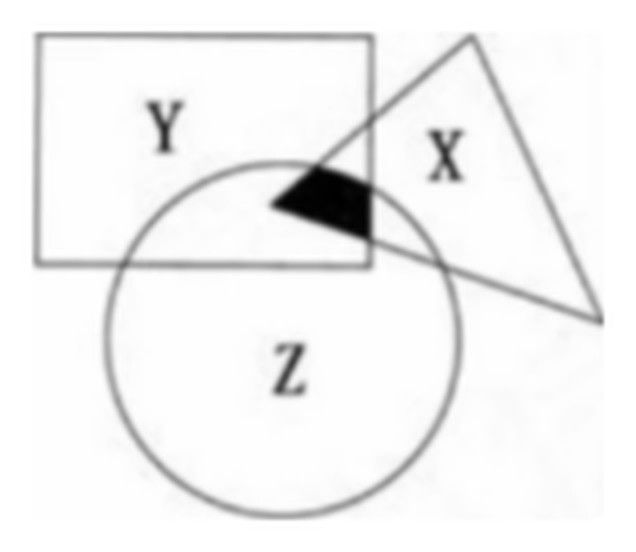
\includegraphics[width=0.20\textwidth]{figures/venn_XYZ_overlap.png}
\end{center}

\ifanswer
\solbegin
\step{设阴影部分的面积是 $x$，则 $290=64+180+160-24-70-36+x$，}
\step{$290=274+x$，$x=16$，故阴影部分的面积是 $16$.}
\solend

\fi

\item 如果集合 $A=\{1,2,3,\cdots,8\}$ 的子集 $B$ 满足：若 $2k\in B$，$k\in\N^{*}$，则 $2k+1\in B$，则称 $B$ 为 $A$ 的“好子集”，$A$ 的“好子集”有 \blankline[2.4em] 个.

\ifanswer
\solbegin
\step{由“好子集”定义得 $2$，$3$ 同时出现，$4$，$5$ 同时出现，$6$，$7$ 同时出现，}
\step{①当集合 $B$ 为空集时，满足题意；}
% 注：原卷此行印作「非空真子集共有 $2^4-1=15$ 种」，与同行算式冲突（$2^4-1=15$ 是**非空子集**数，
%     非空真子集应为 $2^4-2=14$），且与本段①（$B=\varnothing$）合起来恰构成「不含偶数的全体子集」，
%     故按文意订正为「非空子集」（段末总数 $1+15+24+12+2=54$ 不变）。
\step{②当集合 $B$ 中不存在偶数时，$\{1,3,5,7\}$ 的非空子集共有 $2^4-1=15$ 种；}
\step{③当集合 $B$ 中存在 $1$ 个偶数时，三个偶数中选择 $1$ 个，有 $C_3^1=3$ 种，}
\step{剩下 $3$ 个奇数不选，选 $1$ 个、$2$ 个、$3$ 个共有 $2^3=8$ 种，故共有 $24$ 种；}
\step{④当集合 $B$ 中存在 $2$ 个偶数时，三个偶数中选择 $2$ 个，有 $C_3^2=3$ 种，}
\step{剩下 $2$ 个奇数不选，选 $1$ 个、$2$ 个共有 $2^2=4$ 种，故共有 $12$ 种；}
\step{⑤当集合 $B$ 中存在 $3$ 个偶数时，三个偶数中选择 $3$ 个，有 $C_3^3=1$ 种，}
\step{剩下 $1$ 个奇数不选，选 $1$ 个共有 $2^1=2$ 种，故共有 $2$ 种；}
\step{所以 $A$ 的“好子集”共有 $1+15+24+12+2=54$ 种.}
\solend

\fi

\item 已知 $A=\{x\mid x=a^2-b^2,\ a\in\Z,b\in\Z,x\in\N^{*},x\leqslant 40\}$，则集合 $A$ 中共有 \blankline[2.4em] 个元素.

\ifanswer
\solbegin
\step{因为 $(k+1)^2-k^2=2k+1$，所以所有正奇数都属于集合 $A$，}
\step{又 $(2k+2)^2-(2k)^2=8k+4=4(2k+1)$，$(2k+1)^2-(2k-1)^2=8k=4\times 2k$，}
\step{因此所有 $4$ 的整数倍的正整数也属于 $A$，}
\step{若 $x=4k+2$，$k\in\N$，则 $a^2-b^2=(a+b)(a-b)=4k+2=2(2k+1)$，}
\step{则 $a+b$ 和 $a-b$ 中一定是一个取奇数，一个取偶数，}
\step{但是 $a,b\in\Z$ 时，$a+b$ 与 $a-b$ 同奇偶，所以此时无解，}
\step{即所有被 $4$ 除余 $2$ 的正整数都不属于 $A$，}
\step{所以每 $4$ 个数中，有 $3$ 个数属于集合 $A$，则集合 $A$ 中共含 $30$ 个元素.}
\solend

\fi

\item 十个元素组成的集合 $M=\{19,93,-1,0,25,-78,-94,1,17,-2\}$，$M$ 的所有非空子集记为 $M_i$（$i=1,2,\cdots,1023$），每一非空子集中所有元素的乘积记为 $m_i$（$i=1,2,\cdots,1023$），则 $m_1+m_2+\cdots+m_{1023}=$ \blankline[3em].

\ifanswer
\solbegin
\step{因为 $M$ 的所有非空子集为 $M_i$（$i=1,2,\cdots,1023$），这 $1023$ 个子集分成以下几种情况：}
\step{①含 $0$ 的子集有 $512$ 个，这些子集均满足 $m_i=0$；}
\step{②不含 $0$，含 $-1$ 且还含有其它元素的子集有 $255$ 个，}
\step{③不含 $0$，不含 $-1$ 但含有其它元素的子集有 $255$ 个，}
\step{④只含 $-1$ 的子集一个 $\{-1\}$，满足 $m_i=-1$；}
\step{其中②③中的集合是一一对应的，且满足 $m_i$ 对应成相反数，}
\step{故 $m_1+m_2+m_3+\cdots+m_{1023}=512\times 0+255\times 0-1=-1$.}
\solend

\fi

\item 已知 $M=\{(x,y)\mid |xy|=a\}$，$N=\{(x,y)\mid |xy|+1=|x|+|y|\}$，若集合 $M\cap N$ 中的点恰是正八边形的 $8$ 个顶点，则 $a=$ \blankline[2.4em].

\begin{center}
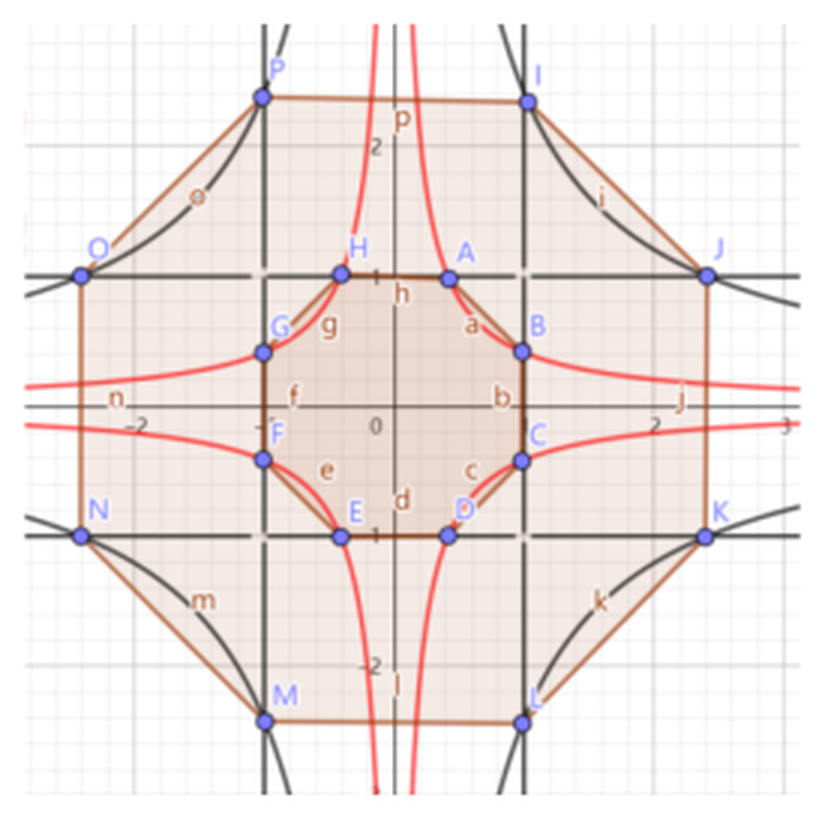
\includegraphics[width=0.44\textwidth]{figures/hyperbola_octagon.png}
\end{center}

\ifanswer
\solbegin
\step{$|xy|=a$ 和 $|xy|+1=|x|+|y|$ 的图像关于坐标轴均对称，只需考虑第一象限即可，}
\step{当 $x>0$，$y>0$ 时，$|xy|+1=|x|+|y|$ 即 $xy+1=x+y$，}
\step{即 $(x-1)(y-1)=0$，}
\step{即 $x=1$ 或 $y=1$，由对称性，作出完整的图像，}
\step{对于 $|xy|=a$，为四段双曲线，}
\step{考虑点 $A(I)(a,1)$，$B(J)(1,a)$，$C(K)(1,-a)$，}
\step{由 $AB=AC$ 得 $\sqrt{(a-1)^2+(1-a)^2}=2a$，解得 $a=\sqrt{2}\pm 1$.}
\solend

\fi

\item 集合 $A$ 是 $\{1,2,3,\cdots,100\}$ 的子集，若 $x\in A$，则 $2x\notin A$，$A$ 中的元素最多有 \blankline[2.4em] 个.

\ifanswer
\solbegin
\step{显然 $51$ 到 $100$ 共 $50$ 个可以，那么从 $1$ 到 $25$ 再 $2$ 倍不会超过 $50$，}
\step{$1$ 到 $25$ 中所有奇数都可以放到子集中，共有 $13$ 个，}
\step{再看偶数，$24=2\times 12$，$22=2\times 11$，$20=2\times 10$，$18=2\times 9$，$16=2\times 8$，}
% 注：末行照原卷抄录。原卷上一行列出 5 个偶数（24、22、20、18、16）而结论写「共有 $50+13+4=67$」，
%     此处的 $4$ 应作「另加 4 个元素」解（穷举验证集合 $A$ 的最大元素数确为 67），非笔误，故不改。
\step{及最后的 $4$，所以，共有 $50+13+4=67$.}
\solend

\fi

\end{enumerate}

\bigsec{二、选择题}

\begin{enumerate}
\setcounter{enumi}{13}

\item 下列各组集合中相等的是（\quad）.

①$P=\{x\mid x=2n,n\in\Z\}$，$Q=\{x\mid x=2(n-1),n\in\Z\}$；

②$P=\{x\mid x^2-1=0\}$，$Q=\left\{x\left|x=\dfrac{1+(-1)^n}{2},n\in\Z\right.\right\}$；

③$P=\{x\mid x=2m+1,m\in\Z\}$，$Q=\{x\mid x=4m\pm 1,m\in\Z\}$；

④$P=\{y\mid y=x^2+1\}$，$Q=\{x\mid y=x^2+1\}$.

\keepwithprev
A. ①②③④\qquad B. ①③\qquad C. ①②④\qquad D. ②④

\ans{B}

\item 如果一个命题的逆命题是真命题，那么这个命题的否命题是（\quad）

\keepwithprev
A. 真命题\qquad B. 假命题

C. 不一定是真命题\qquad D. 不一定是假命题

\ans{A}

\ifanswer
\solbegin
\step{一个命题的逆命题与这个命题的否命题是逆否命题，}
\step{它们的真假性相同，所以逆命题是真命题时，它们的否命题也是真命题. 故选 A.}
\solend

\fi

\item 设 $U$ 表示全集，下列命题中假命题有（\quad）

①若 $A\cap B=U$，则 $A=B=U$；②若 $A\cup B=\varnothing$，则 $A=B=\varnothing$；

③若 $A\cap B=\varnothing$，则 $\overline{A}\cup\overline{B}=U$；④若 $A\cup B=U$，则 $\overline{A}\cap\overline{B}=\varnothing$；

⑤若 $A\subseteq B$，则 $\overline{A}\supseteq\overline{B}$；⑥$\varnothing\in\{\varnothing\}$；⑦$\varnothing\subseteq\{\varnothing\}$.

\keepwithprev
A. $0$\qquad B. $1$\qquad C. $2$\qquad D. $3$

\ans{A}

\ifanswer
\solbegin
\step{全部正确，故选 A.}
\solend

\fi

\end{enumerate}

\bigsec{三、解答题}

\begin{enumerate}
\setcounter{enumi}{16}

\item 已知集合 $A=\{x\mid x^2-3x+2=0\}$，$B=\{x\mid x^2-bx+b-1=0\}$，$C=\{x\mid x^2-cx+2=0\}$.

\begin{enumerate}[label=(\arabic*)]
\item 若 $A\cup B=A$，求实数 $b$ 的值；
\item 若 $A\cap C=C$，求实数 $c$ 的取值范围.
\end{enumerate}

\ifanswer
\solbegin
\stepm{(1)}{$A=\{1,2\}$，$B=\{x\mid(x-1)(x-b+1)=0\}$，}
\step{由 $A\cup B=A$ 得 $b-1=1$ 或 $b-1=2$，所以 $b=2$ 或 $b=3$.}
\stepm{(2)}{由 $A\cap C=C$ 得 $C\subseteq A$，则 $C=\varnothing$ 或 $C=\{1\}$ 或 $C=\{2\}$ 或 $C=\{1,2\}$，}
\step{若 $C=\varnothing$，则 $\Delta=c^2-8<0$，解得 $-2\sqrt{2}<c<2\sqrt{2}$；}
\step{若 $C=\{1\}$，则 $\begin{cases}1+1=c\\ 1\times 1=2\end{cases}$，不可能；}
\step{若 $C=\{2\}$，则 $\begin{cases}2+2=c\\ 2\times 2=2\end{cases}$，不可能；}
\step{若 $C=\{1,2\}$，则 $\begin{cases}1+2=c\\ 1\times 2=2\end{cases}$，符合题意，$c=3$.}
\step{综上所述，$-2\sqrt{2}<c<2\sqrt{2}$ 或 $c=3$.}
\solend

\fi

\ansspace[6]

\item 已知全集 $U=\R$，$A=\{x\mid x^2+px+12=0\}$，$B=\{x\mid x^2-5x+q=0\}$，$\overline{A}\cap B=\{2\}$，求 $p+q$ 的值.

\ifanswer
\solbegin
\step{因为 $\overline{A}\cap B=\{2\}$，所以 $2\in B$，$2\notin A$，}
\step{所以 $2^2-5\times 2+q=0$，解得 $q=6$，$B=\{2,3\}$，}
\step{因为 $\overline{A}\cap B=\{2\}$，$B=\{2,3\}$，所以 $3\in A$，}
\step{所以 $3^2+p\times 3+12=0$，所以 $p=-7$，所以 $p+q=-1$.}
\solend

\fi

\ansspace[5]

\item 求证：方程 $x^2-abx+a+b=0$，$x^2-(a+b)x+ab=0$，其中 $a>2$，$b>2$ 没有公共根.

\ifanswer
\solbegin
\step{假设这两个方程有公共根 $\alpha$，则 $\alpha^2-ab\alpha+(a+b)=0$，$\alpha^2-(a+b)\alpha+ab=0$，}
\step{两式相减得 $(ab-a-b)(\alpha+1)=0$，}
\step{因为 $a>2$，$b>2$，所以 $a-1>1$，$b-1>1$，所以 $(a-1)(b-1)>1$，}
\step{所以 $ab-a-b>0$，所以 $\alpha+1=0$，所以 $\alpha=-1$，}
\step{代入第一个方程，得 $1+ab+a+b=0$，即 $(a+1)(b+1)=0$，}
\step{因为 $a>2$，$b>2$，所以该式不成立，所以这两个方程没有公共根.}
\solend

\fi

\ansspace[9]

% 压轴题：其后已无内容，故作答区全用可丢弃胶水（\ansspace*），并在题目前先量一下版面。
\ansneed{7cm}

\item 若集合 $A$ 具有以下性质：①$0\in A$，$1\in A$；②若 $x$、$y\in A$，则 $x-y\in A$，且 $x\neq 0$ 时，$\dfrac{1}{x}\in A$；则称集合 $A$ 是“好集”.

\begin{enumerate}[label=(\arabic*)]
\item 分别判断集合 $B=\{-1,0,1\}$，有理数集 $\Q$ 是否是“好集”，并说明理由；
\item 设集合 $A$ 是“好集”，求证：若 $x$、$y\in A$，则 $x+y\in A$；
\item 对任意的一个“好集” $A$，分别判断下面命题的真假，并说明理由.

命题 $p$：若 $x$、$y\in A$，则必有 $xy\in A$；

命题 $q$：若 $x$、$y\in A$，且 $x\neq 0$，则必有 $\dfrac{y}{x}\in A$.
\end{enumerate}

\ifanswer
\solbegin
\stepm{(1)}{集合 $B$ 不是“好集”. 理由是：假设集合 $B$ 是“好集”.}
\step{因为 $-1\in B$，$1\in B$，所以 $-1-1=-2\in B$. 这与 $-2\notin B$ 矛盾.}
\step{有理数集 $\Q$ 是“好集”. 因为 $0\in\Q$，$1\in\Q$，}
\step{对任意的 $x$、$y\in\Q$，有 $x-y\in\Q$，且 $x\neq 0$ 时，$\dfrac{1}{x}\in\Q$，}
\step{所以有理数集 $\Q$ 是“好集”.}
\stepm{(2)}{因为集合 $A$ 是“好集”，所以 $0\in A$.}
\step{若 $x$、$y\in A$，则 $0-y\in A$，即 $-y\in A$，所以 $x-(-y)\in A$，即 $x+y\in A$.}
\stepm{(3)}{命题 $p$、$q$ 均为真命题. 理由如下：}
\step{对任意一个“好集” $A$，任取 $x$、$y\in A$，}
\step{若 $x$、$y$ 中有 $0$ 或 $1$ 时，显然 $xy\in A$.}
\step{下设 $x$、$y$ 均不为 $0$，$1$. 由定义得 $x-1$，$\dfrac{1}{x-1}$，$\dfrac{1}{x}\in A$，}
\step{所以 $\dfrac{1}{x-1}-\dfrac{1}{x}\in A$，即 $\dfrac{1}{x(x-1)}\in A$，所以 $x(x-1)\in A$.}
\step{由（2）得 $x(x-1)+x\in A$，即 $x^2\in A$. 同理可得 $y^2\in A$.}
\step{若 $x+y=0$ 或 $x+y=1$，则 $x^2+y^2\in A$.}
\step{若 $x+y\neq 0$ 且 $x+y\neq 1$，则 $(x+y)^2\in A$，}
\step{所以 $2xy=(x+y)^2-x^2-y^2\in A$，所以 $\dfrac{1}{2xy}\in A$，}
\step{由（2）得 $\dfrac{1}{xy}=\dfrac{1}{2xy}+\dfrac{1}{2xy}\in A$，所以 $xy\in A$.}
\step{综上，$xy\in A$，即命题 $p$ 为真命题.}
\step{若 $x$、$y\in A$，且 $x\neq 0$，则 $\dfrac{1}{x}\in A$，}
\step{所以 $\dfrac{y}{x}=y\cdot\dfrac{1}{x}\in A$，即命题 $q$ 为真命题.}
\solend

\fi

\ansspace*[11]

\end{enumerate}

\end{document}
"
% 紧凑版：xelatex "\def\iscompact{1}% 高一14_华师大二附中_集合与逻辑单元练习.tex
%   —— 高一上数学「2026-2027 年华师大二附中高一上 集合与逻辑单元练习」（试卷版/答案版）
% 试卷版：xelatex 高一14_华师大二附中_集合与逻辑单元练习.tex
% 答案版：xelatex "\def\isanswer{1}\input{高一14_华师大二附中_集合与逻辑单元练习.tex}"
% 紧凑版：xelatex "\def\iscompact{1}\input{高一14_华师大二附中_集合与逻辑单元练习.tex}"
%
% 原始材料是微信公众号图文（「魔都数学加油站」），正文为 6 张 PNG 页（1080×1527）。
% 原文本身就是一份**讲评版**——题目下方直接印出【答案】或【解析】，选择题更是把答案
% 直接印在括注里（第 14 题）。试题文字、答案与解析均照原卷录入，未改内容。卷面上的
% 粉色斜水印「魔都数学加油站」属水印，未录入。
%
% 与原卷的排版差异（均已在 README「说明」中交代）：
%   ① 原文自**第 3 题**起（第 1、2 题未在该文中发布），故本稿题号亦自 3 起；
%   ② 原卷未印分节标题，本稿按题型补出「一、填空题」「二、选择题」「三、解答题」三节；
%   ③ 原卷填空、选择题的答案直接印在题目下方（第 14 题印在括注里），本稿统一改为
%      试卷版隐去、答案版以【答案】或【解析】给出，使两版彻底分离；
%   ④ 原卷的 $\R$、$\Q$、$\Z$、$\N$、$\N^{*}$ 时作正体 $R$、$Q$、$Z$、$N$、$N^*$，
%      本稿按全稿惯例统一写作 $\R$、$\Q$、$\Z$、$\N$、$\N^{*}$；
%   ⑤ 原卷中文括注用**半角**括号（第 4 题「(填“真”或“假”)」、第 15 题「是(  )」、
%      第 16 题「有(    )」，均已放大核实），本稿按全稿惯例排全角；
%   ⑥ 第 3 题题干作「$a$ 为**指定**实数」、同题解析作「$a$ 为**给定**的实数」，二者同义，
%      本稿两处均照原卷抄录（未统一）。

% 原卷笔误一处（已逐处放大到能看清字形后核对，本稿按文意订正，并在 README 中写明原委）：
%   ① 第 9 题【解析】② 原卷印「$\{1,3,5,7\}$ 的非空**真**子集共有 $2^4-1=15$ 种」，
%      与同行算式冲突（$2^4-1=15$ 是**非空子集**数，非空真子集应为 $2^4-2=14$），
%      且与本段①（$B=\varnothing$）合起来恰构成「不含偶数的全体子集」，故订正为「非空子集」，
%      段末总数 $1+15+24+12+2=54$ 不变。
%
% 原卷存疑一处（无法确证原意，本稿照抄并加 % 注）：
%   ① 第 12 题【解析】末行「由 $AB=AC$ 得 $\sqrt{(a-1)^2+(1-a)^2}=2a$，解得 $a=\sqrt2\pm1$」——
%      按此式只能解出 $a=\sqrt2-1$（$a=\sqrt2+1$ 处左端 $2$、右端 $4.83$，等式不成立），
%      而其答案 $a=\sqrt2\pm1$ 经数值验证是正确的（两值互为倒数，均使 $M\cap N$ 的 8 个交点按
%      $45^\circ$ 均布）。疑为解析此式笔误，但无法确证原意，本稿照抄原卷、未改。
%      同行上一行的「考虑点 $A(I)(a,1)$，$B(J)(1,a)$，$C(K)(1,-a)$」（点标 I/J/K 与
%      figures/hyperbola_octagon.png 中的标注一一对应）与本行等号右端的 $2a$，均照原卷录入；
%      2026-09-15 回原图逐处放大复核时发现曾误作 $A(1,a)$、$B(a,1)$、$C(-1,a)$ 与「$=2$」，
%      已按原卷订正（见 README「高一14—高一18 专记」）。

\documentclass[a4paper,11pt]{article}
\usepackage{common}

\begin{document}

\examtitlest[3]{2026--2027 年华师大二附中高一上}{集合与逻辑单元练习}

\bigsec{一、填空题}

\begin{enumerate}
\setcounter{enumi}{2}

\item 已知 $a$ 为指定实数，$M=\{x\mid x^2-3x-a^2+2=0\}$ 的非空真子集个数是 \blankline[2.4em].

\ifanswer
\solbegin
\step{集合 $M=\{x\mid x^2-3x-a^2+2=0\}$，$a$ 为给定的实数，}
\step{关于方程 $x^2-3x-a^2+2=0$，因为 $\Delta=(-3)^2-4(2-a^2)=4a^2+1>0$，}
\step{所以方程有两个不同的实根，所以 $M$ 中有两个元素，}
\step{所以集合 $M$ 的非空真子集的个数为 $2^2-2=2$.}
\solend

\fi

\item 判断下列命题的真假：（填“真”或“假”）

（1）任何集合都不是空集的子集 \blankline[2.4em]；

（2）一个有理数与一个无理数的和与积都是无理数 \blankline[2.4em]；

（3）如果一个整数 $n$ 的平方是偶数，那么 $n$ 是偶数 \blankline[2.4em].

\ans{假，假，真}

\item 请写出“如果两个三角形全等，那么它们的面积相等”的逆否命题：\blankline[3em].

\ifanswer
\solbegin
\step{如果两个三角形的面积不相等，则这两个三角形不全等.}
\solend

\fi

\item 已知 $U=\{(x,y)\mid x,y\in\R\}$，$M=\left\{(x,y)\left|\dfrac{y-2}{x-1}=3\right.\right\}$，$N=\{(x,y)\mid y=3x-1\}$，$\overline{M}\cap N=$ \blankline[3em].

\ans{$\{(1,2)\}$}

\item 已知集合 $A=\{x\mid 5x-a\leqslant 0\}$，$B=\{x\mid 6x-b>0\}$，$a$、$b\in\N$，且 $A\cap B\cap\N=\{2,3,4\}$，则整数对 $(a,b)$ 的个数为 \blankline[2.4em].

\ifanswer
\solbegin
\step{$A=\left\{x\left|x\leqslant\dfrac{a}{5}\right.\right\}$，$B=\left\{x\left|x>\dfrac{b}{6}\right.\right\}$，因为 $A\cap B\cap\N=\{2,3,4\}$，}
\step{所以 $4\leqslant\dfrac{a}{5}<5$，$1\leqslant\dfrac{b}{6}<2$，解得 $20\leqslant a<25$，$6\leqslant b<12$，}
\step{又 $a$、$b\in\N$，所以 $a=20$，$21$，$22$，$23$，$24$，$b=6$，$7$，$8$，$9$，$10$，$11$，}
\step{则整数对 $(a,b)$ 的个数为 $30$.}
\solend

\fi

\item 如图所示，$X$、$Y$、$Z$ 分别是面积为 $64$、$180$、$160$ 的三张不同形状的纸片，它们部分重叠放在一起盖在桌面上，总共盖住的面积为 $290$，且 $X$ 与 $Y$、$Y$ 与 $Z$、$Z$ 与 $X$ 重叠部分面积分别为 $24$、$70$、$36$，问阴影部分的面积是 \blankline[2.4em].

\begin{center}
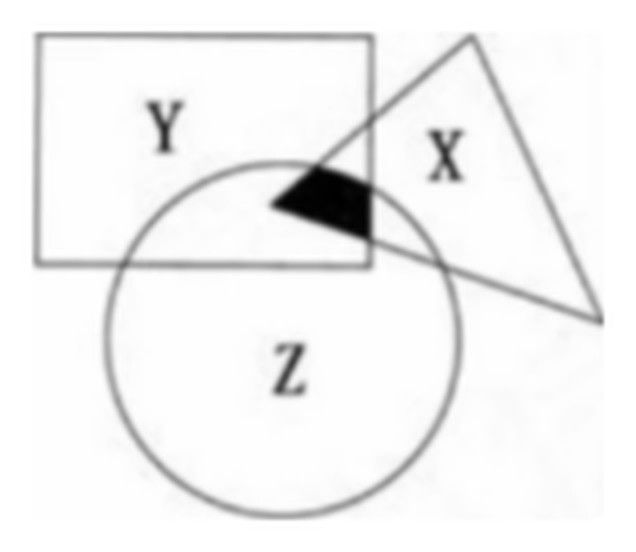
\includegraphics[width=0.20\textwidth]{figures/venn_XYZ_overlap.png}
\end{center}

\ifanswer
\solbegin
\step{设阴影部分的面积是 $x$，则 $290=64+180+160-24-70-36+x$，}
\step{$290=274+x$，$x=16$，故阴影部分的面积是 $16$.}
\solend

\fi

\item 如果集合 $A=\{1,2,3,\cdots,8\}$ 的子集 $B$ 满足：若 $2k\in B$，$k\in\N^{*}$，则 $2k+1\in B$，则称 $B$ 为 $A$ 的“好子集”，$A$ 的“好子集”有 \blankline[2.4em] 个.

\ifanswer
\solbegin
\step{由“好子集”定义得 $2$，$3$ 同时出现，$4$，$5$ 同时出现，$6$，$7$ 同时出现，}
\step{①当集合 $B$ 为空集时，满足题意；}
% 注：原卷此行印作「非空真子集共有 $2^4-1=15$ 种」，与同行算式冲突（$2^4-1=15$ 是**非空子集**数，
%     非空真子集应为 $2^4-2=14$），且与本段①（$B=\varnothing$）合起来恰构成「不含偶数的全体子集」，
%     故按文意订正为「非空子集」（段末总数 $1+15+24+12+2=54$ 不变）。
\step{②当集合 $B$ 中不存在偶数时，$\{1,3,5,7\}$ 的非空子集共有 $2^4-1=15$ 种；}
\step{③当集合 $B$ 中存在 $1$ 个偶数时，三个偶数中选择 $1$ 个，有 $C_3^1=3$ 种，}
\step{剩下 $3$ 个奇数不选，选 $1$ 个、$2$ 个、$3$ 个共有 $2^3=8$ 种，故共有 $24$ 种；}
\step{④当集合 $B$ 中存在 $2$ 个偶数时，三个偶数中选择 $2$ 个，有 $C_3^2=3$ 种，}
\step{剩下 $2$ 个奇数不选，选 $1$ 个、$2$ 个共有 $2^2=4$ 种，故共有 $12$ 种；}
\step{⑤当集合 $B$ 中存在 $3$ 个偶数时，三个偶数中选择 $3$ 个，有 $C_3^3=1$ 种，}
\step{剩下 $1$ 个奇数不选，选 $1$ 个共有 $2^1=2$ 种，故共有 $2$ 种；}
\step{所以 $A$ 的“好子集”共有 $1+15+24+12+2=54$ 种.}
\solend

\fi

\item 已知 $A=\{x\mid x=a^2-b^2,\ a\in\Z,b\in\Z,x\in\N^{*},x\leqslant 40\}$，则集合 $A$ 中共有 \blankline[2.4em] 个元素.

\ifanswer
\solbegin
\step{因为 $(k+1)^2-k^2=2k+1$，所以所有正奇数都属于集合 $A$，}
\step{又 $(2k+2)^2-(2k)^2=8k+4=4(2k+1)$，$(2k+1)^2-(2k-1)^2=8k=4\times 2k$，}
\step{因此所有 $4$ 的整数倍的正整数也属于 $A$，}
\step{若 $x=4k+2$，$k\in\N$，则 $a^2-b^2=(a+b)(a-b)=4k+2=2(2k+1)$，}
\step{则 $a+b$ 和 $a-b$ 中一定是一个取奇数，一个取偶数，}
\step{但是 $a,b\in\Z$ 时，$a+b$ 与 $a-b$ 同奇偶，所以此时无解，}
\step{即所有被 $4$ 除余 $2$ 的正整数都不属于 $A$，}
\step{所以每 $4$ 个数中，有 $3$ 个数属于集合 $A$，则集合 $A$ 中共含 $30$ 个元素.}
\solend

\fi

\item 十个元素组成的集合 $M=\{19,93,-1,0,25,-78,-94,1,17,-2\}$，$M$ 的所有非空子集记为 $M_i$（$i=1,2,\cdots,1023$），每一非空子集中所有元素的乘积记为 $m_i$（$i=1,2,\cdots,1023$），则 $m_1+m_2+\cdots+m_{1023}=$ \blankline[3em].

\ifanswer
\solbegin
\step{因为 $M$ 的所有非空子集为 $M_i$（$i=1,2,\cdots,1023$），这 $1023$ 个子集分成以下几种情况：}
\step{①含 $0$ 的子集有 $512$ 个，这些子集均满足 $m_i=0$；}
\step{②不含 $0$，含 $-1$ 且还含有其它元素的子集有 $255$ 个，}
\step{③不含 $0$，不含 $-1$ 但含有其它元素的子集有 $255$ 个，}
\step{④只含 $-1$ 的子集一个 $\{-1\}$，满足 $m_i=-1$；}
\step{其中②③中的集合是一一对应的，且满足 $m_i$ 对应成相反数，}
\step{故 $m_1+m_2+m_3+\cdots+m_{1023}=512\times 0+255\times 0-1=-1$.}
\solend

\fi

\item 已知 $M=\{(x,y)\mid |xy|=a\}$，$N=\{(x,y)\mid |xy|+1=|x|+|y|\}$，若集合 $M\cap N$ 中的点恰是正八边形的 $8$ 个顶点，则 $a=$ \blankline[2.4em].

\begin{center}
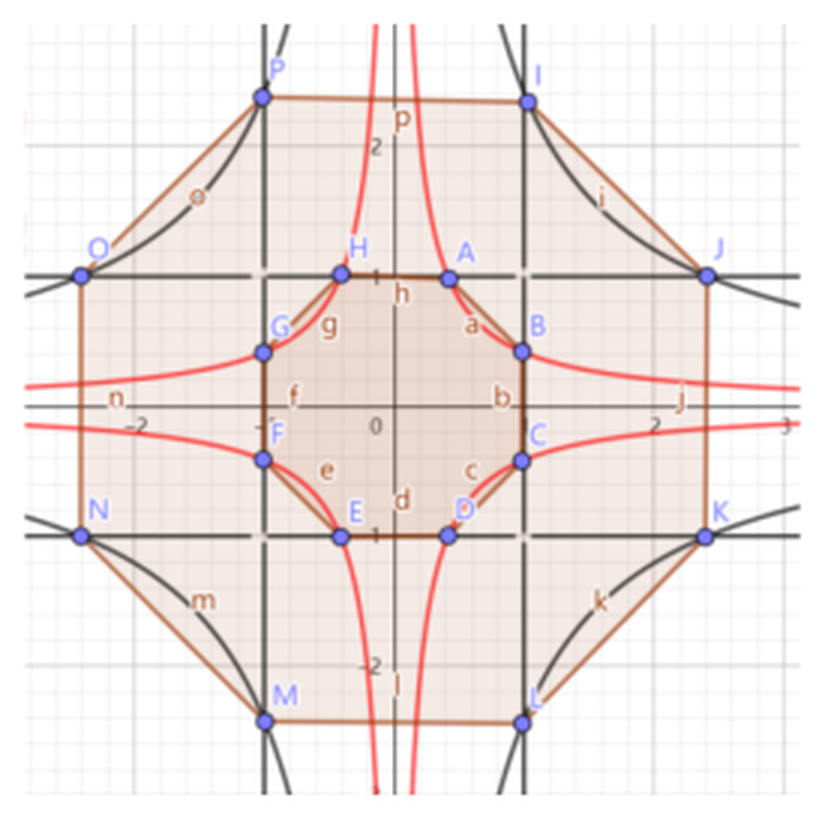
\includegraphics[width=0.44\textwidth]{figures/hyperbola_octagon.png}
\end{center}

\ifanswer
\solbegin
\step{$|xy|=a$ 和 $|xy|+1=|x|+|y|$ 的图像关于坐标轴均对称，只需考虑第一象限即可，}
\step{当 $x>0$，$y>0$ 时，$|xy|+1=|x|+|y|$ 即 $xy+1=x+y$，}
\step{即 $(x-1)(y-1)=0$，}
\step{即 $x=1$ 或 $y=1$，由对称性，作出完整的图像，}
\step{对于 $|xy|=a$，为四段双曲线，}
\step{考虑点 $A(I)(a,1)$，$B(J)(1,a)$，$C(K)(1,-a)$，}
\step{由 $AB=AC$ 得 $\sqrt{(a-1)^2+(1-a)^2}=2a$，解得 $a=\sqrt{2}\pm 1$.}
\solend

\fi

\item 集合 $A$ 是 $\{1,2,3,\cdots,100\}$ 的子集，若 $x\in A$，则 $2x\notin A$，$A$ 中的元素最多有 \blankline[2.4em] 个.

\ifanswer
\solbegin
\step{显然 $51$ 到 $100$ 共 $50$ 个可以，那么从 $1$ 到 $25$ 再 $2$ 倍不会超过 $50$，}
\step{$1$ 到 $25$ 中所有奇数都可以放到子集中，共有 $13$ 个，}
\step{再看偶数，$24=2\times 12$，$22=2\times 11$，$20=2\times 10$，$18=2\times 9$，$16=2\times 8$，}
% 注：末行照原卷抄录。原卷上一行列出 5 个偶数（24、22、20、18、16）而结论写「共有 $50+13+4=67$」，
%     此处的 $4$ 应作「另加 4 个元素」解（穷举验证集合 $A$ 的最大元素数确为 67），非笔误，故不改。
\step{及最后的 $4$，所以，共有 $50+13+4=67$.}
\solend

\fi

\end{enumerate}

\bigsec{二、选择题}

\begin{enumerate}
\setcounter{enumi}{13}

\item 下列各组集合中相等的是（\quad）.

①$P=\{x\mid x=2n,n\in\Z\}$，$Q=\{x\mid x=2(n-1),n\in\Z\}$；

②$P=\{x\mid x^2-1=0\}$，$Q=\left\{x\left|x=\dfrac{1+(-1)^n}{2},n\in\Z\right.\right\}$；

③$P=\{x\mid x=2m+1,m\in\Z\}$，$Q=\{x\mid x=4m\pm 1,m\in\Z\}$；

④$P=\{y\mid y=x^2+1\}$，$Q=\{x\mid y=x^2+1\}$.

\keepwithprev
A. ①②③④\qquad B. ①③\qquad C. ①②④\qquad D. ②④

\ans{B}

\item 如果一个命题的逆命题是真命题，那么这个命题的否命题是（\quad）

\keepwithprev
A. 真命题\qquad B. 假命题

C. 不一定是真命题\qquad D. 不一定是假命题

\ans{A}

\ifanswer
\solbegin
\step{一个命题的逆命题与这个命题的否命题是逆否命题，}
\step{它们的真假性相同，所以逆命题是真命题时，它们的否命题也是真命题. 故选 A.}
\solend

\fi

\item 设 $U$ 表示全集，下列命题中假命题有（\quad）

①若 $A\cap B=U$，则 $A=B=U$；②若 $A\cup B=\varnothing$，则 $A=B=\varnothing$；

③若 $A\cap B=\varnothing$，则 $\overline{A}\cup\overline{B}=U$；④若 $A\cup B=U$，则 $\overline{A}\cap\overline{B}=\varnothing$；

⑤若 $A\subseteq B$，则 $\overline{A}\supseteq\overline{B}$；⑥$\varnothing\in\{\varnothing\}$；⑦$\varnothing\subseteq\{\varnothing\}$.

\keepwithprev
A. $0$\qquad B. $1$\qquad C. $2$\qquad D. $3$

\ans{A}

\ifanswer
\solbegin
\step{全部正确，故选 A.}
\solend

\fi

\end{enumerate}

\bigsec{三、解答题}

\begin{enumerate}
\setcounter{enumi}{16}

\item 已知集合 $A=\{x\mid x^2-3x+2=0\}$，$B=\{x\mid x^2-bx+b-1=0\}$，$C=\{x\mid x^2-cx+2=0\}$.

\begin{enumerate}[label=(\arabic*)]
\item 若 $A\cup B=A$，求实数 $b$ 的值；
\item 若 $A\cap C=C$，求实数 $c$ 的取值范围.
\end{enumerate}

\ifanswer
\solbegin
\stepm{(1)}{$A=\{1,2\}$，$B=\{x\mid(x-1)(x-b+1)=0\}$，}
\step{由 $A\cup B=A$ 得 $b-1=1$ 或 $b-1=2$，所以 $b=2$ 或 $b=3$.}
\stepm{(2)}{由 $A\cap C=C$ 得 $C\subseteq A$，则 $C=\varnothing$ 或 $C=\{1\}$ 或 $C=\{2\}$ 或 $C=\{1,2\}$，}
\step{若 $C=\varnothing$，则 $\Delta=c^2-8<0$，解得 $-2\sqrt{2}<c<2\sqrt{2}$；}
\step{若 $C=\{1\}$，则 $\begin{cases}1+1=c\\ 1\times 1=2\end{cases}$，不可能；}
\step{若 $C=\{2\}$，则 $\begin{cases}2+2=c\\ 2\times 2=2\end{cases}$，不可能；}
\step{若 $C=\{1,2\}$，则 $\begin{cases}1+2=c\\ 1\times 2=2\end{cases}$，符合题意，$c=3$.}
\step{综上所述，$-2\sqrt{2}<c<2\sqrt{2}$ 或 $c=3$.}
\solend

\fi

\ansspace[6]

\item 已知全集 $U=\R$，$A=\{x\mid x^2+px+12=0\}$，$B=\{x\mid x^2-5x+q=0\}$，$\overline{A}\cap B=\{2\}$，求 $p+q$ 的值.

\ifanswer
\solbegin
\step{因为 $\overline{A}\cap B=\{2\}$，所以 $2\in B$，$2\notin A$，}
\step{所以 $2^2-5\times 2+q=0$，解得 $q=6$，$B=\{2,3\}$，}
\step{因为 $\overline{A}\cap B=\{2\}$，$B=\{2,3\}$，所以 $3\in A$，}
\step{所以 $3^2+p\times 3+12=0$，所以 $p=-7$，所以 $p+q=-1$.}
\solend

\fi

\ansspace[5]

\item 求证：方程 $x^2-abx+a+b=0$，$x^2-(a+b)x+ab=0$，其中 $a>2$，$b>2$ 没有公共根.

\ifanswer
\solbegin
\step{假设这两个方程有公共根 $\alpha$，则 $\alpha^2-ab\alpha+(a+b)=0$，$\alpha^2-(a+b)\alpha+ab=0$，}
\step{两式相减得 $(ab-a-b)(\alpha+1)=0$，}
\step{因为 $a>2$，$b>2$，所以 $a-1>1$，$b-1>1$，所以 $(a-1)(b-1)>1$，}
\step{所以 $ab-a-b>0$，所以 $\alpha+1=0$，所以 $\alpha=-1$，}
\step{代入第一个方程，得 $1+ab+a+b=0$，即 $(a+1)(b+1)=0$，}
\step{因为 $a>2$，$b>2$，所以该式不成立，所以这两个方程没有公共根.}
\solend

\fi

\ansspace[9]

% 压轴题：其后已无内容，故作答区全用可丢弃胶水（\ansspace*），并在题目前先量一下版面。
\ansneed{7cm}

\item 若集合 $A$ 具有以下性质：①$0\in A$，$1\in A$；②若 $x$、$y\in A$，则 $x-y\in A$，且 $x\neq 0$ 时，$\dfrac{1}{x}\in A$；则称集合 $A$ 是“好集”.

\begin{enumerate}[label=(\arabic*)]
\item 分别判断集合 $B=\{-1,0,1\}$，有理数集 $\Q$ 是否是“好集”，并说明理由；
\item 设集合 $A$ 是“好集”，求证：若 $x$、$y\in A$，则 $x+y\in A$；
\item 对任意的一个“好集” $A$，分别判断下面命题的真假，并说明理由.

命题 $p$：若 $x$、$y\in A$，则必有 $xy\in A$；

命题 $q$：若 $x$、$y\in A$，且 $x\neq 0$，则必有 $\dfrac{y}{x}\in A$.
\end{enumerate}

\ifanswer
\solbegin
\stepm{(1)}{集合 $B$ 不是“好集”. 理由是：假设集合 $B$ 是“好集”.}
\step{因为 $-1\in B$，$1\in B$，所以 $-1-1=-2\in B$. 这与 $-2\notin B$ 矛盾.}
\step{有理数集 $\Q$ 是“好集”. 因为 $0\in\Q$，$1\in\Q$，}
\step{对任意的 $x$、$y\in\Q$，有 $x-y\in\Q$，且 $x\neq 0$ 时，$\dfrac{1}{x}\in\Q$，}
\step{所以有理数集 $\Q$ 是“好集”.}
\stepm{(2)}{因为集合 $A$ 是“好集”，所以 $0\in A$.}
\step{若 $x$、$y\in A$，则 $0-y\in A$，即 $-y\in A$，所以 $x-(-y)\in A$，即 $x+y\in A$.}
\stepm{(3)}{命题 $p$、$q$ 均为真命题. 理由如下：}
\step{对任意一个“好集” $A$，任取 $x$、$y\in A$，}
\step{若 $x$、$y$ 中有 $0$ 或 $1$ 时，显然 $xy\in A$.}
\step{下设 $x$、$y$ 均不为 $0$，$1$. 由定义得 $x-1$，$\dfrac{1}{x-1}$，$\dfrac{1}{x}\in A$，}
\step{所以 $\dfrac{1}{x-1}-\dfrac{1}{x}\in A$，即 $\dfrac{1}{x(x-1)}\in A$，所以 $x(x-1)\in A$.}
\step{由（2）得 $x(x-1)+x\in A$，即 $x^2\in A$. 同理可得 $y^2\in A$.}
\step{若 $x+y=0$ 或 $x+y=1$，则 $x^2+y^2\in A$.}
\step{若 $x+y\neq 0$ 且 $x+y\neq 1$，则 $(x+y)^2\in A$，}
\step{所以 $2xy=(x+y)^2-x^2-y^2\in A$，所以 $\dfrac{1}{2xy}\in A$，}
\step{由（2）得 $\dfrac{1}{xy}=\dfrac{1}{2xy}+\dfrac{1}{2xy}\in A$，所以 $xy\in A$.}
\step{综上，$xy\in A$，即命题 $p$ 为真命题.}
\step{若 $x$、$y\in A$，且 $x\neq 0$，则 $\dfrac{1}{x}\in A$，}
\step{所以 $\dfrac{y}{x}=y\cdot\dfrac{1}{x}\in A$，即命题 $q$ 为真命题.}
\solend

\fi

\ansspace*[11]

\end{enumerate}

\end{document}
"
%
% 原始材料是微信公众号图文（「魔都数学加油站」），正文为 6 张 PNG 页（1080×1527）。
% 原文本身就是一份**讲评版**——题目下方直接印出【答案】或【解析】，选择题更是把答案
% 直接印在括注里（第 14 题）。试题文字、答案与解析均照原卷录入，未改内容。卷面上的
% 粉色斜水印「魔都数学加油站」属水印，未录入。
%
% 与原卷的排版差异（均已在 README「说明」中交代）：
%   ① 原文自**第 3 题**起（第 1、2 题未在该文中发布），故本稿题号亦自 3 起；
%   ② 原卷未印分节标题，本稿按题型补出「一、填空题」「二、选择题」「三、解答题」三节；
%   ③ 原卷填空、选择题的答案直接印在题目下方（第 14 题印在括注里），本稿统一改为
%      试卷版隐去、答案版以【答案】或【解析】给出，使两版彻底分离；
%   ④ 原卷的 $\R$、$\Q$、$\Z$、$\N$、$\N^{*}$ 时作正体 $R$、$Q$、$Z$、$N$、$N^*$，
%      本稿按全稿惯例统一写作 $\R$、$\Q$、$\Z$、$\N$、$\N^{*}$；
%   ⑤ 原卷中文括注用**半角**括号（第 4 题「(填“真”或“假”)」、第 15 题「是(  )」、
%      第 16 题「有(    )」，均已放大核实），本稿按全稿惯例排全角；
%   ⑥ 第 3 题题干作「$a$ 为**指定**实数」、同题解析作「$a$ 为**给定**的实数」，二者同义，
%      本稿两处均照原卷抄录（未统一）。

% 原卷笔误一处（已逐处放大到能看清字形后核对，本稿按文意订正，并在 README 中写明原委）：
%   ① 第 9 题【解析】② 原卷印「$\{1,3,5,7\}$ 的非空**真**子集共有 $2^4-1=15$ 种」，
%      与同行算式冲突（$2^4-1=15$ 是**非空子集**数，非空真子集应为 $2^4-2=14$），
%      且与本段①（$B=\varnothing$）合起来恰构成「不含偶数的全体子集」，故订正为「非空子集」，
%      段末总数 $1+15+24+12+2=54$ 不变。
%
% 原卷存疑一处（无法确证原意，本稿照抄并加 % 注）：
%   ① 第 12 题【解析】末行「由 $AB=AC$ 得 $\sqrt{(a-1)^2+(1-a)^2}=2a$，解得 $a=\sqrt2\pm1$」——
%      按此式只能解出 $a=\sqrt2-1$（$a=\sqrt2+1$ 处左端 $2$、右端 $4.83$，等式不成立），
%      而其答案 $a=\sqrt2\pm1$ 经数值验证是正确的（两值互为倒数，均使 $M\cap N$ 的 8 个交点按
%      $45^\circ$ 均布）。疑为解析此式笔误，但无法确证原意，本稿照抄原卷、未改。
%      同行上一行的「考虑点 $A(I)(a,1)$，$B(J)(1,a)$，$C(K)(1,-a)$」（点标 I/J/K 与
%      figures/hyperbola_octagon.png 中的标注一一对应）与本行等号右端的 $2a$，均照原卷录入；
%      2026-09-15 回原图逐处放大复核时发现曾误作 $A(1,a)$、$B(a,1)$、$C(-1,a)$ 与「$=2$」，
%      已按原卷订正（见 README「高一14—高一18 专记」）。

\documentclass[a4paper,11pt]{article}
\usepackage{common}

\begin{document}

\examtitlest[3]{2026--2027 年华师大二附中高一上}{集合与逻辑单元练习}

\bigsec{一、填空题}

\begin{enumerate}
\setcounter{enumi}{2}

\item 已知 $a$ 为指定实数，$M=\{x\mid x^2-3x-a^2+2=0\}$ 的非空真子集个数是 \blankline[2.4em].

\ifanswer
\solbegin
\step{集合 $M=\{x\mid x^2-3x-a^2+2=0\}$，$a$ 为给定的实数，}
\step{关于方程 $x^2-3x-a^2+2=0$，因为 $\Delta=(-3)^2-4(2-a^2)=4a^2+1>0$，}
\step{所以方程有两个不同的实根，所以 $M$ 中有两个元素，}
\step{所以集合 $M$ 的非空真子集的个数为 $2^2-2=2$.}
\solend

\fi

\item 判断下列命题的真假：（填“真”或“假”）

（1）任何集合都不是空集的子集 \blankline[2.4em]；

（2）一个有理数与一个无理数的和与积都是无理数 \blankline[2.4em]；

（3）如果一个整数 $n$ 的平方是偶数，那么 $n$ 是偶数 \blankline[2.4em].

\ans{假，假，真}

\item 请写出“如果两个三角形全等，那么它们的面积相等”的逆否命题：\blankline[3em].

\ifanswer
\solbegin
\step{如果两个三角形的面积不相等，则这两个三角形不全等.}
\solend

\fi

\item 已知 $U=\{(x,y)\mid x,y\in\R\}$，$M=\left\{(x,y)\left|\dfrac{y-2}{x-1}=3\right.\right\}$，$N=\{(x,y)\mid y=3x-1\}$，$\overline{M}\cap N=$ \blankline[3em].

\ans{$\{(1,2)\}$}

\item 已知集合 $A=\{x\mid 5x-a\leqslant 0\}$，$B=\{x\mid 6x-b>0\}$，$a$、$b\in\N$，且 $A\cap B\cap\N=\{2,3,4\}$，则整数对 $(a,b)$ 的个数为 \blankline[2.4em].

\ifanswer
\solbegin
\step{$A=\left\{x\left|x\leqslant\dfrac{a}{5}\right.\right\}$，$B=\left\{x\left|x>\dfrac{b}{6}\right.\right\}$，因为 $A\cap B\cap\N=\{2,3,4\}$，}
\step{所以 $4\leqslant\dfrac{a}{5}<5$，$1\leqslant\dfrac{b}{6}<2$，解得 $20\leqslant a<25$，$6\leqslant b<12$，}
\step{又 $a$、$b\in\N$，所以 $a=20$，$21$，$22$，$23$，$24$，$b=6$，$7$，$8$，$9$，$10$，$11$，}
\step{则整数对 $(a,b)$ 的个数为 $30$.}
\solend

\fi

\item 如图所示，$X$、$Y$、$Z$ 分别是面积为 $64$、$180$、$160$ 的三张不同形状的纸片，它们部分重叠放在一起盖在桌面上，总共盖住的面积为 $290$，且 $X$ 与 $Y$、$Y$ 与 $Z$、$Z$ 与 $X$ 重叠部分面积分别为 $24$、$70$、$36$，问阴影部分的面积是 \blankline[2.4em].

\begin{center}
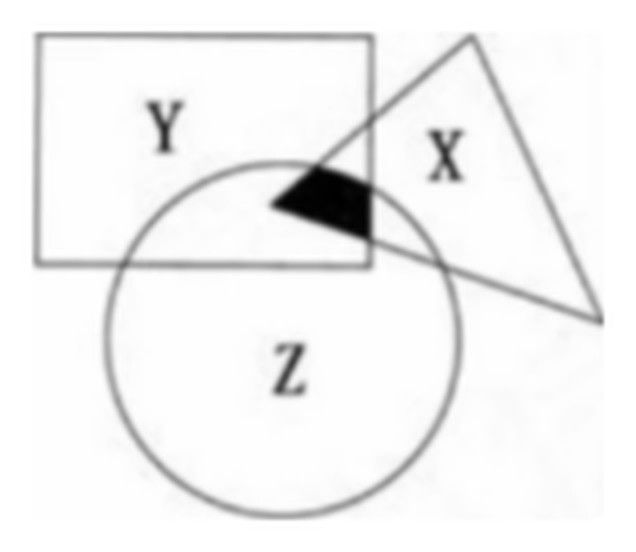
\includegraphics[width=0.20\textwidth]{figures/venn_XYZ_overlap.png}
\end{center}

\ifanswer
\solbegin
\step{设阴影部分的面积是 $x$，则 $290=64+180+160-24-70-36+x$，}
\step{$290=274+x$，$x=16$，故阴影部分的面积是 $16$.}
\solend

\fi

\item 如果集合 $A=\{1,2,3,\cdots,8\}$ 的子集 $B$ 满足：若 $2k\in B$，$k\in\N^{*}$，则 $2k+1\in B$，则称 $B$ 为 $A$ 的“好子集”，$A$ 的“好子集”有 \blankline[2.4em] 个.

\ifanswer
\solbegin
\step{由“好子集”定义得 $2$，$3$ 同时出现，$4$，$5$ 同时出现，$6$，$7$ 同时出现，}
\step{①当集合 $B$ 为空集时，满足题意；}
% 注：原卷此行印作「非空真子集共有 $2^4-1=15$ 种」，与同行算式冲突（$2^4-1=15$ 是**非空子集**数，
%     非空真子集应为 $2^4-2=14$），且与本段①（$B=\varnothing$）合起来恰构成「不含偶数的全体子集」，
%     故按文意订正为「非空子集」（段末总数 $1+15+24+12+2=54$ 不变）。
\step{②当集合 $B$ 中不存在偶数时，$\{1,3,5,7\}$ 的非空子集共有 $2^4-1=15$ 种；}
\step{③当集合 $B$ 中存在 $1$ 个偶数时，三个偶数中选择 $1$ 个，有 $C_3^1=3$ 种，}
\step{剩下 $3$ 个奇数不选，选 $1$ 个、$2$ 个、$3$ 个共有 $2^3=8$ 种，故共有 $24$ 种；}
\step{④当集合 $B$ 中存在 $2$ 个偶数时，三个偶数中选择 $2$ 个，有 $C_3^2=3$ 种，}
\step{剩下 $2$ 个奇数不选，选 $1$ 个、$2$ 个共有 $2^2=4$ 种，故共有 $12$ 种；}
\step{⑤当集合 $B$ 中存在 $3$ 个偶数时，三个偶数中选择 $3$ 个，有 $C_3^3=1$ 种，}
\step{剩下 $1$ 个奇数不选，选 $1$ 个共有 $2^1=2$ 种，故共有 $2$ 种；}
\step{所以 $A$ 的“好子集”共有 $1+15+24+12+2=54$ 种.}
\solend

\fi

\item 已知 $A=\{x\mid x=a^2-b^2,\ a\in\Z,b\in\Z,x\in\N^{*},x\leqslant 40\}$，则集合 $A$ 中共有 \blankline[2.4em] 个元素.

\ifanswer
\solbegin
\step{因为 $(k+1)^2-k^2=2k+1$，所以所有正奇数都属于集合 $A$，}
\step{又 $(2k+2)^2-(2k)^2=8k+4=4(2k+1)$，$(2k+1)^2-(2k-1)^2=8k=4\times 2k$，}
\step{因此所有 $4$ 的整数倍的正整数也属于 $A$，}
\step{若 $x=4k+2$，$k\in\N$，则 $a^2-b^2=(a+b)(a-b)=4k+2=2(2k+1)$，}
\step{则 $a+b$ 和 $a-b$ 中一定是一个取奇数，一个取偶数，}
\step{但是 $a,b\in\Z$ 时，$a+b$ 与 $a-b$ 同奇偶，所以此时无解，}
\step{即所有被 $4$ 除余 $2$ 的正整数都不属于 $A$，}
\step{所以每 $4$ 个数中，有 $3$ 个数属于集合 $A$，则集合 $A$ 中共含 $30$ 个元素.}
\solend

\fi

\item 十个元素组成的集合 $M=\{19,93,-1,0,25,-78,-94,1,17,-2\}$，$M$ 的所有非空子集记为 $M_i$（$i=1,2,\cdots,1023$），每一非空子集中所有元素的乘积记为 $m_i$（$i=1,2,\cdots,1023$），则 $m_1+m_2+\cdots+m_{1023}=$ \blankline[3em].

\ifanswer
\solbegin
\step{因为 $M$ 的所有非空子集为 $M_i$（$i=1,2,\cdots,1023$），这 $1023$ 个子集分成以下几种情况：}
\step{①含 $0$ 的子集有 $512$ 个，这些子集均满足 $m_i=0$；}
\step{②不含 $0$，含 $-1$ 且还含有其它元素的子集有 $255$ 个，}
\step{③不含 $0$，不含 $-1$ 但含有其它元素的子集有 $255$ 个，}
\step{④只含 $-1$ 的子集一个 $\{-1\}$，满足 $m_i=-1$；}
\step{其中②③中的集合是一一对应的，且满足 $m_i$ 对应成相反数，}
\step{故 $m_1+m_2+m_3+\cdots+m_{1023}=512\times 0+255\times 0-1=-1$.}
\solend

\fi

\item 已知 $M=\{(x,y)\mid |xy|=a\}$，$N=\{(x,y)\mid |xy|+1=|x|+|y|\}$，若集合 $M\cap N$ 中的点恰是正八边形的 $8$ 个顶点，则 $a=$ \blankline[2.4em].

\begin{center}
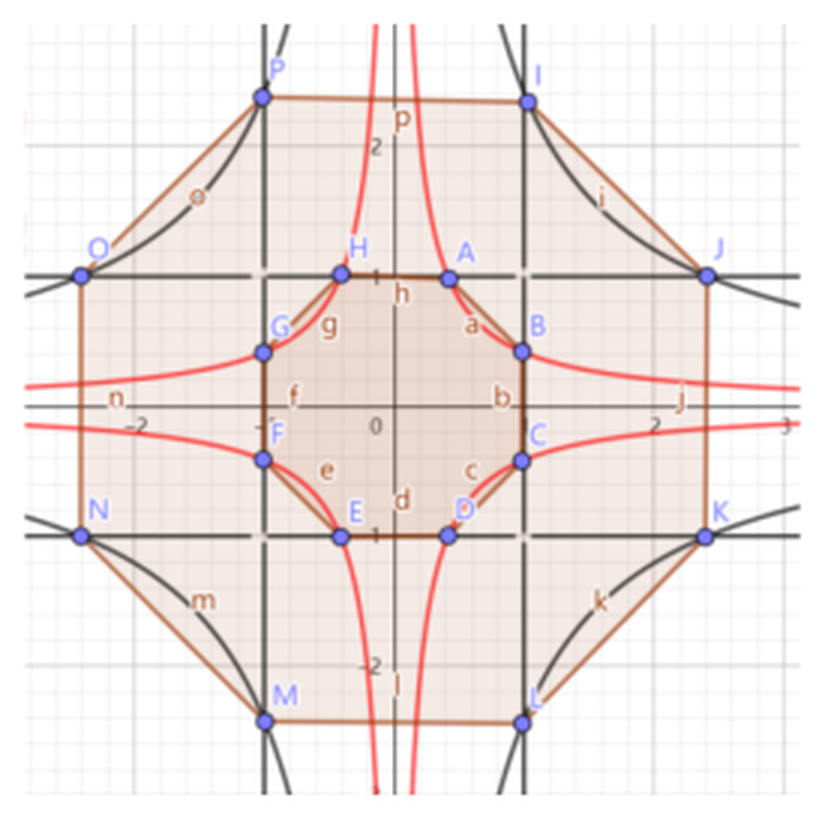
\includegraphics[width=0.44\textwidth]{figures/hyperbola_octagon.png}
\end{center}

\ifanswer
\solbegin
\step{$|xy|=a$ 和 $|xy|+1=|x|+|y|$ 的图像关于坐标轴均对称，只需考虑第一象限即可，}
\step{当 $x>0$，$y>0$ 时，$|xy|+1=|x|+|y|$ 即 $xy+1=x+y$，}
\step{即 $(x-1)(y-1)=0$，}
\step{即 $x=1$ 或 $y=1$，由对称性，作出完整的图像，}
\step{对于 $|xy|=a$，为四段双曲线，}
\step{考虑点 $A(I)(a,1)$，$B(J)(1,a)$，$C(K)(1,-a)$，}
\step{由 $AB=AC$ 得 $\sqrt{(a-1)^2+(1-a)^2}=2a$，解得 $a=\sqrt{2}\pm 1$.}
\solend

\fi

\item 集合 $A$ 是 $\{1,2,3,\cdots,100\}$ 的子集，若 $x\in A$，则 $2x\notin A$，$A$ 中的元素最多有 \blankline[2.4em] 个.

\ifanswer
\solbegin
\step{显然 $51$ 到 $100$ 共 $50$ 个可以，那么从 $1$ 到 $25$ 再 $2$ 倍不会超过 $50$，}
\step{$1$ 到 $25$ 中所有奇数都可以放到子集中，共有 $13$ 个，}
\step{再看偶数，$24=2\times 12$，$22=2\times 11$，$20=2\times 10$，$18=2\times 9$，$16=2\times 8$，}
% 注：末行照原卷抄录。原卷上一行列出 5 个偶数（24、22、20、18、16）而结论写「共有 $50+13+4=67$」，
%     此处的 $4$ 应作「另加 4 个元素」解（穷举验证集合 $A$ 的最大元素数确为 67），非笔误，故不改。
\step{及最后的 $4$，所以，共有 $50+13+4=67$.}
\solend

\fi

\end{enumerate}

\bigsec{二、选择题}

\begin{enumerate}
\setcounter{enumi}{13}

\item 下列各组集合中相等的是（\quad）.

①$P=\{x\mid x=2n,n\in\Z\}$，$Q=\{x\mid x=2(n-1),n\in\Z\}$；

②$P=\{x\mid x^2-1=0\}$，$Q=\left\{x\left|x=\dfrac{1+(-1)^n}{2},n\in\Z\right.\right\}$；

③$P=\{x\mid x=2m+1,m\in\Z\}$，$Q=\{x\mid x=4m\pm 1,m\in\Z\}$；

④$P=\{y\mid y=x^2+1\}$，$Q=\{x\mid y=x^2+1\}$.

\keepwithprev
A. ①②③④\qquad B. ①③\qquad C. ①②④\qquad D. ②④

\ans{B}

\item 如果一个命题的逆命题是真命题，那么这个命题的否命题是（\quad）

\keepwithprev
A. 真命题\qquad B. 假命题

C. 不一定是真命题\qquad D. 不一定是假命题

\ans{A}

\ifanswer
\solbegin
\step{一个命题的逆命题与这个命题的否命题是逆否命题，}
\step{它们的真假性相同，所以逆命题是真命题时，它们的否命题也是真命题. 故选 A.}
\solend

\fi

\item 设 $U$ 表示全集，下列命题中假命题有（\quad）

①若 $A\cap B=U$，则 $A=B=U$；②若 $A\cup B=\varnothing$，则 $A=B=\varnothing$；

③若 $A\cap B=\varnothing$，则 $\overline{A}\cup\overline{B}=U$；④若 $A\cup B=U$，则 $\overline{A}\cap\overline{B}=\varnothing$；

⑤若 $A\subseteq B$，则 $\overline{A}\supseteq\overline{B}$；⑥$\varnothing\in\{\varnothing\}$；⑦$\varnothing\subseteq\{\varnothing\}$.

\keepwithprev
A. $0$\qquad B. $1$\qquad C. $2$\qquad D. $3$

\ans{A}

\ifanswer
\solbegin
\step{全部正确，故选 A.}
\solend

\fi

\end{enumerate}

\bigsec{三、解答题}

\begin{enumerate}
\setcounter{enumi}{16}

\item 已知集合 $A=\{x\mid x^2-3x+2=0\}$，$B=\{x\mid x^2-bx+b-1=0\}$，$C=\{x\mid x^2-cx+2=0\}$.

\begin{enumerate}[label=(\arabic*)]
\item 若 $A\cup B=A$，求实数 $b$ 的值；
\item 若 $A\cap C=C$，求实数 $c$ 的取值范围.
\end{enumerate}

\ifanswer
\solbegin
\stepm{(1)}{$A=\{1,2\}$，$B=\{x\mid(x-1)(x-b+1)=0\}$，}
\step{由 $A\cup B=A$ 得 $b-1=1$ 或 $b-1=2$，所以 $b=2$ 或 $b=3$.}
\stepm{(2)}{由 $A\cap C=C$ 得 $C\subseteq A$，则 $C=\varnothing$ 或 $C=\{1\}$ 或 $C=\{2\}$ 或 $C=\{1,2\}$，}
\step{若 $C=\varnothing$，则 $\Delta=c^2-8<0$，解得 $-2\sqrt{2}<c<2\sqrt{2}$；}
\step{若 $C=\{1\}$，则 $\begin{cases}1+1=c\\ 1\times 1=2\end{cases}$，不可能；}
\step{若 $C=\{2\}$，则 $\begin{cases}2+2=c\\ 2\times 2=2\end{cases}$，不可能；}
\step{若 $C=\{1,2\}$，则 $\begin{cases}1+2=c\\ 1\times 2=2\end{cases}$，符合题意，$c=3$.}
\step{综上所述，$-2\sqrt{2}<c<2\sqrt{2}$ 或 $c=3$.}
\solend

\fi

\ansspace[6]

\item 已知全集 $U=\R$，$A=\{x\mid x^2+px+12=0\}$，$B=\{x\mid x^2-5x+q=0\}$，$\overline{A}\cap B=\{2\}$，求 $p+q$ 的值.

\ifanswer
\solbegin
\step{因为 $\overline{A}\cap B=\{2\}$，所以 $2\in B$，$2\notin A$，}
\step{所以 $2^2-5\times 2+q=0$，解得 $q=6$，$B=\{2,3\}$，}
\step{因为 $\overline{A}\cap B=\{2\}$，$B=\{2,3\}$，所以 $3\in A$，}
\step{所以 $3^2+p\times 3+12=0$，所以 $p=-7$，所以 $p+q=-1$.}
\solend

\fi

\ansspace[5]

\item 求证：方程 $x^2-abx+a+b=0$，$x^2-(a+b)x+ab=0$，其中 $a>2$，$b>2$ 没有公共根.

\ifanswer
\solbegin
\step{假设这两个方程有公共根 $\alpha$，则 $\alpha^2-ab\alpha+(a+b)=0$，$\alpha^2-(a+b)\alpha+ab=0$，}
\step{两式相减得 $(ab-a-b)(\alpha+1)=0$，}
\step{因为 $a>2$，$b>2$，所以 $a-1>1$，$b-1>1$，所以 $(a-1)(b-1)>1$，}
\step{所以 $ab-a-b>0$，所以 $\alpha+1=0$，所以 $\alpha=-1$，}
\step{代入第一个方程，得 $1+ab+a+b=0$，即 $(a+1)(b+1)=0$，}
\step{因为 $a>2$，$b>2$，所以该式不成立，所以这两个方程没有公共根.}
\solend

\fi

\ansspace[9]

% 压轴题：其后已无内容，故作答区全用可丢弃胶水（\ansspace*），并在题目前先量一下版面。
\ansneed{7cm}

\item 若集合 $A$ 具有以下性质：①$0\in A$，$1\in A$；②若 $x$、$y\in A$，则 $x-y\in A$，且 $x\neq 0$ 时，$\dfrac{1}{x}\in A$；则称集合 $A$ 是“好集”.

\begin{enumerate}[label=(\arabic*)]
\item 分别判断集合 $B=\{-1,0,1\}$，有理数集 $\Q$ 是否是“好集”，并说明理由；
\item 设集合 $A$ 是“好集”，求证：若 $x$、$y\in A$，则 $x+y\in A$；
\item 对任意的一个“好集” $A$，分别判断下面命题的真假，并说明理由.

命题 $p$：若 $x$、$y\in A$，则必有 $xy\in A$；

命题 $q$：若 $x$、$y\in A$，且 $x\neq 0$，则必有 $\dfrac{y}{x}\in A$.
\end{enumerate}

\ifanswer
\solbegin
\stepm{(1)}{集合 $B$ 不是“好集”. 理由是：假设集合 $B$ 是“好集”.}
\step{因为 $-1\in B$，$1\in B$，所以 $-1-1=-2\in B$. 这与 $-2\notin B$ 矛盾.}
\step{有理数集 $\Q$ 是“好集”. 因为 $0\in\Q$，$1\in\Q$，}
\step{对任意的 $x$、$y\in\Q$，有 $x-y\in\Q$，且 $x\neq 0$ 时，$\dfrac{1}{x}\in\Q$，}
\step{所以有理数集 $\Q$ 是“好集”.}
\stepm{(2)}{因为集合 $A$ 是“好集”，所以 $0\in A$.}
\step{若 $x$、$y\in A$，则 $0-y\in A$，即 $-y\in A$，所以 $x-(-y)\in A$，即 $x+y\in A$.}
\stepm{(3)}{命题 $p$、$q$ 均为真命题. 理由如下：}
\step{对任意一个“好集” $A$，任取 $x$、$y\in A$，}
\step{若 $x$、$y$ 中有 $0$ 或 $1$ 时，显然 $xy\in A$.}
\step{下设 $x$、$y$ 均不为 $0$，$1$. 由定义得 $x-1$，$\dfrac{1}{x-1}$，$\dfrac{1}{x}\in A$，}
\step{所以 $\dfrac{1}{x-1}-\dfrac{1}{x}\in A$，即 $\dfrac{1}{x(x-1)}\in A$，所以 $x(x-1)\in A$.}
\step{由（2）得 $x(x-1)+x\in A$，即 $x^2\in A$. 同理可得 $y^2\in A$.}
\step{若 $x+y=0$ 或 $x+y=1$，则 $x^2+y^2\in A$.}
\step{若 $x+y\neq 0$ 且 $x+y\neq 1$，则 $(x+y)^2\in A$，}
\step{所以 $2xy=(x+y)^2-x^2-y^2\in A$，所以 $\dfrac{1}{2xy}\in A$，}
\step{由（2）得 $\dfrac{1}{xy}=\dfrac{1}{2xy}+\dfrac{1}{2xy}\in A$，所以 $xy\in A$.}
\step{综上，$xy\in A$，即命题 $p$ 为真命题.}
\step{若 $x$、$y\in A$，且 $x\neq 0$，则 $\dfrac{1}{x}\in A$，}
\step{所以 $\dfrac{y}{x}=y\cdot\dfrac{1}{x}\in A$，即命题 $q$ 为真命题.}
\solend

\fi

\ansspace*[11]

\end{enumerate}

\end{document}
"
% 紧凑版：xelatex "\def\iscompact{1}% 高一14_华师大二附中_集合与逻辑单元练习.tex
%   —— 高一上数学「2026-2027 年华师大二附中高一上 集合与逻辑单元练习」（试卷版/答案版）
% 试卷版：xelatex 高一14_华师大二附中_集合与逻辑单元练习.tex
% 答案版：xelatex "\def\isanswer{1}% 高一14_华师大二附中_集合与逻辑单元练习.tex
%   —— 高一上数学「2026-2027 年华师大二附中高一上 集合与逻辑单元练习」（试卷版/答案版）
% 试卷版：xelatex 高一14_华师大二附中_集合与逻辑单元练习.tex
% 答案版：xelatex "\def\isanswer{1}\input{高一14_华师大二附中_集合与逻辑单元练习.tex}"
% 紧凑版：xelatex "\def\iscompact{1}\input{高一14_华师大二附中_集合与逻辑单元练习.tex}"
%
% 原始材料是微信公众号图文（「魔都数学加油站」），正文为 6 张 PNG 页（1080×1527）。
% 原文本身就是一份**讲评版**——题目下方直接印出【答案】或【解析】，选择题更是把答案
% 直接印在括注里（第 14 题）。试题文字、答案与解析均照原卷录入，未改内容。卷面上的
% 粉色斜水印「魔都数学加油站」属水印，未录入。
%
% 与原卷的排版差异（均已在 README「说明」中交代）：
%   ① 原文自**第 3 题**起（第 1、2 题未在该文中发布），故本稿题号亦自 3 起；
%   ② 原卷未印分节标题，本稿按题型补出「一、填空题」「二、选择题」「三、解答题」三节；
%   ③ 原卷填空、选择题的答案直接印在题目下方（第 14 题印在括注里），本稿统一改为
%      试卷版隐去、答案版以【答案】或【解析】给出，使两版彻底分离；
%   ④ 原卷的 $\R$、$\Q$、$\Z$、$\N$、$\N^{*}$ 时作正体 $R$、$Q$、$Z$、$N$、$N^*$，
%      本稿按全稿惯例统一写作 $\R$、$\Q$、$\Z$、$\N$、$\N^{*}$；
%   ⑤ 原卷中文括注用**半角**括号（第 4 题「(填“真”或“假”)」、第 15 题「是(  )」、
%      第 16 题「有(    )」，均已放大核实），本稿按全稿惯例排全角；
%   ⑥ 第 3 题题干作「$a$ 为**指定**实数」、同题解析作「$a$ 为**给定**的实数」，二者同义，
%      本稿两处均照原卷抄录（未统一）。

% 原卷笔误一处（已逐处放大到能看清字形后核对，本稿按文意订正，并在 README 中写明原委）：
%   ① 第 9 题【解析】② 原卷印「$\{1,3,5,7\}$ 的非空**真**子集共有 $2^4-1=15$ 种」，
%      与同行算式冲突（$2^4-1=15$ 是**非空子集**数，非空真子集应为 $2^4-2=14$），
%      且与本段①（$B=\varnothing$）合起来恰构成「不含偶数的全体子集」，故订正为「非空子集」，
%      段末总数 $1+15+24+12+2=54$ 不变。
%
% 原卷存疑一处（无法确证原意，本稿照抄并加 % 注）：
%   ① 第 12 题【解析】末行「由 $AB=AC$ 得 $\sqrt{(a-1)^2+(1-a)^2}=2a$，解得 $a=\sqrt2\pm1$」——
%      按此式只能解出 $a=\sqrt2-1$（$a=\sqrt2+1$ 处左端 $2$、右端 $4.83$，等式不成立），
%      而其答案 $a=\sqrt2\pm1$ 经数值验证是正确的（两值互为倒数，均使 $M\cap N$ 的 8 个交点按
%      $45^\circ$ 均布）。疑为解析此式笔误，但无法确证原意，本稿照抄原卷、未改。
%      同行上一行的「考虑点 $A(I)(a,1)$，$B(J)(1,a)$，$C(K)(1,-a)$」（点标 I/J/K 与
%      figures/hyperbola_octagon.png 中的标注一一对应）与本行等号右端的 $2a$，均照原卷录入；
%      2026-09-15 回原图逐处放大复核时发现曾误作 $A(1,a)$、$B(a,1)$、$C(-1,a)$ 与「$=2$」，
%      已按原卷订正（见 README「高一14—高一18 专记」）。

\documentclass[a4paper,11pt]{article}
\usepackage{common}

\begin{document}

\examtitlest[3]{2026--2027 年华师大二附中高一上}{集合与逻辑单元练习}

\bigsec{一、填空题}

\begin{enumerate}
\setcounter{enumi}{2}

\item 已知 $a$ 为指定实数，$M=\{x\mid x^2-3x-a^2+2=0\}$ 的非空真子集个数是 \blankline[2.4em].

\ifanswer
\solbegin
\step{集合 $M=\{x\mid x^2-3x-a^2+2=0\}$，$a$ 为给定的实数，}
\step{关于方程 $x^2-3x-a^2+2=0$，因为 $\Delta=(-3)^2-4(2-a^2)=4a^2+1>0$，}
\step{所以方程有两个不同的实根，所以 $M$ 中有两个元素，}
\step{所以集合 $M$ 的非空真子集的个数为 $2^2-2=2$.}
\solend

\fi

\item 判断下列命题的真假：（填“真”或“假”）

（1）任何集合都不是空集的子集 \blankline[2.4em]；

（2）一个有理数与一个无理数的和与积都是无理数 \blankline[2.4em]；

（3）如果一个整数 $n$ 的平方是偶数，那么 $n$ 是偶数 \blankline[2.4em].

\ans{假，假，真}

\item 请写出“如果两个三角形全等，那么它们的面积相等”的逆否命题：\blankline[3em].

\ifanswer
\solbegin
\step{如果两个三角形的面积不相等，则这两个三角形不全等.}
\solend

\fi

\item 已知 $U=\{(x,y)\mid x,y\in\R\}$，$M=\left\{(x,y)\left|\dfrac{y-2}{x-1}=3\right.\right\}$，$N=\{(x,y)\mid y=3x-1\}$，$\overline{M}\cap N=$ \blankline[3em].

\ans{$\{(1,2)\}$}

\item 已知集合 $A=\{x\mid 5x-a\leqslant 0\}$，$B=\{x\mid 6x-b>0\}$，$a$、$b\in\N$，且 $A\cap B\cap\N=\{2,3,4\}$，则整数对 $(a,b)$ 的个数为 \blankline[2.4em].

\ifanswer
\solbegin
\step{$A=\left\{x\left|x\leqslant\dfrac{a}{5}\right.\right\}$，$B=\left\{x\left|x>\dfrac{b}{6}\right.\right\}$，因为 $A\cap B\cap\N=\{2,3,4\}$，}
\step{所以 $4\leqslant\dfrac{a}{5}<5$，$1\leqslant\dfrac{b}{6}<2$，解得 $20\leqslant a<25$，$6\leqslant b<12$，}
\step{又 $a$、$b\in\N$，所以 $a=20$，$21$，$22$，$23$，$24$，$b=6$，$7$，$8$，$9$，$10$，$11$，}
\step{则整数对 $(a,b)$ 的个数为 $30$.}
\solend

\fi

\item 如图所示，$X$、$Y$、$Z$ 分别是面积为 $64$、$180$、$160$ 的三张不同形状的纸片，它们部分重叠放在一起盖在桌面上，总共盖住的面积为 $290$，且 $X$ 与 $Y$、$Y$ 与 $Z$、$Z$ 与 $X$ 重叠部分面积分别为 $24$、$70$、$36$，问阴影部分的面积是 \blankline[2.4em].

\begin{center}
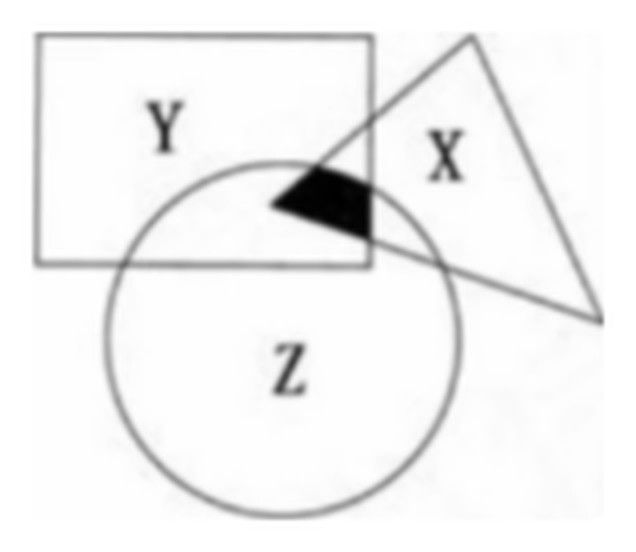
\includegraphics[width=0.20\textwidth]{figures/venn_XYZ_overlap.png}
\end{center}

\ifanswer
\solbegin
\step{设阴影部分的面积是 $x$，则 $290=64+180+160-24-70-36+x$，}
\step{$290=274+x$，$x=16$，故阴影部分的面积是 $16$.}
\solend

\fi

\item 如果集合 $A=\{1,2,3,\cdots,8\}$ 的子集 $B$ 满足：若 $2k\in B$，$k\in\N^{*}$，则 $2k+1\in B$，则称 $B$ 为 $A$ 的“好子集”，$A$ 的“好子集”有 \blankline[2.4em] 个.

\ifanswer
\solbegin
\step{由“好子集”定义得 $2$，$3$ 同时出现，$4$，$5$ 同时出现，$6$，$7$ 同时出现，}
\step{①当集合 $B$ 为空集时，满足题意；}
% 注：原卷此行印作「非空真子集共有 $2^4-1=15$ 种」，与同行算式冲突（$2^4-1=15$ 是**非空子集**数，
%     非空真子集应为 $2^4-2=14$），且与本段①（$B=\varnothing$）合起来恰构成「不含偶数的全体子集」，
%     故按文意订正为「非空子集」（段末总数 $1+15+24+12+2=54$ 不变）。
\step{②当集合 $B$ 中不存在偶数时，$\{1,3,5,7\}$ 的非空子集共有 $2^4-1=15$ 种；}
\step{③当集合 $B$ 中存在 $1$ 个偶数时，三个偶数中选择 $1$ 个，有 $C_3^1=3$ 种，}
\step{剩下 $3$ 个奇数不选，选 $1$ 个、$2$ 个、$3$ 个共有 $2^3=8$ 种，故共有 $24$ 种；}
\step{④当集合 $B$ 中存在 $2$ 个偶数时，三个偶数中选择 $2$ 个，有 $C_3^2=3$ 种，}
\step{剩下 $2$ 个奇数不选，选 $1$ 个、$2$ 个共有 $2^2=4$ 种，故共有 $12$ 种；}
\step{⑤当集合 $B$ 中存在 $3$ 个偶数时，三个偶数中选择 $3$ 个，有 $C_3^3=1$ 种，}
\step{剩下 $1$ 个奇数不选，选 $1$ 个共有 $2^1=2$ 种，故共有 $2$ 种；}
\step{所以 $A$ 的“好子集”共有 $1+15+24+12+2=54$ 种.}
\solend

\fi

\item 已知 $A=\{x\mid x=a^2-b^2,\ a\in\Z,b\in\Z,x\in\N^{*},x\leqslant 40\}$，则集合 $A$ 中共有 \blankline[2.4em] 个元素.

\ifanswer
\solbegin
\step{因为 $(k+1)^2-k^2=2k+1$，所以所有正奇数都属于集合 $A$，}
\step{又 $(2k+2)^2-(2k)^2=8k+4=4(2k+1)$，$(2k+1)^2-(2k-1)^2=8k=4\times 2k$，}
\step{因此所有 $4$ 的整数倍的正整数也属于 $A$，}
\step{若 $x=4k+2$，$k\in\N$，则 $a^2-b^2=(a+b)(a-b)=4k+2=2(2k+1)$，}
\step{则 $a+b$ 和 $a-b$ 中一定是一个取奇数，一个取偶数，}
\step{但是 $a,b\in\Z$ 时，$a+b$ 与 $a-b$ 同奇偶，所以此时无解，}
\step{即所有被 $4$ 除余 $2$ 的正整数都不属于 $A$，}
\step{所以每 $4$ 个数中，有 $3$ 个数属于集合 $A$，则集合 $A$ 中共含 $30$ 个元素.}
\solend

\fi

\item 十个元素组成的集合 $M=\{19,93,-1,0,25,-78,-94,1,17,-2\}$，$M$ 的所有非空子集记为 $M_i$（$i=1,2,\cdots,1023$），每一非空子集中所有元素的乘积记为 $m_i$（$i=1,2,\cdots,1023$），则 $m_1+m_2+\cdots+m_{1023}=$ \blankline[3em].

\ifanswer
\solbegin
\step{因为 $M$ 的所有非空子集为 $M_i$（$i=1,2,\cdots,1023$），这 $1023$ 个子集分成以下几种情况：}
\step{①含 $0$ 的子集有 $512$ 个，这些子集均满足 $m_i=0$；}
\step{②不含 $0$，含 $-1$ 且还含有其它元素的子集有 $255$ 个，}
\step{③不含 $0$，不含 $-1$ 但含有其它元素的子集有 $255$ 个，}
\step{④只含 $-1$ 的子集一个 $\{-1\}$，满足 $m_i=-1$；}
\step{其中②③中的集合是一一对应的，且满足 $m_i$ 对应成相反数，}
\step{故 $m_1+m_2+m_3+\cdots+m_{1023}=512\times 0+255\times 0-1=-1$.}
\solend

\fi

\item 已知 $M=\{(x,y)\mid |xy|=a\}$，$N=\{(x,y)\mid |xy|+1=|x|+|y|\}$，若集合 $M\cap N$ 中的点恰是正八边形的 $8$ 个顶点，则 $a=$ \blankline[2.4em].

\begin{center}
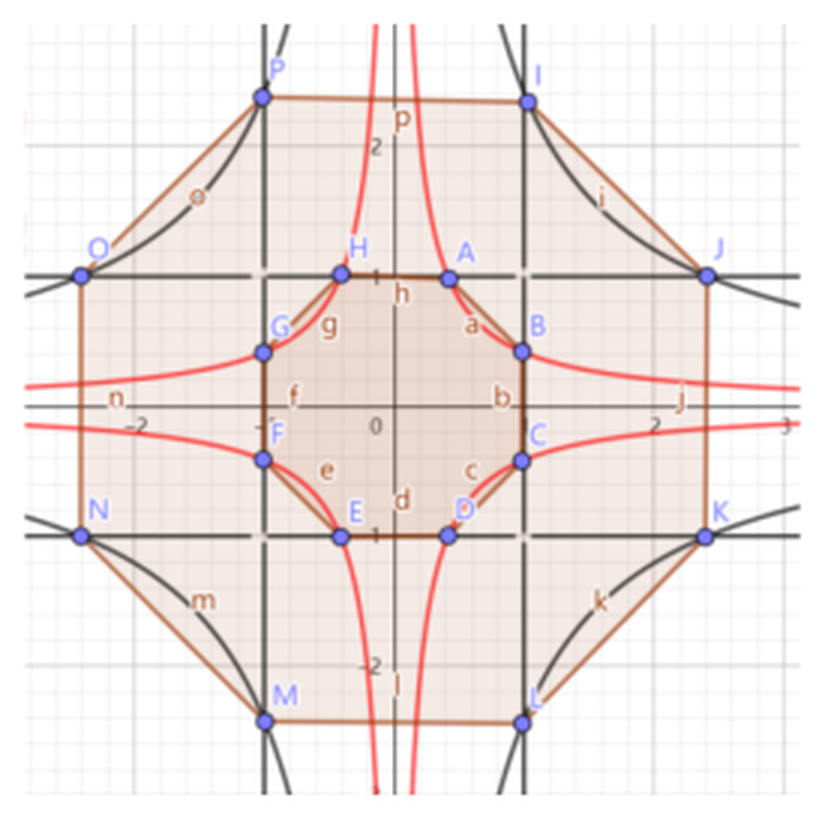
\includegraphics[width=0.44\textwidth]{figures/hyperbola_octagon.png}
\end{center}

\ifanswer
\solbegin
\step{$|xy|=a$ 和 $|xy|+1=|x|+|y|$ 的图像关于坐标轴均对称，只需考虑第一象限即可，}
\step{当 $x>0$，$y>0$ 时，$|xy|+1=|x|+|y|$ 即 $xy+1=x+y$，}
\step{即 $(x-1)(y-1)=0$，}
\step{即 $x=1$ 或 $y=1$，由对称性，作出完整的图像，}
\step{对于 $|xy|=a$，为四段双曲线，}
\step{考虑点 $A(I)(a,1)$，$B(J)(1,a)$，$C(K)(1,-a)$，}
\step{由 $AB=AC$ 得 $\sqrt{(a-1)^2+(1-a)^2}=2a$，解得 $a=\sqrt{2}\pm 1$.}
\solend

\fi

\item 集合 $A$ 是 $\{1,2,3,\cdots,100\}$ 的子集，若 $x\in A$，则 $2x\notin A$，$A$ 中的元素最多有 \blankline[2.4em] 个.

\ifanswer
\solbegin
\step{显然 $51$ 到 $100$ 共 $50$ 个可以，那么从 $1$ 到 $25$ 再 $2$ 倍不会超过 $50$，}
\step{$1$ 到 $25$ 中所有奇数都可以放到子集中，共有 $13$ 个，}
\step{再看偶数，$24=2\times 12$，$22=2\times 11$，$20=2\times 10$，$18=2\times 9$，$16=2\times 8$，}
% 注：末行照原卷抄录。原卷上一行列出 5 个偶数（24、22、20、18、16）而结论写「共有 $50+13+4=67$」，
%     此处的 $4$ 应作「另加 4 个元素」解（穷举验证集合 $A$ 的最大元素数确为 67），非笔误，故不改。
\step{及最后的 $4$，所以，共有 $50+13+4=67$.}
\solend

\fi

\end{enumerate}

\bigsec{二、选择题}

\begin{enumerate}
\setcounter{enumi}{13}

\item 下列各组集合中相等的是（\quad）.

①$P=\{x\mid x=2n,n\in\Z\}$，$Q=\{x\mid x=2(n-1),n\in\Z\}$；

②$P=\{x\mid x^2-1=0\}$，$Q=\left\{x\left|x=\dfrac{1+(-1)^n}{2},n\in\Z\right.\right\}$；

③$P=\{x\mid x=2m+1,m\in\Z\}$，$Q=\{x\mid x=4m\pm 1,m\in\Z\}$；

④$P=\{y\mid y=x^2+1\}$，$Q=\{x\mid y=x^2+1\}$.

\keepwithprev
A. ①②③④\qquad B. ①③\qquad C. ①②④\qquad D. ②④

\ans{B}

\item 如果一个命题的逆命题是真命题，那么这个命题的否命题是（\quad）

\keepwithprev
A. 真命题\qquad B. 假命题

C. 不一定是真命题\qquad D. 不一定是假命题

\ans{A}

\ifanswer
\solbegin
\step{一个命题的逆命题与这个命题的否命题是逆否命题，}
\step{它们的真假性相同，所以逆命题是真命题时，它们的否命题也是真命题. 故选 A.}
\solend

\fi

\item 设 $U$ 表示全集，下列命题中假命题有（\quad）

①若 $A\cap B=U$，则 $A=B=U$；②若 $A\cup B=\varnothing$，则 $A=B=\varnothing$；

③若 $A\cap B=\varnothing$，则 $\overline{A}\cup\overline{B}=U$；④若 $A\cup B=U$，则 $\overline{A}\cap\overline{B}=\varnothing$；

⑤若 $A\subseteq B$，则 $\overline{A}\supseteq\overline{B}$；⑥$\varnothing\in\{\varnothing\}$；⑦$\varnothing\subseteq\{\varnothing\}$.

\keepwithprev
A. $0$\qquad B. $1$\qquad C. $2$\qquad D. $3$

\ans{A}

\ifanswer
\solbegin
\step{全部正确，故选 A.}
\solend

\fi

\end{enumerate}

\bigsec{三、解答题}

\begin{enumerate}
\setcounter{enumi}{16}

\item 已知集合 $A=\{x\mid x^2-3x+2=0\}$，$B=\{x\mid x^2-bx+b-1=0\}$，$C=\{x\mid x^2-cx+2=0\}$.

\begin{enumerate}[label=(\arabic*)]
\item 若 $A\cup B=A$，求实数 $b$ 的值；
\item 若 $A\cap C=C$，求实数 $c$ 的取值范围.
\end{enumerate}

\ifanswer
\solbegin
\stepm{(1)}{$A=\{1,2\}$，$B=\{x\mid(x-1)(x-b+1)=0\}$，}
\step{由 $A\cup B=A$ 得 $b-1=1$ 或 $b-1=2$，所以 $b=2$ 或 $b=3$.}
\stepm{(2)}{由 $A\cap C=C$ 得 $C\subseteq A$，则 $C=\varnothing$ 或 $C=\{1\}$ 或 $C=\{2\}$ 或 $C=\{1,2\}$，}
\step{若 $C=\varnothing$，则 $\Delta=c^2-8<0$，解得 $-2\sqrt{2}<c<2\sqrt{2}$；}
\step{若 $C=\{1\}$，则 $\begin{cases}1+1=c\\ 1\times 1=2\end{cases}$，不可能；}
\step{若 $C=\{2\}$，则 $\begin{cases}2+2=c\\ 2\times 2=2\end{cases}$，不可能；}
\step{若 $C=\{1,2\}$，则 $\begin{cases}1+2=c\\ 1\times 2=2\end{cases}$，符合题意，$c=3$.}
\step{综上所述，$-2\sqrt{2}<c<2\sqrt{2}$ 或 $c=3$.}
\solend

\fi

\ansspace[6]

\item 已知全集 $U=\R$，$A=\{x\mid x^2+px+12=0\}$，$B=\{x\mid x^2-5x+q=0\}$，$\overline{A}\cap B=\{2\}$，求 $p+q$ 的值.

\ifanswer
\solbegin
\step{因为 $\overline{A}\cap B=\{2\}$，所以 $2\in B$，$2\notin A$，}
\step{所以 $2^2-5\times 2+q=0$，解得 $q=6$，$B=\{2,3\}$，}
\step{因为 $\overline{A}\cap B=\{2\}$，$B=\{2,3\}$，所以 $3\in A$，}
\step{所以 $3^2+p\times 3+12=0$，所以 $p=-7$，所以 $p+q=-1$.}
\solend

\fi

\ansspace[5]

\item 求证：方程 $x^2-abx+a+b=0$，$x^2-(a+b)x+ab=0$，其中 $a>2$，$b>2$ 没有公共根.

\ifanswer
\solbegin
\step{假设这两个方程有公共根 $\alpha$，则 $\alpha^2-ab\alpha+(a+b)=0$，$\alpha^2-(a+b)\alpha+ab=0$，}
\step{两式相减得 $(ab-a-b)(\alpha+1)=0$，}
\step{因为 $a>2$，$b>2$，所以 $a-1>1$，$b-1>1$，所以 $(a-1)(b-1)>1$，}
\step{所以 $ab-a-b>0$，所以 $\alpha+1=0$，所以 $\alpha=-1$，}
\step{代入第一个方程，得 $1+ab+a+b=0$，即 $(a+1)(b+1)=0$，}
\step{因为 $a>2$，$b>2$，所以该式不成立，所以这两个方程没有公共根.}
\solend

\fi

\ansspace[9]

% 压轴题：其后已无内容，故作答区全用可丢弃胶水（\ansspace*），并在题目前先量一下版面。
\ansneed{7cm}

\item 若集合 $A$ 具有以下性质：①$0\in A$，$1\in A$；②若 $x$、$y\in A$，则 $x-y\in A$，且 $x\neq 0$ 时，$\dfrac{1}{x}\in A$；则称集合 $A$ 是“好集”.

\begin{enumerate}[label=(\arabic*)]
\item 分别判断集合 $B=\{-1,0,1\}$，有理数集 $\Q$ 是否是“好集”，并说明理由；
\item 设集合 $A$ 是“好集”，求证：若 $x$、$y\in A$，则 $x+y\in A$；
\item 对任意的一个“好集” $A$，分别判断下面命题的真假，并说明理由.

命题 $p$：若 $x$、$y\in A$，则必有 $xy\in A$；

命题 $q$：若 $x$、$y\in A$，且 $x\neq 0$，则必有 $\dfrac{y}{x}\in A$.
\end{enumerate}

\ifanswer
\solbegin
\stepm{(1)}{集合 $B$ 不是“好集”. 理由是：假设集合 $B$ 是“好集”.}
\step{因为 $-1\in B$，$1\in B$，所以 $-1-1=-2\in B$. 这与 $-2\notin B$ 矛盾.}
\step{有理数集 $\Q$ 是“好集”. 因为 $0\in\Q$，$1\in\Q$，}
\step{对任意的 $x$、$y\in\Q$，有 $x-y\in\Q$，且 $x\neq 0$ 时，$\dfrac{1}{x}\in\Q$，}
\step{所以有理数集 $\Q$ 是“好集”.}
\stepm{(2)}{因为集合 $A$ 是“好集”，所以 $0\in A$.}
\step{若 $x$、$y\in A$，则 $0-y\in A$，即 $-y\in A$，所以 $x-(-y)\in A$，即 $x+y\in A$.}
\stepm{(3)}{命题 $p$、$q$ 均为真命题. 理由如下：}
\step{对任意一个“好集” $A$，任取 $x$、$y\in A$，}
\step{若 $x$、$y$ 中有 $0$ 或 $1$ 时，显然 $xy\in A$.}
\step{下设 $x$、$y$ 均不为 $0$，$1$. 由定义得 $x-1$，$\dfrac{1}{x-1}$，$\dfrac{1}{x}\in A$，}
\step{所以 $\dfrac{1}{x-1}-\dfrac{1}{x}\in A$，即 $\dfrac{1}{x(x-1)}\in A$，所以 $x(x-1)\in A$.}
\step{由（2）得 $x(x-1)+x\in A$，即 $x^2\in A$. 同理可得 $y^2\in A$.}
\step{若 $x+y=0$ 或 $x+y=1$，则 $x^2+y^2\in A$.}
\step{若 $x+y\neq 0$ 且 $x+y\neq 1$，则 $(x+y)^2\in A$，}
\step{所以 $2xy=(x+y)^2-x^2-y^2\in A$，所以 $\dfrac{1}{2xy}\in A$，}
\step{由（2）得 $\dfrac{1}{xy}=\dfrac{1}{2xy}+\dfrac{1}{2xy}\in A$，所以 $xy\in A$.}
\step{综上，$xy\in A$，即命题 $p$ 为真命题.}
\step{若 $x$、$y\in A$，且 $x\neq 0$，则 $\dfrac{1}{x}\in A$，}
\step{所以 $\dfrac{y}{x}=y\cdot\dfrac{1}{x}\in A$，即命题 $q$ 为真命题.}
\solend

\fi

\ansspace*[11]

\end{enumerate}

\end{document}
"
% 紧凑版：xelatex "\def\iscompact{1}% 高一14_华师大二附中_集合与逻辑单元练习.tex
%   —— 高一上数学「2026-2027 年华师大二附中高一上 集合与逻辑单元练习」（试卷版/答案版）
% 试卷版：xelatex 高一14_华师大二附中_集合与逻辑单元练习.tex
% 答案版：xelatex "\def\isanswer{1}\input{高一14_华师大二附中_集合与逻辑单元练习.tex}"
% 紧凑版：xelatex "\def\iscompact{1}\input{高一14_华师大二附中_集合与逻辑单元练习.tex}"
%
% 原始材料是微信公众号图文（「魔都数学加油站」），正文为 6 张 PNG 页（1080×1527）。
% 原文本身就是一份**讲评版**——题目下方直接印出【答案】或【解析】，选择题更是把答案
% 直接印在括注里（第 14 题）。试题文字、答案与解析均照原卷录入，未改内容。卷面上的
% 粉色斜水印「魔都数学加油站」属水印，未录入。
%
% 与原卷的排版差异（均已在 README「说明」中交代）：
%   ① 原文自**第 3 题**起（第 1、2 题未在该文中发布），故本稿题号亦自 3 起；
%   ② 原卷未印分节标题，本稿按题型补出「一、填空题」「二、选择题」「三、解答题」三节；
%   ③ 原卷填空、选择题的答案直接印在题目下方（第 14 题印在括注里），本稿统一改为
%      试卷版隐去、答案版以【答案】或【解析】给出，使两版彻底分离；
%   ④ 原卷的 $\R$、$\Q$、$\Z$、$\N$、$\N^{*}$ 时作正体 $R$、$Q$、$Z$、$N$、$N^*$，
%      本稿按全稿惯例统一写作 $\R$、$\Q$、$\Z$、$\N$、$\N^{*}$；
%   ⑤ 原卷中文括注用**半角**括号（第 4 题「(填“真”或“假”)」、第 15 题「是(  )」、
%      第 16 题「有(    )」，均已放大核实），本稿按全稿惯例排全角；
%   ⑥ 第 3 题题干作「$a$ 为**指定**实数」、同题解析作「$a$ 为**给定**的实数」，二者同义，
%      本稿两处均照原卷抄录（未统一）。

% 原卷笔误一处（已逐处放大到能看清字形后核对，本稿按文意订正，并在 README 中写明原委）：
%   ① 第 9 题【解析】② 原卷印「$\{1,3,5,7\}$ 的非空**真**子集共有 $2^4-1=15$ 种」，
%      与同行算式冲突（$2^4-1=15$ 是**非空子集**数，非空真子集应为 $2^4-2=14$），
%      且与本段①（$B=\varnothing$）合起来恰构成「不含偶数的全体子集」，故订正为「非空子集」，
%      段末总数 $1+15+24+12+2=54$ 不变。
%
% 原卷存疑一处（无法确证原意，本稿照抄并加 % 注）：
%   ① 第 12 题【解析】末行「由 $AB=AC$ 得 $\sqrt{(a-1)^2+(1-a)^2}=2a$，解得 $a=\sqrt2\pm1$」——
%      按此式只能解出 $a=\sqrt2-1$（$a=\sqrt2+1$ 处左端 $2$、右端 $4.83$，等式不成立），
%      而其答案 $a=\sqrt2\pm1$ 经数值验证是正确的（两值互为倒数，均使 $M\cap N$ 的 8 个交点按
%      $45^\circ$ 均布）。疑为解析此式笔误，但无法确证原意，本稿照抄原卷、未改。
%      同行上一行的「考虑点 $A(I)(a,1)$，$B(J)(1,a)$，$C(K)(1,-a)$」（点标 I/J/K 与
%      figures/hyperbola_octagon.png 中的标注一一对应）与本行等号右端的 $2a$，均照原卷录入；
%      2026-09-15 回原图逐处放大复核时发现曾误作 $A(1,a)$、$B(a,1)$、$C(-1,a)$ 与「$=2$」，
%      已按原卷订正（见 README「高一14—高一18 专记」）。

\documentclass[a4paper,11pt]{article}
\usepackage{common}

\begin{document}

\examtitlest[3]{2026--2027 年华师大二附中高一上}{集合与逻辑单元练习}

\bigsec{一、填空题}

\begin{enumerate}
\setcounter{enumi}{2}

\item 已知 $a$ 为指定实数，$M=\{x\mid x^2-3x-a^2+2=0\}$ 的非空真子集个数是 \blankline[2.4em].

\ifanswer
\solbegin
\step{集合 $M=\{x\mid x^2-3x-a^2+2=0\}$，$a$ 为给定的实数，}
\step{关于方程 $x^2-3x-a^2+2=0$，因为 $\Delta=(-3)^2-4(2-a^2)=4a^2+1>0$，}
\step{所以方程有两个不同的实根，所以 $M$ 中有两个元素，}
\step{所以集合 $M$ 的非空真子集的个数为 $2^2-2=2$.}
\solend

\fi

\item 判断下列命题的真假：（填“真”或“假”）

（1）任何集合都不是空集的子集 \blankline[2.4em]；

（2）一个有理数与一个无理数的和与积都是无理数 \blankline[2.4em]；

（3）如果一个整数 $n$ 的平方是偶数，那么 $n$ 是偶数 \blankline[2.4em].

\ans{假，假，真}

\item 请写出“如果两个三角形全等，那么它们的面积相等”的逆否命题：\blankline[3em].

\ifanswer
\solbegin
\step{如果两个三角形的面积不相等，则这两个三角形不全等.}
\solend

\fi

\item 已知 $U=\{(x,y)\mid x,y\in\R\}$，$M=\left\{(x,y)\left|\dfrac{y-2}{x-1}=3\right.\right\}$，$N=\{(x,y)\mid y=3x-1\}$，$\overline{M}\cap N=$ \blankline[3em].

\ans{$\{(1,2)\}$}

\item 已知集合 $A=\{x\mid 5x-a\leqslant 0\}$，$B=\{x\mid 6x-b>0\}$，$a$、$b\in\N$，且 $A\cap B\cap\N=\{2,3,4\}$，则整数对 $(a,b)$ 的个数为 \blankline[2.4em].

\ifanswer
\solbegin
\step{$A=\left\{x\left|x\leqslant\dfrac{a}{5}\right.\right\}$，$B=\left\{x\left|x>\dfrac{b}{6}\right.\right\}$，因为 $A\cap B\cap\N=\{2,3,4\}$，}
\step{所以 $4\leqslant\dfrac{a}{5}<5$，$1\leqslant\dfrac{b}{6}<2$，解得 $20\leqslant a<25$，$6\leqslant b<12$，}
\step{又 $a$、$b\in\N$，所以 $a=20$，$21$，$22$，$23$，$24$，$b=6$，$7$，$8$，$9$，$10$，$11$，}
\step{则整数对 $(a,b)$ 的个数为 $30$.}
\solend

\fi

\item 如图所示，$X$、$Y$、$Z$ 分别是面积为 $64$、$180$、$160$ 的三张不同形状的纸片，它们部分重叠放在一起盖在桌面上，总共盖住的面积为 $290$，且 $X$ 与 $Y$、$Y$ 与 $Z$、$Z$ 与 $X$ 重叠部分面积分别为 $24$、$70$、$36$，问阴影部分的面积是 \blankline[2.4em].

\begin{center}
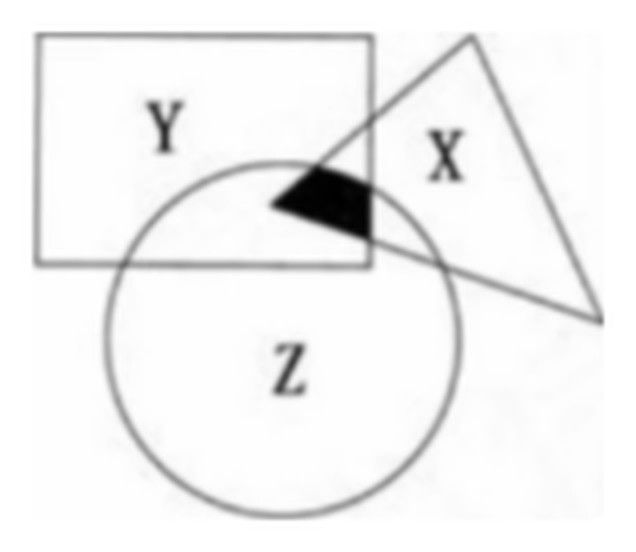
\includegraphics[width=0.20\textwidth]{figures/venn_XYZ_overlap.png}
\end{center}

\ifanswer
\solbegin
\step{设阴影部分的面积是 $x$，则 $290=64+180+160-24-70-36+x$，}
\step{$290=274+x$，$x=16$，故阴影部分的面积是 $16$.}
\solend

\fi

\item 如果集合 $A=\{1,2,3,\cdots,8\}$ 的子集 $B$ 满足：若 $2k\in B$，$k\in\N^{*}$，则 $2k+1\in B$，则称 $B$ 为 $A$ 的“好子集”，$A$ 的“好子集”有 \blankline[2.4em] 个.

\ifanswer
\solbegin
\step{由“好子集”定义得 $2$，$3$ 同时出现，$4$，$5$ 同时出现，$6$，$7$ 同时出现，}
\step{①当集合 $B$ 为空集时，满足题意；}
% 注：原卷此行印作「非空真子集共有 $2^4-1=15$ 种」，与同行算式冲突（$2^4-1=15$ 是**非空子集**数，
%     非空真子集应为 $2^4-2=14$），且与本段①（$B=\varnothing$）合起来恰构成「不含偶数的全体子集」，
%     故按文意订正为「非空子集」（段末总数 $1+15+24+12+2=54$ 不变）。
\step{②当集合 $B$ 中不存在偶数时，$\{1,3,5,7\}$ 的非空子集共有 $2^4-1=15$ 种；}
\step{③当集合 $B$ 中存在 $1$ 个偶数时，三个偶数中选择 $1$ 个，有 $C_3^1=3$ 种，}
\step{剩下 $3$ 个奇数不选，选 $1$ 个、$2$ 个、$3$ 个共有 $2^3=8$ 种，故共有 $24$ 种；}
\step{④当集合 $B$ 中存在 $2$ 个偶数时，三个偶数中选择 $2$ 个，有 $C_3^2=3$ 种，}
\step{剩下 $2$ 个奇数不选，选 $1$ 个、$2$ 个共有 $2^2=4$ 种，故共有 $12$ 种；}
\step{⑤当集合 $B$ 中存在 $3$ 个偶数时，三个偶数中选择 $3$ 个，有 $C_3^3=1$ 种，}
\step{剩下 $1$ 个奇数不选，选 $1$ 个共有 $2^1=2$ 种，故共有 $2$ 种；}
\step{所以 $A$ 的“好子集”共有 $1+15+24+12+2=54$ 种.}
\solend

\fi

\item 已知 $A=\{x\mid x=a^2-b^2,\ a\in\Z,b\in\Z,x\in\N^{*},x\leqslant 40\}$，则集合 $A$ 中共有 \blankline[2.4em] 个元素.

\ifanswer
\solbegin
\step{因为 $(k+1)^2-k^2=2k+1$，所以所有正奇数都属于集合 $A$，}
\step{又 $(2k+2)^2-(2k)^2=8k+4=4(2k+1)$，$(2k+1)^2-(2k-1)^2=8k=4\times 2k$，}
\step{因此所有 $4$ 的整数倍的正整数也属于 $A$，}
\step{若 $x=4k+2$，$k\in\N$，则 $a^2-b^2=(a+b)(a-b)=4k+2=2(2k+1)$，}
\step{则 $a+b$ 和 $a-b$ 中一定是一个取奇数，一个取偶数，}
\step{但是 $a,b\in\Z$ 时，$a+b$ 与 $a-b$ 同奇偶，所以此时无解，}
\step{即所有被 $4$ 除余 $2$ 的正整数都不属于 $A$，}
\step{所以每 $4$ 个数中，有 $3$ 个数属于集合 $A$，则集合 $A$ 中共含 $30$ 个元素.}
\solend

\fi

\item 十个元素组成的集合 $M=\{19,93,-1,0,25,-78,-94,1,17,-2\}$，$M$ 的所有非空子集记为 $M_i$（$i=1,2,\cdots,1023$），每一非空子集中所有元素的乘积记为 $m_i$（$i=1,2,\cdots,1023$），则 $m_1+m_2+\cdots+m_{1023}=$ \blankline[3em].

\ifanswer
\solbegin
\step{因为 $M$ 的所有非空子集为 $M_i$（$i=1,2,\cdots,1023$），这 $1023$ 个子集分成以下几种情况：}
\step{①含 $0$ 的子集有 $512$ 个，这些子集均满足 $m_i=0$；}
\step{②不含 $0$，含 $-1$ 且还含有其它元素的子集有 $255$ 个，}
\step{③不含 $0$，不含 $-1$ 但含有其它元素的子集有 $255$ 个，}
\step{④只含 $-1$ 的子集一个 $\{-1\}$，满足 $m_i=-1$；}
\step{其中②③中的集合是一一对应的，且满足 $m_i$ 对应成相反数，}
\step{故 $m_1+m_2+m_3+\cdots+m_{1023}=512\times 0+255\times 0-1=-1$.}
\solend

\fi

\item 已知 $M=\{(x,y)\mid |xy|=a\}$，$N=\{(x,y)\mid |xy|+1=|x|+|y|\}$，若集合 $M\cap N$ 中的点恰是正八边形的 $8$ 个顶点，则 $a=$ \blankline[2.4em].

\begin{center}
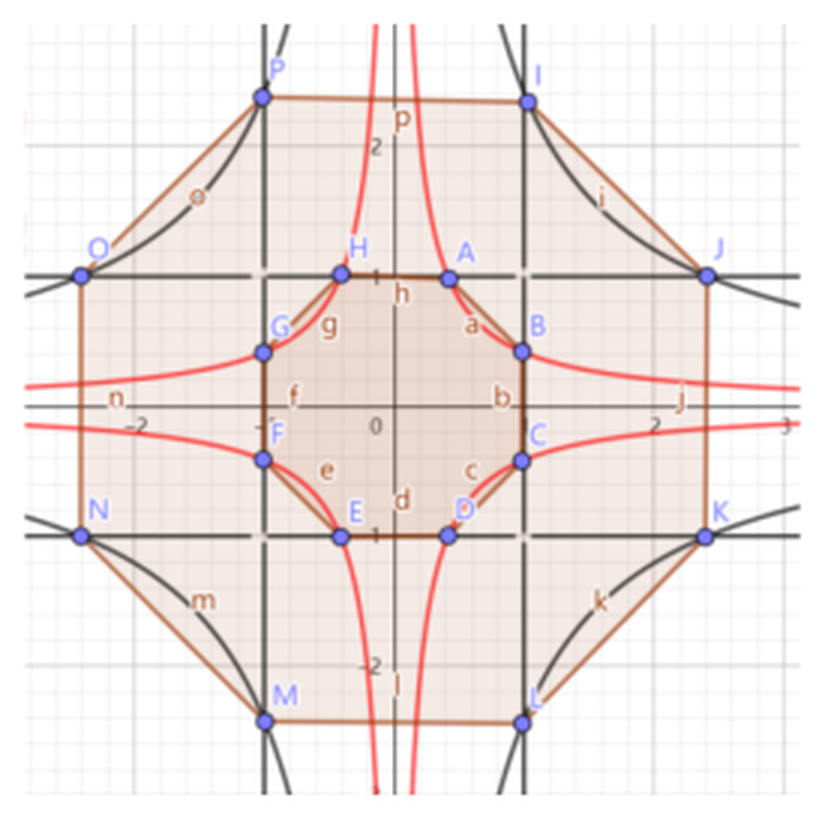
\includegraphics[width=0.44\textwidth]{figures/hyperbola_octagon.png}
\end{center}

\ifanswer
\solbegin
\step{$|xy|=a$ 和 $|xy|+1=|x|+|y|$ 的图像关于坐标轴均对称，只需考虑第一象限即可，}
\step{当 $x>0$，$y>0$ 时，$|xy|+1=|x|+|y|$ 即 $xy+1=x+y$，}
\step{即 $(x-1)(y-1)=0$，}
\step{即 $x=1$ 或 $y=1$，由对称性，作出完整的图像，}
\step{对于 $|xy|=a$，为四段双曲线，}
\step{考虑点 $A(I)(a,1)$，$B(J)(1,a)$，$C(K)(1,-a)$，}
\step{由 $AB=AC$ 得 $\sqrt{(a-1)^2+(1-a)^2}=2a$，解得 $a=\sqrt{2}\pm 1$.}
\solend

\fi

\item 集合 $A$ 是 $\{1,2,3,\cdots,100\}$ 的子集，若 $x\in A$，则 $2x\notin A$，$A$ 中的元素最多有 \blankline[2.4em] 个.

\ifanswer
\solbegin
\step{显然 $51$ 到 $100$ 共 $50$ 个可以，那么从 $1$ 到 $25$ 再 $2$ 倍不会超过 $50$，}
\step{$1$ 到 $25$ 中所有奇数都可以放到子集中，共有 $13$ 个，}
\step{再看偶数，$24=2\times 12$，$22=2\times 11$，$20=2\times 10$，$18=2\times 9$，$16=2\times 8$，}
% 注：末行照原卷抄录。原卷上一行列出 5 个偶数（24、22、20、18、16）而结论写「共有 $50+13+4=67$」，
%     此处的 $4$ 应作「另加 4 个元素」解（穷举验证集合 $A$ 的最大元素数确为 67），非笔误，故不改。
\step{及最后的 $4$，所以，共有 $50+13+4=67$.}
\solend

\fi

\end{enumerate}

\bigsec{二、选择题}

\begin{enumerate}
\setcounter{enumi}{13}

\item 下列各组集合中相等的是（\quad）.

①$P=\{x\mid x=2n,n\in\Z\}$，$Q=\{x\mid x=2(n-1),n\in\Z\}$；

②$P=\{x\mid x^2-1=0\}$，$Q=\left\{x\left|x=\dfrac{1+(-1)^n}{2},n\in\Z\right.\right\}$；

③$P=\{x\mid x=2m+1,m\in\Z\}$，$Q=\{x\mid x=4m\pm 1,m\in\Z\}$；

④$P=\{y\mid y=x^2+1\}$，$Q=\{x\mid y=x^2+1\}$.

\keepwithprev
A. ①②③④\qquad B. ①③\qquad C. ①②④\qquad D. ②④

\ans{B}

\item 如果一个命题的逆命题是真命题，那么这个命题的否命题是（\quad）

\keepwithprev
A. 真命题\qquad B. 假命题

C. 不一定是真命题\qquad D. 不一定是假命题

\ans{A}

\ifanswer
\solbegin
\step{一个命题的逆命题与这个命题的否命题是逆否命题，}
\step{它们的真假性相同，所以逆命题是真命题时，它们的否命题也是真命题. 故选 A.}
\solend

\fi

\item 设 $U$ 表示全集，下列命题中假命题有（\quad）

①若 $A\cap B=U$，则 $A=B=U$；②若 $A\cup B=\varnothing$，则 $A=B=\varnothing$；

③若 $A\cap B=\varnothing$，则 $\overline{A}\cup\overline{B}=U$；④若 $A\cup B=U$，则 $\overline{A}\cap\overline{B}=\varnothing$；

⑤若 $A\subseteq B$，则 $\overline{A}\supseteq\overline{B}$；⑥$\varnothing\in\{\varnothing\}$；⑦$\varnothing\subseteq\{\varnothing\}$.

\keepwithprev
A. $0$\qquad B. $1$\qquad C. $2$\qquad D. $3$

\ans{A}

\ifanswer
\solbegin
\step{全部正确，故选 A.}
\solend

\fi

\end{enumerate}

\bigsec{三、解答题}

\begin{enumerate}
\setcounter{enumi}{16}

\item 已知集合 $A=\{x\mid x^2-3x+2=0\}$，$B=\{x\mid x^2-bx+b-1=0\}$，$C=\{x\mid x^2-cx+2=0\}$.

\begin{enumerate}[label=(\arabic*)]
\item 若 $A\cup B=A$，求实数 $b$ 的值；
\item 若 $A\cap C=C$，求实数 $c$ 的取值范围.
\end{enumerate}

\ifanswer
\solbegin
\stepm{(1)}{$A=\{1,2\}$，$B=\{x\mid(x-1)(x-b+1)=0\}$，}
\step{由 $A\cup B=A$ 得 $b-1=1$ 或 $b-1=2$，所以 $b=2$ 或 $b=3$.}
\stepm{(2)}{由 $A\cap C=C$ 得 $C\subseteq A$，则 $C=\varnothing$ 或 $C=\{1\}$ 或 $C=\{2\}$ 或 $C=\{1,2\}$，}
\step{若 $C=\varnothing$，则 $\Delta=c^2-8<0$，解得 $-2\sqrt{2}<c<2\sqrt{2}$；}
\step{若 $C=\{1\}$，则 $\begin{cases}1+1=c\\ 1\times 1=2\end{cases}$，不可能；}
\step{若 $C=\{2\}$，则 $\begin{cases}2+2=c\\ 2\times 2=2\end{cases}$，不可能；}
\step{若 $C=\{1,2\}$，则 $\begin{cases}1+2=c\\ 1\times 2=2\end{cases}$，符合题意，$c=3$.}
\step{综上所述，$-2\sqrt{2}<c<2\sqrt{2}$ 或 $c=3$.}
\solend

\fi

\ansspace[6]

\item 已知全集 $U=\R$，$A=\{x\mid x^2+px+12=0\}$，$B=\{x\mid x^2-5x+q=0\}$，$\overline{A}\cap B=\{2\}$，求 $p+q$ 的值.

\ifanswer
\solbegin
\step{因为 $\overline{A}\cap B=\{2\}$，所以 $2\in B$，$2\notin A$，}
\step{所以 $2^2-5\times 2+q=0$，解得 $q=6$，$B=\{2,3\}$，}
\step{因为 $\overline{A}\cap B=\{2\}$，$B=\{2,3\}$，所以 $3\in A$，}
\step{所以 $3^2+p\times 3+12=0$，所以 $p=-7$，所以 $p+q=-1$.}
\solend

\fi

\ansspace[5]

\item 求证：方程 $x^2-abx+a+b=0$，$x^2-(a+b)x+ab=0$，其中 $a>2$，$b>2$ 没有公共根.

\ifanswer
\solbegin
\step{假设这两个方程有公共根 $\alpha$，则 $\alpha^2-ab\alpha+(a+b)=0$，$\alpha^2-(a+b)\alpha+ab=0$，}
\step{两式相减得 $(ab-a-b)(\alpha+1)=0$，}
\step{因为 $a>2$，$b>2$，所以 $a-1>1$，$b-1>1$，所以 $(a-1)(b-1)>1$，}
\step{所以 $ab-a-b>0$，所以 $\alpha+1=0$，所以 $\alpha=-1$，}
\step{代入第一个方程，得 $1+ab+a+b=0$，即 $(a+1)(b+1)=0$，}
\step{因为 $a>2$，$b>2$，所以该式不成立，所以这两个方程没有公共根.}
\solend

\fi

\ansspace[9]

% 压轴题：其后已无内容，故作答区全用可丢弃胶水（\ansspace*），并在题目前先量一下版面。
\ansneed{7cm}

\item 若集合 $A$ 具有以下性质：①$0\in A$，$1\in A$；②若 $x$、$y\in A$，则 $x-y\in A$，且 $x\neq 0$ 时，$\dfrac{1}{x}\in A$；则称集合 $A$ 是“好集”.

\begin{enumerate}[label=(\arabic*)]
\item 分别判断集合 $B=\{-1,0,1\}$，有理数集 $\Q$ 是否是“好集”，并说明理由；
\item 设集合 $A$ 是“好集”，求证：若 $x$、$y\in A$，则 $x+y\in A$；
\item 对任意的一个“好集” $A$，分别判断下面命题的真假，并说明理由.

命题 $p$：若 $x$、$y\in A$，则必有 $xy\in A$；

命题 $q$：若 $x$、$y\in A$，且 $x\neq 0$，则必有 $\dfrac{y}{x}\in A$.
\end{enumerate}

\ifanswer
\solbegin
\stepm{(1)}{集合 $B$ 不是“好集”. 理由是：假设集合 $B$ 是“好集”.}
\step{因为 $-1\in B$，$1\in B$，所以 $-1-1=-2\in B$. 这与 $-2\notin B$ 矛盾.}
\step{有理数集 $\Q$ 是“好集”. 因为 $0\in\Q$，$1\in\Q$，}
\step{对任意的 $x$、$y\in\Q$，有 $x-y\in\Q$，且 $x\neq 0$ 时，$\dfrac{1}{x}\in\Q$，}
\step{所以有理数集 $\Q$ 是“好集”.}
\stepm{(2)}{因为集合 $A$ 是“好集”，所以 $0\in A$.}
\step{若 $x$、$y\in A$，则 $0-y\in A$，即 $-y\in A$，所以 $x-(-y)\in A$，即 $x+y\in A$.}
\stepm{(3)}{命题 $p$、$q$ 均为真命题. 理由如下：}
\step{对任意一个“好集” $A$，任取 $x$、$y\in A$，}
\step{若 $x$、$y$ 中有 $0$ 或 $1$ 时，显然 $xy\in A$.}
\step{下设 $x$、$y$ 均不为 $0$，$1$. 由定义得 $x-1$，$\dfrac{1}{x-1}$，$\dfrac{1}{x}\in A$，}
\step{所以 $\dfrac{1}{x-1}-\dfrac{1}{x}\in A$，即 $\dfrac{1}{x(x-1)}\in A$，所以 $x(x-1)\in A$.}
\step{由（2）得 $x(x-1)+x\in A$，即 $x^2\in A$. 同理可得 $y^2\in A$.}
\step{若 $x+y=0$ 或 $x+y=1$，则 $x^2+y^2\in A$.}
\step{若 $x+y\neq 0$ 且 $x+y\neq 1$，则 $(x+y)^2\in A$，}
\step{所以 $2xy=(x+y)^2-x^2-y^2\in A$，所以 $\dfrac{1}{2xy}\in A$，}
\step{由（2）得 $\dfrac{1}{xy}=\dfrac{1}{2xy}+\dfrac{1}{2xy}\in A$，所以 $xy\in A$.}
\step{综上，$xy\in A$，即命题 $p$ 为真命题.}
\step{若 $x$、$y\in A$，且 $x\neq 0$，则 $\dfrac{1}{x}\in A$，}
\step{所以 $\dfrac{y}{x}=y\cdot\dfrac{1}{x}\in A$，即命题 $q$ 为真命题.}
\solend

\fi

\ansspace*[11]

\end{enumerate}

\end{document}
"
%
% 原始材料是微信公众号图文（「魔都数学加油站」），正文为 6 张 PNG 页（1080×1527）。
% 原文本身就是一份**讲评版**——题目下方直接印出【答案】或【解析】，选择题更是把答案
% 直接印在括注里（第 14 题）。试题文字、答案与解析均照原卷录入，未改内容。卷面上的
% 粉色斜水印「魔都数学加油站」属水印，未录入。
%
% 与原卷的排版差异（均已在 README「说明」中交代）：
%   ① 原文自**第 3 题**起（第 1、2 题未在该文中发布），故本稿题号亦自 3 起；
%   ② 原卷未印分节标题，本稿按题型补出「一、填空题」「二、选择题」「三、解答题」三节；
%   ③ 原卷填空、选择题的答案直接印在题目下方（第 14 题印在括注里），本稿统一改为
%      试卷版隐去、答案版以【答案】或【解析】给出，使两版彻底分离；
%   ④ 原卷的 $\R$、$\Q$、$\Z$、$\N$、$\N^{*}$ 时作正体 $R$、$Q$、$Z$、$N$、$N^*$，
%      本稿按全稿惯例统一写作 $\R$、$\Q$、$\Z$、$\N$、$\N^{*}$；
%   ⑤ 原卷中文括注用**半角**括号（第 4 题「(填“真”或“假”)」、第 15 题「是(  )」、
%      第 16 题「有(    )」，均已放大核实），本稿按全稿惯例排全角；
%   ⑥ 第 3 题题干作「$a$ 为**指定**实数」、同题解析作「$a$ 为**给定**的实数」，二者同义，
%      本稿两处均照原卷抄录（未统一）。

% 原卷笔误一处（已逐处放大到能看清字形后核对，本稿按文意订正，并在 README 中写明原委）：
%   ① 第 9 题【解析】② 原卷印「$\{1,3,5,7\}$ 的非空**真**子集共有 $2^4-1=15$ 种」，
%      与同行算式冲突（$2^4-1=15$ 是**非空子集**数，非空真子集应为 $2^4-2=14$），
%      且与本段①（$B=\varnothing$）合起来恰构成「不含偶数的全体子集」，故订正为「非空子集」，
%      段末总数 $1+15+24+12+2=54$ 不变。
%
% 原卷存疑一处（无法确证原意，本稿照抄并加 % 注）：
%   ① 第 12 题【解析】末行「由 $AB=AC$ 得 $\sqrt{(a-1)^2+(1-a)^2}=2a$，解得 $a=\sqrt2\pm1$」——
%      按此式只能解出 $a=\sqrt2-1$（$a=\sqrt2+1$ 处左端 $2$、右端 $4.83$，等式不成立），
%      而其答案 $a=\sqrt2\pm1$ 经数值验证是正确的（两值互为倒数，均使 $M\cap N$ 的 8 个交点按
%      $45^\circ$ 均布）。疑为解析此式笔误，但无法确证原意，本稿照抄原卷、未改。
%      同行上一行的「考虑点 $A(I)(a,1)$，$B(J)(1,a)$，$C(K)(1,-a)$」（点标 I/J/K 与
%      figures/hyperbola_octagon.png 中的标注一一对应）与本行等号右端的 $2a$，均照原卷录入；
%      2026-09-15 回原图逐处放大复核时发现曾误作 $A(1,a)$、$B(a,1)$、$C(-1,a)$ 与「$=2$」，
%      已按原卷订正（见 README「高一14—高一18 专记」）。

\documentclass[a4paper,11pt]{article}
\usepackage{common}

\begin{document}

\examtitlest[3]{2026--2027 年华师大二附中高一上}{集合与逻辑单元练习}

\bigsec{一、填空题}

\begin{enumerate}
\setcounter{enumi}{2}

\item 已知 $a$ 为指定实数，$M=\{x\mid x^2-3x-a^2+2=0\}$ 的非空真子集个数是 \blankline[2.4em].

\ifanswer
\solbegin
\step{集合 $M=\{x\mid x^2-3x-a^2+2=0\}$，$a$ 为给定的实数，}
\step{关于方程 $x^2-3x-a^2+2=0$，因为 $\Delta=(-3)^2-4(2-a^2)=4a^2+1>0$，}
\step{所以方程有两个不同的实根，所以 $M$ 中有两个元素，}
\step{所以集合 $M$ 的非空真子集的个数为 $2^2-2=2$.}
\solend

\fi

\item 判断下列命题的真假：（填“真”或“假”）

（1）任何集合都不是空集的子集 \blankline[2.4em]；

（2）一个有理数与一个无理数的和与积都是无理数 \blankline[2.4em]；

（3）如果一个整数 $n$ 的平方是偶数，那么 $n$ 是偶数 \blankline[2.4em].

\ans{假，假，真}

\item 请写出“如果两个三角形全等，那么它们的面积相等”的逆否命题：\blankline[3em].

\ifanswer
\solbegin
\step{如果两个三角形的面积不相等，则这两个三角形不全等.}
\solend

\fi

\item 已知 $U=\{(x,y)\mid x,y\in\R\}$，$M=\left\{(x,y)\left|\dfrac{y-2}{x-1}=3\right.\right\}$，$N=\{(x,y)\mid y=3x-1\}$，$\overline{M}\cap N=$ \blankline[3em].

\ans{$\{(1,2)\}$}

\item 已知集合 $A=\{x\mid 5x-a\leqslant 0\}$，$B=\{x\mid 6x-b>0\}$，$a$、$b\in\N$，且 $A\cap B\cap\N=\{2,3,4\}$，则整数对 $(a,b)$ 的个数为 \blankline[2.4em].

\ifanswer
\solbegin
\step{$A=\left\{x\left|x\leqslant\dfrac{a}{5}\right.\right\}$，$B=\left\{x\left|x>\dfrac{b}{6}\right.\right\}$，因为 $A\cap B\cap\N=\{2,3,4\}$，}
\step{所以 $4\leqslant\dfrac{a}{5}<5$，$1\leqslant\dfrac{b}{6}<2$，解得 $20\leqslant a<25$，$6\leqslant b<12$，}
\step{又 $a$、$b\in\N$，所以 $a=20$，$21$，$22$，$23$，$24$，$b=6$，$7$，$8$，$9$，$10$，$11$，}
\step{则整数对 $(a,b)$ 的个数为 $30$.}
\solend

\fi

\item 如图所示，$X$、$Y$、$Z$ 分别是面积为 $64$、$180$、$160$ 的三张不同形状的纸片，它们部分重叠放在一起盖在桌面上，总共盖住的面积为 $290$，且 $X$ 与 $Y$、$Y$ 与 $Z$、$Z$ 与 $X$ 重叠部分面积分别为 $24$、$70$、$36$，问阴影部分的面积是 \blankline[2.4em].

\begin{center}
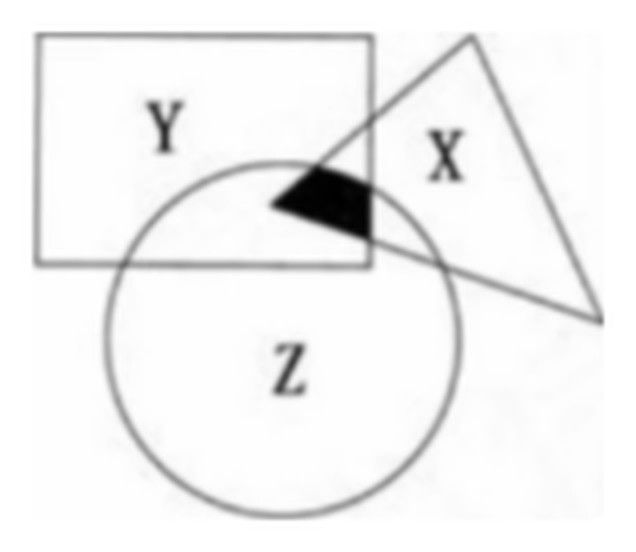
\includegraphics[width=0.20\textwidth]{figures/venn_XYZ_overlap.png}
\end{center}

\ifanswer
\solbegin
\step{设阴影部分的面积是 $x$，则 $290=64+180+160-24-70-36+x$，}
\step{$290=274+x$，$x=16$，故阴影部分的面积是 $16$.}
\solend

\fi

\item 如果集合 $A=\{1,2,3,\cdots,8\}$ 的子集 $B$ 满足：若 $2k\in B$，$k\in\N^{*}$，则 $2k+1\in B$，则称 $B$ 为 $A$ 的“好子集”，$A$ 的“好子集”有 \blankline[2.4em] 个.

\ifanswer
\solbegin
\step{由“好子集”定义得 $2$，$3$ 同时出现，$4$，$5$ 同时出现，$6$，$7$ 同时出现，}
\step{①当集合 $B$ 为空集时，满足题意；}
% 注：原卷此行印作「非空真子集共有 $2^4-1=15$ 种」，与同行算式冲突（$2^4-1=15$ 是**非空子集**数，
%     非空真子集应为 $2^4-2=14$），且与本段①（$B=\varnothing$）合起来恰构成「不含偶数的全体子集」，
%     故按文意订正为「非空子集」（段末总数 $1+15+24+12+2=54$ 不变）。
\step{②当集合 $B$ 中不存在偶数时，$\{1,3,5,7\}$ 的非空子集共有 $2^4-1=15$ 种；}
\step{③当集合 $B$ 中存在 $1$ 个偶数时，三个偶数中选择 $1$ 个，有 $C_3^1=3$ 种，}
\step{剩下 $3$ 个奇数不选，选 $1$ 个、$2$ 个、$3$ 个共有 $2^3=8$ 种，故共有 $24$ 种；}
\step{④当集合 $B$ 中存在 $2$ 个偶数时，三个偶数中选择 $2$ 个，有 $C_3^2=3$ 种，}
\step{剩下 $2$ 个奇数不选，选 $1$ 个、$2$ 个共有 $2^2=4$ 种，故共有 $12$ 种；}
\step{⑤当集合 $B$ 中存在 $3$ 个偶数时，三个偶数中选择 $3$ 个，有 $C_3^3=1$ 种，}
\step{剩下 $1$ 个奇数不选，选 $1$ 个共有 $2^1=2$ 种，故共有 $2$ 种；}
\step{所以 $A$ 的“好子集”共有 $1+15+24+12+2=54$ 种.}
\solend

\fi

\item 已知 $A=\{x\mid x=a^2-b^2,\ a\in\Z,b\in\Z,x\in\N^{*},x\leqslant 40\}$，则集合 $A$ 中共有 \blankline[2.4em] 个元素.

\ifanswer
\solbegin
\step{因为 $(k+1)^2-k^2=2k+1$，所以所有正奇数都属于集合 $A$，}
\step{又 $(2k+2)^2-(2k)^2=8k+4=4(2k+1)$，$(2k+1)^2-(2k-1)^2=8k=4\times 2k$，}
\step{因此所有 $4$ 的整数倍的正整数也属于 $A$，}
\step{若 $x=4k+2$，$k\in\N$，则 $a^2-b^2=(a+b)(a-b)=4k+2=2(2k+1)$，}
\step{则 $a+b$ 和 $a-b$ 中一定是一个取奇数，一个取偶数，}
\step{但是 $a,b\in\Z$ 时，$a+b$ 与 $a-b$ 同奇偶，所以此时无解，}
\step{即所有被 $4$ 除余 $2$ 的正整数都不属于 $A$，}
\step{所以每 $4$ 个数中，有 $3$ 个数属于集合 $A$，则集合 $A$ 中共含 $30$ 个元素.}
\solend

\fi

\item 十个元素组成的集合 $M=\{19,93,-1,0,25,-78,-94,1,17,-2\}$，$M$ 的所有非空子集记为 $M_i$（$i=1,2,\cdots,1023$），每一非空子集中所有元素的乘积记为 $m_i$（$i=1,2,\cdots,1023$），则 $m_1+m_2+\cdots+m_{1023}=$ \blankline[3em].

\ifanswer
\solbegin
\step{因为 $M$ 的所有非空子集为 $M_i$（$i=1,2,\cdots,1023$），这 $1023$ 个子集分成以下几种情况：}
\step{①含 $0$ 的子集有 $512$ 个，这些子集均满足 $m_i=0$；}
\step{②不含 $0$，含 $-1$ 且还含有其它元素的子集有 $255$ 个，}
\step{③不含 $0$，不含 $-1$ 但含有其它元素的子集有 $255$ 个，}
\step{④只含 $-1$ 的子集一个 $\{-1\}$，满足 $m_i=-1$；}
\step{其中②③中的集合是一一对应的，且满足 $m_i$ 对应成相反数，}
\step{故 $m_1+m_2+m_3+\cdots+m_{1023}=512\times 0+255\times 0-1=-1$.}
\solend

\fi

\item 已知 $M=\{(x,y)\mid |xy|=a\}$，$N=\{(x,y)\mid |xy|+1=|x|+|y|\}$，若集合 $M\cap N$ 中的点恰是正八边形的 $8$ 个顶点，则 $a=$ \blankline[2.4em].

\begin{center}
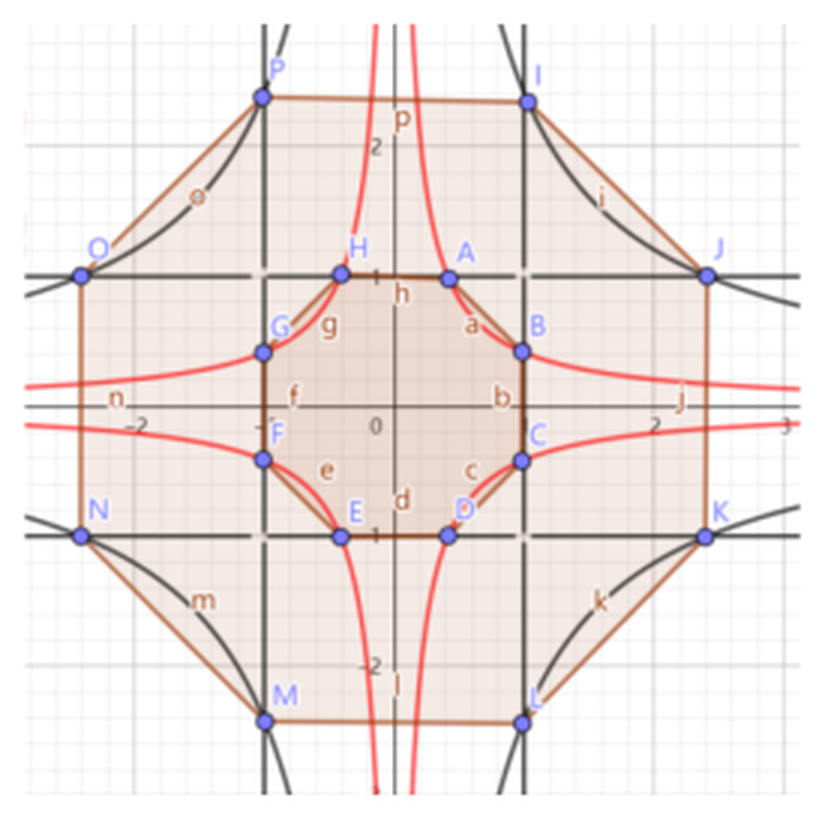
\includegraphics[width=0.44\textwidth]{figures/hyperbola_octagon.png}
\end{center}

\ifanswer
\solbegin
\step{$|xy|=a$ 和 $|xy|+1=|x|+|y|$ 的图像关于坐标轴均对称，只需考虑第一象限即可，}
\step{当 $x>0$，$y>0$ 时，$|xy|+1=|x|+|y|$ 即 $xy+1=x+y$，}
\step{即 $(x-1)(y-1)=0$，}
\step{即 $x=1$ 或 $y=1$，由对称性，作出完整的图像，}
\step{对于 $|xy|=a$，为四段双曲线，}
\step{考虑点 $A(I)(a,1)$，$B(J)(1,a)$，$C(K)(1,-a)$，}
\step{由 $AB=AC$ 得 $\sqrt{(a-1)^2+(1-a)^2}=2a$，解得 $a=\sqrt{2}\pm 1$.}
\solend

\fi

\item 集合 $A$ 是 $\{1,2,3,\cdots,100\}$ 的子集，若 $x\in A$，则 $2x\notin A$，$A$ 中的元素最多有 \blankline[2.4em] 个.

\ifanswer
\solbegin
\step{显然 $51$ 到 $100$ 共 $50$ 个可以，那么从 $1$ 到 $25$ 再 $2$ 倍不会超过 $50$，}
\step{$1$ 到 $25$ 中所有奇数都可以放到子集中，共有 $13$ 个，}
\step{再看偶数，$24=2\times 12$，$22=2\times 11$，$20=2\times 10$，$18=2\times 9$，$16=2\times 8$，}
% 注：末行照原卷抄录。原卷上一行列出 5 个偶数（24、22、20、18、16）而结论写「共有 $50+13+4=67$」，
%     此处的 $4$ 应作「另加 4 个元素」解（穷举验证集合 $A$ 的最大元素数确为 67），非笔误，故不改。
\step{及最后的 $4$，所以，共有 $50+13+4=67$.}
\solend

\fi

\end{enumerate}

\bigsec{二、选择题}

\begin{enumerate}
\setcounter{enumi}{13}

\item 下列各组集合中相等的是（\quad）.

①$P=\{x\mid x=2n,n\in\Z\}$，$Q=\{x\mid x=2(n-1),n\in\Z\}$；

②$P=\{x\mid x^2-1=0\}$，$Q=\left\{x\left|x=\dfrac{1+(-1)^n}{2},n\in\Z\right.\right\}$；

③$P=\{x\mid x=2m+1,m\in\Z\}$，$Q=\{x\mid x=4m\pm 1,m\in\Z\}$；

④$P=\{y\mid y=x^2+1\}$，$Q=\{x\mid y=x^2+1\}$.

\keepwithprev
A. ①②③④\qquad B. ①③\qquad C. ①②④\qquad D. ②④

\ans{B}

\item 如果一个命题的逆命题是真命题，那么这个命题的否命题是（\quad）

\keepwithprev
A. 真命题\qquad B. 假命题

C. 不一定是真命题\qquad D. 不一定是假命题

\ans{A}

\ifanswer
\solbegin
\step{一个命题的逆命题与这个命题的否命题是逆否命题，}
\step{它们的真假性相同，所以逆命题是真命题时，它们的否命题也是真命题. 故选 A.}
\solend

\fi

\item 设 $U$ 表示全集，下列命题中假命题有（\quad）

①若 $A\cap B=U$，则 $A=B=U$；②若 $A\cup B=\varnothing$，则 $A=B=\varnothing$；

③若 $A\cap B=\varnothing$，则 $\overline{A}\cup\overline{B}=U$；④若 $A\cup B=U$，则 $\overline{A}\cap\overline{B}=\varnothing$；

⑤若 $A\subseteq B$，则 $\overline{A}\supseteq\overline{B}$；⑥$\varnothing\in\{\varnothing\}$；⑦$\varnothing\subseteq\{\varnothing\}$.

\keepwithprev
A. $0$\qquad B. $1$\qquad C. $2$\qquad D. $3$

\ans{A}

\ifanswer
\solbegin
\step{全部正确，故选 A.}
\solend

\fi

\end{enumerate}

\bigsec{三、解答题}

\begin{enumerate}
\setcounter{enumi}{16}

\item 已知集合 $A=\{x\mid x^2-3x+2=0\}$，$B=\{x\mid x^2-bx+b-1=0\}$，$C=\{x\mid x^2-cx+2=0\}$.

\begin{enumerate}[label=(\arabic*)]
\item 若 $A\cup B=A$，求实数 $b$ 的值；
\item 若 $A\cap C=C$，求实数 $c$ 的取值范围.
\end{enumerate}

\ifanswer
\solbegin
\stepm{(1)}{$A=\{1,2\}$，$B=\{x\mid(x-1)(x-b+1)=0\}$，}
\step{由 $A\cup B=A$ 得 $b-1=1$ 或 $b-1=2$，所以 $b=2$ 或 $b=3$.}
\stepm{(2)}{由 $A\cap C=C$ 得 $C\subseteq A$，则 $C=\varnothing$ 或 $C=\{1\}$ 或 $C=\{2\}$ 或 $C=\{1,2\}$，}
\step{若 $C=\varnothing$，则 $\Delta=c^2-8<0$，解得 $-2\sqrt{2}<c<2\sqrt{2}$；}
\step{若 $C=\{1\}$，则 $\begin{cases}1+1=c\\ 1\times 1=2\end{cases}$，不可能；}
\step{若 $C=\{2\}$，则 $\begin{cases}2+2=c\\ 2\times 2=2\end{cases}$，不可能；}
\step{若 $C=\{1,2\}$，则 $\begin{cases}1+2=c\\ 1\times 2=2\end{cases}$，符合题意，$c=3$.}
\step{综上所述，$-2\sqrt{2}<c<2\sqrt{2}$ 或 $c=3$.}
\solend

\fi

\ansspace[6]

\item 已知全集 $U=\R$，$A=\{x\mid x^2+px+12=0\}$，$B=\{x\mid x^2-5x+q=0\}$，$\overline{A}\cap B=\{2\}$，求 $p+q$ 的值.

\ifanswer
\solbegin
\step{因为 $\overline{A}\cap B=\{2\}$，所以 $2\in B$，$2\notin A$，}
\step{所以 $2^2-5\times 2+q=0$，解得 $q=6$，$B=\{2,3\}$，}
\step{因为 $\overline{A}\cap B=\{2\}$，$B=\{2,3\}$，所以 $3\in A$，}
\step{所以 $3^2+p\times 3+12=0$，所以 $p=-7$，所以 $p+q=-1$.}
\solend

\fi

\ansspace[5]

\item 求证：方程 $x^2-abx+a+b=0$，$x^2-(a+b)x+ab=0$，其中 $a>2$，$b>2$ 没有公共根.

\ifanswer
\solbegin
\step{假设这两个方程有公共根 $\alpha$，则 $\alpha^2-ab\alpha+(a+b)=0$，$\alpha^2-(a+b)\alpha+ab=0$，}
\step{两式相减得 $(ab-a-b)(\alpha+1)=0$，}
\step{因为 $a>2$，$b>2$，所以 $a-1>1$，$b-1>1$，所以 $(a-1)(b-1)>1$，}
\step{所以 $ab-a-b>0$，所以 $\alpha+1=0$，所以 $\alpha=-1$，}
\step{代入第一个方程，得 $1+ab+a+b=0$，即 $(a+1)(b+1)=0$，}
\step{因为 $a>2$，$b>2$，所以该式不成立，所以这两个方程没有公共根.}
\solend

\fi

\ansspace[9]

% 压轴题：其后已无内容，故作答区全用可丢弃胶水（\ansspace*），并在题目前先量一下版面。
\ansneed{7cm}

\item 若集合 $A$ 具有以下性质：①$0\in A$，$1\in A$；②若 $x$、$y\in A$，则 $x-y\in A$，且 $x\neq 0$ 时，$\dfrac{1}{x}\in A$；则称集合 $A$ 是“好集”.

\begin{enumerate}[label=(\arabic*)]
\item 分别判断集合 $B=\{-1,0,1\}$，有理数集 $\Q$ 是否是“好集”，并说明理由；
\item 设集合 $A$ 是“好集”，求证：若 $x$、$y\in A$，则 $x+y\in A$；
\item 对任意的一个“好集” $A$，分别判断下面命题的真假，并说明理由.

命题 $p$：若 $x$、$y\in A$，则必有 $xy\in A$；

命题 $q$：若 $x$、$y\in A$，且 $x\neq 0$，则必有 $\dfrac{y}{x}\in A$.
\end{enumerate}

\ifanswer
\solbegin
\stepm{(1)}{集合 $B$ 不是“好集”. 理由是：假设集合 $B$ 是“好集”.}
\step{因为 $-1\in B$，$1\in B$，所以 $-1-1=-2\in B$. 这与 $-2\notin B$ 矛盾.}
\step{有理数集 $\Q$ 是“好集”. 因为 $0\in\Q$，$1\in\Q$，}
\step{对任意的 $x$、$y\in\Q$，有 $x-y\in\Q$，且 $x\neq 0$ 时，$\dfrac{1}{x}\in\Q$，}
\step{所以有理数集 $\Q$ 是“好集”.}
\stepm{(2)}{因为集合 $A$ 是“好集”，所以 $0\in A$.}
\step{若 $x$、$y\in A$，则 $0-y\in A$，即 $-y\in A$，所以 $x-(-y)\in A$，即 $x+y\in A$.}
\stepm{(3)}{命题 $p$、$q$ 均为真命题. 理由如下：}
\step{对任意一个“好集” $A$，任取 $x$、$y\in A$，}
\step{若 $x$、$y$ 中有 $0$ 或 $1$ 时，显然 $xy\in A$.}
\step{下设 $x$、$y$ 均不为 $0$，$1$. 由定义得 $x-1$，$\dfrac{1}{x-1}$，$\dfrac{1}{x}\in A$，}
\step{所以 $\dfrac{1}{x-1}-\dfrac{1}{x}\in A$，即 $\dfrac{1}{x(x-1)}\in A$，所以 $x(x-1)\in A$.}
\step{由（2）得 $x(x-1)+x\in A$，即 $x^2\in A$. 同理可得 $y^2\in A$.}
\step{若 $x+y=0$ 或 $x+y=1$，则 $x^2+y^2\in A$.}
\step{若 $x+y\neq 0$ 且 $x+y\neq 1$，则 $(x+y)^2\in A$，}
\step{所以 $2xy=(x+y)^2-x^2-y^2\in A$，所以 $\dfrac{1}{2xy}\in A$，}
\step{由（2）得 $\dfrac{1}{xy}=\dfrac{1}{2xy}+\dfrac{1}{2xy}\in A$，所以 $xy\in A$.}
\step{综上，$xy\in A$，即命题 $p$ 为真命题.}
\step{若 $x$、$y\in A$，且 $x\neq 0$，则 $\dfrac{1}{x}\in A$，}
\step{所以 $\dfrac{y}{x}=y\cdot\dfrac{1}{x}\in A$，即命题 $q$ 为真命题.}
\solend

\fi

\ansspace*[11]

\end{enumerate}

\end{document}
"
%
% 原始材料是微信公众号图文（「魔都数学加油站」），正文为 6 张 PNG 页（1080×1527）。
% 原文本身就是一份**讲评版**——题目下方直接印出【答案】或【解析】，选择题更是把答案
% 直接印在括注里（第 14 题）。试题文字、答案与解析均照原卷录入，未改内容。卷面上的
% 粉色斜水印「魔都数学加油站」属水印，未录入。
%
% 与原卷的排版差异（均已在 README「说明」中交代）：
%   ① 原文自**第 3 题**起（第 1、2 题未在该文中发布），故本稿题号亦自 3 起；
%   ② 原卷未印分节标题，本稿按题型补出「一、填空题」「二、选择题」「三、解答题」三节；
%   ③ 原卷填空、选择题的答案直接印在题目下方（第 14 题印在括注里），本稿统一改为
%      试卷版隐去、答案版以【答案】或【解析】给出，使两版彻底分离；
%   ④ 原卷的 $\R$、$\Q$、$\Z$、$\N$、$\N^{*}$ 时作正体 $R$、$Q$、$Z$、$N$、$N^*$，
%      本稿按全稿惯例统一写作 $\R$、$\Q$、$\Z$、$\N$、$\N^{*}$；
%   ⑤ 原卷中文括注用**半角**括号（第 4 题「(填“真”或“假”)」、第 15 题「是(  )」、
%      第 16 题「有(    )」，均已放大核实），本稿按全稿惯例排全角；
%   ⑥ 第 3 题题干作「$a$ 为**指定**实数」、同题解析作「$a$ 为**给定**的实数」，二者同义，
%      本稿两处均照原卷抄录（未统一）。

% 原卷笔误一处（已逐处放大到能看清字形后核对，本稿按文意订正，并在 README 中写明原委）：
%   ① 第 9 题【解析】② 原卷印「$\{1,3,5,7\}$ 的非空**真**子集共有 $2^4-1=15$ 种」，
%      与同行算式冲突（$2^4-1=15$ 是**非空子集**数，非空真子集应为 $2^4-2=14$），
%      且与本段①（$B=\varnothing$）合起来恰构成「不含偶数的全体子集」，故订正为「非空子集」，
%      段末总数 $1+15+24+12+2=54$ 不变。
%
% 原卷存疑一处（无法确证原意，本稿照抄并加 % 注）：
%   ① 第 12 题【解析】末行「由 $AB=AC$ 得 $\sqrt{(a-1)^2+(1-a)^2}=2a$，解得 $a=\sqrt2\pm1$」——
%      按此式只能解出 $a=\sqrt2-1$（$a=\sqrt2+1$ 处左端 $2$、右端 $4.83$，等式不成立），
%      而其答案 $a=\sqrt2\pm1$ 经数值验证是正确的（两值互为倒数，均使 $M\cap N$ 的 8 个交点按
%      $45^\circ$ 均布）。疑为解析此式笔误，但无法确证原意，本稿照抄原卷、未改。
%      同行上一行的「考虑点 $A(I)(a,1)$，$B(J)(1,a)$，$C(K)(1,-a)$」（点标 I/J/K 与
%      figures/hyperbola_octagon.png 中的标注一一对应）与本行等号右端的 $2a$，均照原卷录入；
%      2026-09-15 回原图逐处放大复核时发现曾误作 $A(1,a)$、$B(a,1)$、$C(-1,a)$ 与「$=2$」，
%      已按原卷订正（见 README「高一14—高一18 专记」）。

\documentclass[a4paper,11pt]{article}
\usepackage{common}

\begin{document}

\examtitlest[3]{2026--2027 年华师大二附中高一上}{集合与逻辑单元练习}

\bigsec{一、填空题}

\begin{enumerate}
\setcounter{enumi}{2}

\item 已知 $a$ 为指定实数，$M=\{x\mid x^2-3x-a^2+2=0\}$ 的非空真子集个数是 \blankline[2.4em].

\ifanswer
\solbegin
\step{集合 $M=\{x\mid x^2-3x-a^2+2=0\}$，$a$ 为给定的实数，}
\step{关于方程 $x^2-3x-a^2+2=0$，因为 $\Delta=(-3)^2-4(2-a^2)=4a^2+1>0$，}
\step{所以方程有两个不同的实根，所以 $M$ 中有两个元素，}
\step{所以集合 $M$ 的非空真子集的个数为 $2^2-2=2$.}
\solend

\fi

\item 判断下列命题的真假：（填“真”或“假”）

（1）任何集合都不是空集的子集 \blankline[2.4em]；

（2）一个有理数与一个无理数的和与积都是无理数 \blankline[2.4em]；

（3）如果一个整数 $n$ 的平方是偶数，那么 $n$ 是偶数 \blankline[2.4em].

\ans{假，假，真}

\item 请写出“如果两个三角形全等，那么它们的面积相等”的逆否命题：\blankline[3em].

\ifanswer
\solbegin
\step{如果两个三角形的面积不相等，则这两个三角形不全等.}
\solend

\fi

\item 已知 $U=\{(x,y)\mid x,y\in\R\}$，$M=\left\{(x,y)\left|\dfrac{y-2}{x-1}=3\right.\right\}$，$N=\{(x,y)\mid y=3x-1\}$，$\overline{M}\cap N=$ \blankline[3em].

\ans{$\{(1,2)\}$}

\item 已知集合 $A=\{x\mid 5x-a\leqslant 0\}$，$B=\{x\mid 6x-b>0\}$，$a$、$b\in\N$，且 $A\cap B\cap\N=\{2,3,4\}$，则整数对 $(a,b)$ 的个数为 \blankline[2.4em].

\ifanswer
\solbegin
\step{$A=\left\{x\left|x\leqslant\dfrac{a}{5}\right.\right\}$，$B=\left\{x\left|x>\dfrac{b}{6}\right.\right\}$，因为 $A\cap B\cap\N=\{2,3,4\}$，}
\step{所以 $4\leqslant\dfrac{a}{5}<5$，$1\leqslant\dfrac{b}{6}<2$，解得 $20\leqslant a<25$，$6\leqslant b<12$，}
\step{又 $a$、$b\in\N$，所以 $a=20$，$21$，$22$，$23$，$24$，$b=6$，$7$，$8$，$9$，$10$，$11$，}
\step{则整数对 $(a,b)$ 的个数为 $30$.}
\solend

\fi

\item 如图所示，$X$、$Y$、$Z$ 分别是面积为 $64$、$180$、$160$ 的三张不同形状的纸片，它们部分重叠放在一起盖在桌面上，总共盖住的面积为 $290$，且 $X$ 与 $Y$、$Y$ 与 $Z$、$Z$ 与 $X$ 重叠部分面积分别为 $24$、$70$、$36$，问阴影部分的面积是 \blankline[2.4em].

\begin{center}
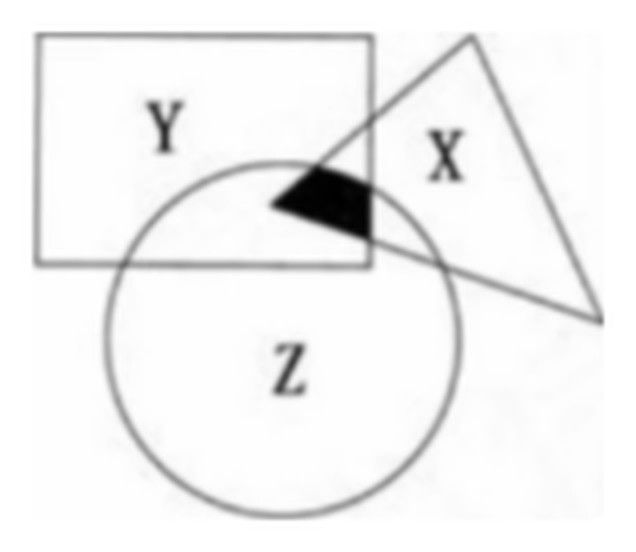
\includegraphics[width=0.20\textwidth]{figures/venn_XYZ_overlap.png}
\end{center}

\ifanswer
\solbegin
\step{设阴影部分的面积是 $x$，则 $290=64+180+160-24-70-36+x$，}
\step{$290=274+x$，$x=16$，故阴影部分的面积是 $16$.}
\solend

\fi

\item 如果集合 $A=\{1,2,3,\cdots,8\}$ 的子集 $B$ 满足：若 $2k\in B$，$k\in\N^{*}$，则 $2k+1\in B$，则称 $B$ 为 $A$ 的“好子集”，$A$ 的“好子集”有 \blankline[2.4em] 个.

\ifanswer
\solbegin
\step{由“好子集”定义得 $2$，$3$ 同时出现，$4$，$5$ 同时出现，$6$，$7$ 同时出现，}
\step{①当集合 $B$ 为空集时，满足题意；}
% 注：原卷此行印作「非空真子集共有 $2^4-1=15$ 种」，与同行算式冲突（$2^4-1=15$ 是**非空子集**数，
%     非空真子集应为 $2^4-2=14$），且与本段①（$B=\varnothing$）合起来恰构成「不含偶数的全体子集」，
%     故按文意订正为「非空子集」（段末总数 $1+15+24+12+2=54$ 不变）。
\step{②当集合 $B$ 中不存在偶数时，$\{1,3,5,7\}$ 的非空子集共有 $2^4-1=15$ 种；}
\step{③当集合 $B$ 中存在 $1$ 个偶数时，三个偶数中选择 $1$ 个，有 $C_3^1=3$ 种，}
\step{剩下 $3$ 个奇数不选，选 $1$ 个、$2$ 个、$3$ 个共有 $2^3=8$ 种，故共有 $24$ 种；}
\step{④当集合 $B$ 中存在 $2$ 个偶数时，三个偶数中选择 $2$ 个，有 $C_3^2=3$ 种，}
\step{剩下 $2$ 个奇数不选，选 $1$ 个、$2$ 个共有 $2^2=4$ 种，故共有 $12$ 种；}
\step{⑤当集合 $B$ 中存在 $3$ 个偶数时，三个偶数中选择 $3$ 个，有 $C_3^3=1$ 种，}
\step{剩下 $1$ 个奇数不选，选 $1$ 个共有 $2^1=2$ 种，故共有 $2$ 种；}
\step{所以 $A$ 的“好子集”共有 $1+15+24+12+2=54$ 种.}
\solend

\fi

\item 已知 $A=\{x\mid x=a^2-b^2,\ a\in\Z,b\in\Z,x\in\N^{*},x\leqslant 40\}$，则集合 $A$ 中共有 \blankline[2.4em] 个元素.

\ifanswer
\solbegin
\step{因为 $(k+1)^2-k^2=2k+1$，所以所有正奇数都属于集合 $A$，}
\step{又 $(2k+2)^2-(2k)^2=8k+4=4(2k+1)$，$(2k+1)^2-(2k-1)^2=8k=4\times 2k$，}
\step{因此所有 $4$ 的整数倍的正整数也属于 $A$，}
\step{若 $x=4k+2$，$k\in\N$，则 $a^2-b^2=(a+b)(a-b)=4k+2=2(2k+1)$，}
\step{则 $a+b$ 和 $a-b$ 中一定是一个取奇数，一个取偶数，}
\step{但是 $a,b\in\Z$ 时，$a+b$ 与 $a-b$ 同奇偶，所以此时无解，}
\step{即所有被 $4$ 除余 $2$ 的正整数都不属于 $A$，}
\step{所以每 $4$ 个数中，有 $3$ 个数属于集合 $A$，则集合 $A$ 中共含 $30$ 个元素.}
\solend

\fi

\item 十个元素组成的集合 $M=\{19,93,-1,0,25,-78,-94,1,17,-2\}$，$M$ 的所有非空子集记为 $M_i$（$i=1,2,\cdots,1023$），每一非空子集中所有元素的乘积记为 $m_i$（$i=1,2,\cdots,1023$），则 $m_1+m_2+\cdots+m_{1023}=$ \blankline[3em].

\ifanswer
\solbegin
\step{因为 $M$ 的所有非空子集为 $M_i$（$i=1,2,\cdots,1023$），这 $1023$ 个子集分成以下几种情况：}
\step{①含 $0$ 的子集有 $512$ 个，这些子集均满足 $m_i=0$；}
\step{②不含 $0$，含 $-1$ 且还含有其它元素的子集有 $255$ 个，}
\step{③不含 $0$，不含 $-1$ 但含有其它元素的子集有 $255$ 个，}
\step{④只含 $-1$ 的子集一个 $\{-1\}$，满足 $m_i=-1$；}
\step{其中②③中的集合是一一对应的，且满足 $m_i$ 对应成相反数，}
\step{故 $m_1+m_2+m_3+\cdots+m_{1023}=512\times 0+255\times 0-1=-1$.}
\solend

\fi

\item 已知 $M=\{(x,y)\mid |xy|=a\}$，$N=\{(x,y)\mid |xy|+1=|x|+|y|\}$，若集合 $M\cap N$ 中的点恰是正八边形的 $8$ 个顶点，则 $a=$ \blankline[2.4em].

\begin{center}
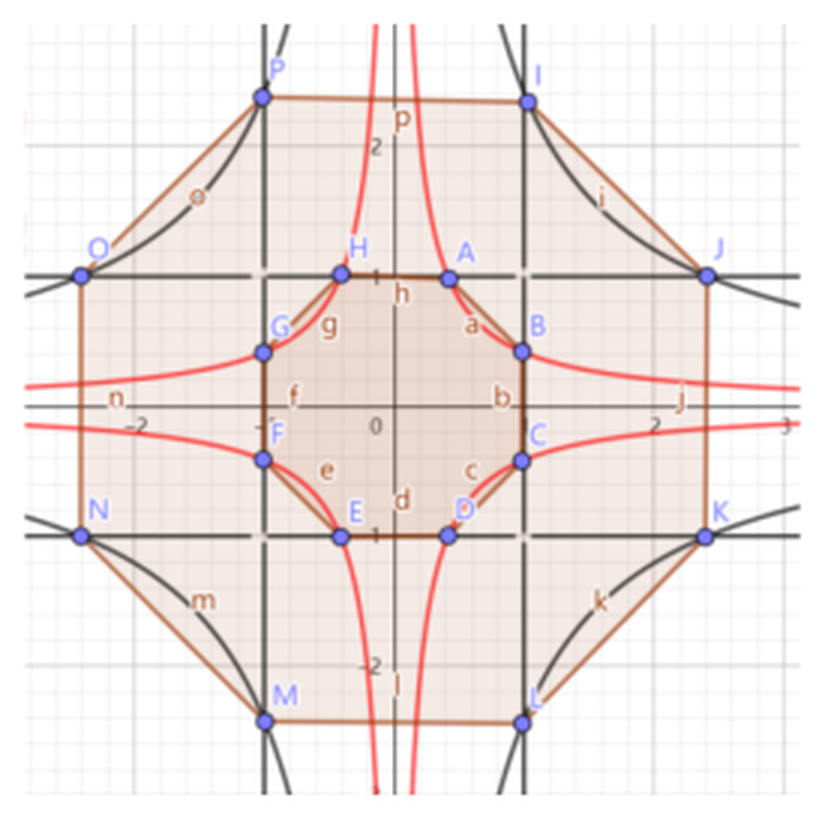
\includegraphics[width=0.44\textwidth]{figures/hyperbola_octagon.png}
\end{center}

\ifanswer
\solbegin
\step{$|xy|=a$ 和 $|xy|+1=|x|+|y|$ 的图像关于坐标轴均对称，只需考虑第一象限即可，}
\step{当 $x>0$，$y>0$ 时，$|xy|+1=|x|+|y|$ 即 $xy+1=x+y$，}
\step{即 $(x-1)(y-1)=0$，}
\step{即 $x=1$ 或 $y=1$，由对称性，作出完整的图像，}
\step{对于 $|xy|=a$，为四段双曲线，}
\step{考虑点 $A(I)(a,1)$，$B(J)(1,a)$，$C(K)(1,-a)$，}
\step{由 $AB=AC$ 得 $\sqrt{(a-1)^2+(1-a)^2}=2a$，解得 $a=\sqrt{2}\pm 1$.}
\solend

\fi

\item 集合 $A$ 是 $\{1,2,3,\cdots,100\}$ 的子集，若 $x\in A$，则 $2x\notin A$，$A$ 中的元素最多有 \blankline[2.4em] 个.

\ifanswer
\solbegin
\step{显然 $51$ 到 $100$ 共 $50$ 个可以，那么从 $1$ 到 $25$ 再 $2$ 倍不会超过 $50$，}
\step{$1$ 到 $25$ 中所有奇数都可以放到子集中，共有 $13$ 个，}
\step{再看偶数，$24=2\times 12$，$22=2\times 11$，$20=2\times 10$，$18=2\times 9$，$16=2\times 8$，}
% 注：末行照原卷抄录。原卷上一行列出 5 个偶数（24、22、20、18、16）而结论写「共有 $50+13+4=67$」，
%     此处的 $4$ 应作「另加 4 个元素」解（穷举验证集合 $A$ 的最大元素数确为 67），非笔误，故不改。
\step{及最后的 $4$，所以，共有 $50+13+4=67$.}
\solend

\fi

\end{enumerate}

\bigsec{二、选择题}

\begin{enumerate}
\setcounter{enumi}{13}

\item 下列各组集合中相等的是（\quad）.

①$P=\{x\mid x=2n,n\in\Z\}$，$Q=\{x\mid x=2(n-1),n\in\Z\}$；

②$P=\{x\mid x^2-1=0\}$，$Q=\left\{x\left|x=\dfrac{1+(-1)^n}{2},n\in\Z\right.\right\}$；

③$P=\{x\mid x=2m+1,m\in\Z\}$，$Q=\{x\mid x=4m\pm 1,m\in\Z\}$；

④$P=\{y\mid y=x^2+1\}$，$Q=\{x\mid y=x^2+1\}$.

\keepwithprev
A. ①②③④\qquad B. ①③\qquad C. ①②④\qquad D. ②④

\ans{B}

\item 如果一个命题的逆命题是真命题，那么这个命题的否命题是（\quad）

\keepwithprev
A. 真命题\qquad B. 假命题

C. 不一定是真命题\qquad D. 不一定是假命题

\ans{A}

\ifanswer
\solbegin
\step{一个命题的逆命题与这个命题的否命题是逆否命题，}
\step{它们的真假性相同，所以逆命题是真命题时，它们的否命题也是真命题. 故选 A.}
\solend

\fi

\item 设 $U$ 表示全集，下列命题中假命题有（\quad）

①若 $A\cap B=U$，则 $A=B=U$；②若 $A\cup B=\varnothing$，则 $A=B=\varnothing$；

③若 $A\cap B=\varnothing$，则 $\overline{A}\cup\overline{B}=U$；④若 $A\cup B=U$，则 $\overline{A}\cap\overline{B}=\varnothing$；

⑤若 $A\subseteq B$，则 $\overline{A}\supseteq\overline{B}$；⑥$\varnothing\in\{\varnothing\}$；⑦$\varnothing\subseteq\{\varnothing\}$.

\keepwithprev
A. $0$\qquad B. $1$\qquad C. $2$\qquad D. $3$

\ans{A}

\ifanswer
\solbegin
\step{全部正确，故选 A.}
\solend

\fi

\end{enumerate}

\bigsec{三、解答题}

\begin{enumerate}
\setcounter{enumi}{16}

\item 已知集合 $A=\{x\mid x^2-3x+2=0\}$，$B=\{x\mid x^2-bx+b-1=0\}$，$C=\{x\mid x^2-cx+2=0\}$.

\begin{enumerate}[label=(\arabic*)]
\item 若 $A\cup B=A$，求实数 $b$ 的值；
\item 若 $A\cap C=C$，求实数 $c$ 的取值范围.
\end{enumerate}

\ifanswer
\solbegin
\stepm{(1)}{$A=\{1,2\}$，$B=\{x\mid(x-1)(x-b+1)=0\}$，}
\step{由 $A\cup B=A$ 得 $b-1=1$ 或 $b-1=2$，所以 $b=2$ 或 $b=3$.}
\stepm{(2)}{由 $A\cap C=C$ 得 $C\subseteq A$，则 $C=\varnothing$ 或 $C=\{1\}$ 或 $C=\{2\}$ 或 $C=\{1,2\}$，}
\step{若 $C=\varnothing$，则 $\Delta=c^2-8<0$，解得 $-2\sqrt{2}<c<2\sqrt{2}$；}
\step{若 $C=\{1\}$，则 $\begin{cases}1+1=c\\ 1\times 1=2\end{cases}$，不可能；}
\step{若 $C=\{2\}$，则 $\begin{cases}2+2=c\\ 2\times 2=2\end{cases}$，不可能；}
\step{若 $C=\{1,2\}$，则 $\begin{cases}1+2=c\\ 1\times 2=2\end{cases}$，符合题意，$c=3$.}
\step{综上所述，$-2\sqrt{2}<c<2\sqrt{2}$ 或 $c=3$.}
\solend

\fi

\ansspace[6]

\item 已知全集 $U=\R$，$A=\{x\mid x^2+px+12=0\}$，$B=\{x\mid x^2-5x+q=0\}$，$\overline{A}\cap B=\{2\}$，求 $p+q$ 的值.

\ifanswer
\solbegin
\step{因为 $\overline{A}\cap B=\{2\}$，所以 $2\in B$，$2\notin A$，}
\step{所以 $2^2-5\times 2+q=0$，解得 $q=6$，$B=\{2,3\}$，}
\step{因为 $\overline{A}\cap B=\{2\}$，$B=\{2,3\}$，所以 $3\in A$，}
\step{所以 $3^2+p\times 3+12=0$，所以 $p=-7$，所以 $p+q=-1$.}
\solend

\fi

\ansspace[5]

\item 求证：方程 $x^2-abx+a+b=0$，$x^2-(a+b)x+ab=0$，其中 $a>2$，$b>2$ 没有公共根.

\ifanswer
\solbegin
\step{假设这两个方程有公共根 $\alpha$，则 $\alpha^2-ab\alpha+(a+b)=0$，$\alpha^2-(a+b)\alpha+ab=0$，}
\step{两式相减得 $(ab-a-b)(\alpha+1)=0$，}
\step{因为 $a>2$，$b>2$，所以 $a-1>1$，$b-1>1$，所以 $(a-1)(b-1)>1$，}
\step{所以 $ab-a-b>0$，所以 $\alpha+1=0$，所以 $\alpha=-1$，}
\step{代入第一个方程，得 $1+ab+a+b=0$，即 $(a+1)(b+1)=0$，}
\step{因为 $a>2$，$b>2$，所以该式不成立，所以这两个方程没有公共根.}
\solend

\fi

\ansspace[9]

% 压轴题：其后已无内容，故作答区全用可丢弃胶水（\ansspace*），并在题目前先量一下版面。
\ansneed{7cm}

\item 若集合 $A$ 具有以下性质：①$0\in A$，$1\in A$；②若 $x$、$y\in A$，则 $x-y\in A$，且 $x\neq 0$ 时，$\dfrac{1}{x}\in A$；则称集合 $A$ 是“好集”.

\begin{enumerate}[label=(\arabic*)]
\item 分别判断集合 $B=\{-1,0,1\}$，有理数集 $\Q$ 是否是“好集”，并说明理由；
\item 设集合 $A$ 是“好集”，求证：若 $x$、$y\in A$，则 $x+y\in A$；
\item 对任意的一个“好集” $A$，分别判断下面命题的真假，并说明理由.

命题 $p$：若 $x$、$y\in A$，则必有 $xy\in A$；

命题 $q$：若 $x$、$y\in A$，且 $x\neq 0$，则必有 $\dfrac{y}{x}\in A$.
\end{enumerate}

\ifanswer
\solbegin
\stepm{(1)}{集合 $B$ 不是“好集”. 理由是：假设集合 $B$ 是“好集”.}
\step{因为 $-1\in B$，$1\in B$，所以 $-1-1=-2\in B$. 这与 $-2\notin B$ 矛盾.}
\step{有理数集 $\Q$ 是“好集”. 因为 $0\in\Q$，$1\in\Q$，}
\step{对任意的 $x$、$y\in\Q$，有 $x-y\in\Q$，且 $x\neq 0$ 时，$\dfrac{1}{x}\in\Q$，}
\step{所以有理数集 $\Q$ 是“好集”.}
\stepm{(2)}{因为集合 $A$ 是“好集”，所以 $0\in A$.}
\step{若 $x$、$y\in A$，则 $0-y\in A$，即 $-y\in A$，所以 $x-(-y)\in A$，即 $x+y\in A$.}
\stepm{(3)}{命题 $p$、$q$ 均为真命题. 理由如下：}
\step{对任意一个“好集” $A$，任取 $x$、$y\in A$，}
\step{若 $x$、$y$ 中有 $0$ 或 $1$ 时，显然 $xy\in A$.}
\step{下设 $x$、$y$ 均不为 $0$，$1$. 由定义得 $x-1$，$\dfrac{1}{x-1}$，$\dfrac{1}{x}\in A$，}
\step{所以 $\dfrac{1}{x-1}-\dfrac{1}{x}\in A$，即 $\dfrac{1}{x(x-1)}\in A$，所以 $x(x-1)\in A$.}
\step{由（2）得 $x(x-1)+x\in A$，即 $x^2\in A$. 同理可得 $y^2\in A$.}
\step{若 $x+y=0$ 或 $x+y=1$，则 $x^2+y^2\in A$.}
\step{若 $x+y\neq 0$ 且 $x+y\neq 1$，则 $(x+y)^2\in A$，}
\step{所以 $2xy=(x+y)^2-x^2-y^2\in A$，所以 $\dfrac{1}{2xy}\in A$，}
\step{由（2）得 $\dfrac{1}{xy}=\dfrac{1}{2xy}+\dfrac{1}{2xy}\in A$，所以 $xy\in A$.}
\step{综上，$xy\in A$，即命题 $p$ 为真命题.}
\step{若 $x$、$y\in A$，且 $x\neq 0$，则 $\dfrac{1}{x}\in A$，}
\step{所以 $\dfrac{y}{x}=y\cdot\dfrac{1}{x}\in A$，即命题 $q$ 为真命题.}
\solend

\fi

\ansspace*[11]

\end{enumerate}

\end{document}
"
% 紧凑版：xelatex "\def\iscompact{1}% 高一14_华师大二附中_集合与逻辑单元练习.tex
%   —— 高一上数学「2026-2027 年华师大二附中高一上 集合与逻辑单元练习」（试卷版/答案版）
% 试卷版：xelatex 高一14_华师大二附中_集合与逻辑单元练习.tex
% 答案版：xelatex "\def\isanswer{1}% 高一14_华师大二附中_集合与逻辑单元练习.tex
%   —— 高一上数学「2026-2027 年华师大二附中高一上 集合与逻辑单元练习」（试卷版/答案版）
% 试卷版：xelatex 高一14_华师大二附中_集合与逻辑单元练习.tex
% 答案版：xelatex "\def\isanswer{1}% 高一14_华师大二附中_集合与逻辑单元练习.tex
%   —— 高一上数学「2026-2027 年华师大二附中高一上 集合与逻辑单元练习」（试卷版/答案版）
% 试卷版：xelatex 高一14_华师大二附中_集合与逻辑单元练习.tex
% 答案版：xelatex "\def\isanswer{1}\input{高一14_华师大二附中_集合与逻辑单元练习.tex}"
% 紧凑版：xelatex "\def\iscompact{1}\input{高一14_华师大二附中_集合与逻辑单元练习.tex}"
%
% 原始材料是微信公众号图文（「魔都数学加油站」），正文为 6 张 PNG 页（1080×1527）。
% 原文本身就是一份**讲评版**——题目下方直接印出【答案】或【解析】，选择题更是把答案
% 直接印在括注里（第 14 题）。试题文字、答案与解析均照原卷录入，未改内容。卷面上的
% 粉色斜水印「魔都数学加油站」属水印，未录入。
%
% 与原卷的排版差异（均已在 README「说明」中交代）：
%   ① 原文自**第 3 题**起（第 1、2 题未在该文中发布），故本稿题号亦自 3 起；
%   ② 原卷未印分节标题，本稿按题型补出「一、填空题」「二、选择题」「三、解答题」三节；
%   ③ 原卷填空、选择题的答案直接印在题目下方（第 14 题印在括注里），本稿统一改为
%      试卷版隐去、答案版以【答案】或【解析】给出，使两版彻底分离；
%   ④ 原卷的 $\R$、$\Q$、$\Z$、$\N$、$\N^{*}$ 时作正体 $R$、$Q$、$Z$、$N$、$N^*$，
%      本稿按全稿惯例统一写作 $\R$、$\Q$、$\Z$、$\N$、$\N^{*}$；
%   ⑤ 原卷中文括注用**半角**括号（第 4 题「(填“真”或“假”)」、第 15 题「是(  )」、
%      第 16 题「有(    )」，均已放大核实），本稿按全稿惯例排全角；
%   ⑥ 第 3 题题干作「$a$ 为**指定**实数」、同题解析作「$a$ 为**给定**的实数」，二者同义，
%      本稿两处均照原卷抄录（未统一）。

% 原卷笔误一处（已逐处放大到能看清字形后核对，本稿按文意订正，并在 README 中写明原委）：
%   ① 第 9 题【解析】② 原卷印「$\{1,3,5,7\}$ 的非空**真**子集共有 $2^4-1=15$ 种」，
%      与同行算式冲突（$2^4-1=15$ 是**非空子集**数，非空真子集应为 $2^4-2=14$），
%      且与本段①（$B=\varnothing$）合起来恰构成「不含偶数的全体子集」，故订正为「非空子集」，
%      段末总数 $1+15+24+12+2=54$ 不变。
%
% 原卷存疑一处（无法确证原意，本稿照抄并加 % 注）：
%   ① 第 12 题【解析】末行「由 $AB=AC$ 得 $\sqrt{(a-1)^2+(1-a)^2}=2a$，解得 $a=\sqrt2\pm1$」——
%      按此式只能解出 $a=\sqrt2-1$（$a=\sqrt2+1$ 处左端 $2$、右端 $4.83$，等式不成立），
%      而其答案 $a=\sqrt2\pm1$ 经数值验证是正确的（两值互为倒数，均使 $M\cap N$ 的 8 个交点按
%      $45^\circ$ 均布）。疑为解析此式笔误，但无法确证原意，本稿照抄原卷、未改。
%      同行上一行的「考虑点 $A(I)(a,1)$，$B(J)(1,a)$，$C(K)(1,-a)$」（点标 I/J/K 与
%      figures/hyperbola_octagon.png 中的标注一一对应）与本行等号右端的 $2a$，均照原卷录入；
%      2026-09-15 回原图逐处放大复核时发现曾误作 $A(1,a)$、$B(a,1)$、$C(-1,a)$ 与「$=2$」，
%      已按原卷订正（见 README「高一14—高一18 专记」）。

\documentclass[a4paper,11pt]{article}
\usepackage{common}

\begin{document}

\examtitlest[3]{2026--2027 年华师大二附中高一上}{集合与逻辑单元练习}

\bigsec{一、填空题}

\begin{enumerate}
\setcounter{enumi}{2}

\item 已知 $a$ 为指定实数，$M=\{x\mid x^2-3x-a^2+2=0\}$ 的非空真子集个数是 \blankline[2.4em].

\ifanswer
\solbegin
\step{集合 $M=\{x\mid x^2-3x-a^2+2=0\}$，$a$ 为给定的实数，}
\step{关于方程 $x^2-3x-a^2+2=0$，因为 $\Delta=(-3)^2-4(2-a^2)=4a^2+1>0$，}
\step{所以方程有两个不同的实根，所以 $M$ 中有两个元素，}
\step{所以集合 $M$ 的非空真子集的个数为 $2^2-2=2$.}
\solend

\fi

\item 判断下列命题的真假：（填“真”或“假”）

（1）任何集合都不是空集的子集 \blankline[2.4em]；

（2）一个有理数与一个无理数的和与积都是无理数 \blankline[2.4em]；

（3）如果一个整数 $n$ 的平方是偶数，那么 $n$ 是偶数 \blankline[2.4em].

\ans{假，假，真}

\item 请写出“如果两个三角形全等，那么它们的面积相等”的逆否命题：\blankline[3em].

\ifanswer
\solbegin
\step{如果两个三角形的面积不相等，则这两个三角形不全等.}
\solend

\fi

\item 已知 $U=\{(x,y)\mid x,y\in\R\}$，$M=\left\{(x,y)\left|\dfrac{y-2}{x-1}=3\right.\right\}$，$N=\{(x,y)\mid y=3x-1\}$，$\overline{M}\cap N=$ \blankline[3em].

\ans{$\{(1,2)\}$}

\item 已知集合 $A=\{x\mid 5x-a\leqslant 0\}$，$B=\{x\mid 6x-b>0\}$，$a$、$b\in\N$，且 $A\cap B\cap\N=\{2,3,4\}$，则整数对 $(a,b)$ 的个数为 \blankline[2.4em].

\ifanswer
\solbegin
\step{$A=\left\{x\left|x\leqslant\dfrac{a}{5}\right.\right\}$，$B=\left\{x\left|x>\dfrac{b}{6}\right.\right\}$，因为 $A\cap B\cap\N=\{2,3,4\}$，}
\step{所以 $4\leqslant\dfrac{a}{5}<5$，$1\leqslant\dfrac{b}{6}<2$，解得 $20\leqslant a<25$，$6\leqslant b<12$，}
\step{又 $a$、$b\in\N$，所以 $a=20$，$21$，$22$，$23$，$24$，$b=6$，$7$，$8$，$9$，$10$，$11$，}
\step{则整数对 $(a,b)$ 的个数为 $30$.}
\solend

\fi

\item 如图所示，$X$、$Y$、$Z$ 分别是面积为 $64$、$180$、$160$ 的三张不同形状的纸片，它们部分重叠放在一起盖在桌面上，总共盖住的面积为 $290$，且 $X$ 与 $Y$、$Y$ 与 $Z$、$Z$ 与 $X$ 重叠部分面积分别为 $24$、$70$、$36$，问阴影部分的面积是 \blankline[2.4em].

\begin{center}
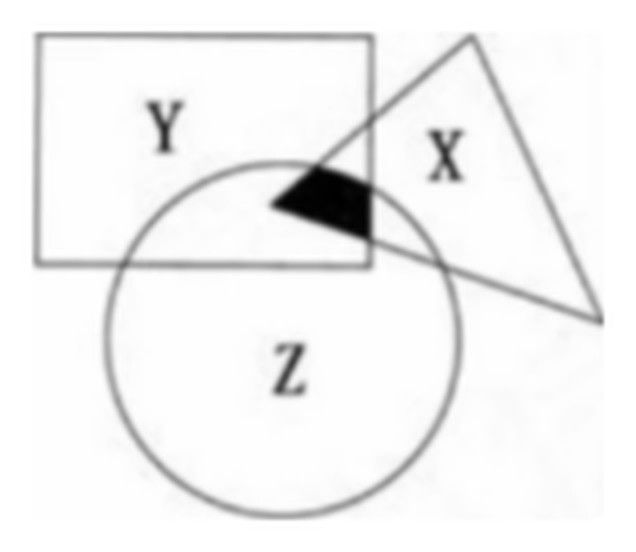
\includegraphics[width=0.20\textwidth]{figures/venn_XYZ_overlap.png}
\end{center}

\ifanswer
\solbegin
\step{设阴影部分的面积是 $x$，则 $290=64+180+160-24-70-36+x$，}
\step{$290=274+x$，$x=16$，故阴影部分的面积是 $16$.}
\solend

\fi

\item 如果集合 $A=\{1,2,3,\cdots,8\}$ 的子集 $B$ 满足：若 $2k\in B$，$k\in\N^{*}$，则 $2k+1\in B$，则称 $B$ 为 $A$ 的“好子集”，$A$ 的“好子集”有 \blankline[2.4em] 个.

\ifanswer
\solbegin
\step{由“好子集”定义得 $2$，$3$ 同时出现，$4$，$5$ 同时出现，$6$，$7$ 同时出现，}
\step{①当集合 $B$ 为空集时，满足题意；}
% 注：原卷此行印作「非空真子集共有 $2^4-1=15$ 种」，与同行算式冲突（$2^4-1=15$ 是**非空子集**数，
%     非空真子集应为 $2^4-2=14$），且与本段①（$B=\varnothing$）合起来恰构成「不含偶数的全体子集」，
%     故按文意订正为「非空子集」（段末总数 $1+15+24+12+2=54$ 不变）。
\step{②当集合 $B$ 中不存在偶数时，$\{1,3,5,7\}$ 的非空子集共有 $2^4-1=15$ 种；}
\step{③当集合 $B$ 中存在 $1$ 个偶数时，三个偶数中选择 $1$ 个，有 $C_3^1=3$ 种，}
\step{剩下 $3$ 个奇数不选，选 $1$ 个、$2$ 个、$3$ 个共有 $2^3=8$ 种，故共有 $24$ 种；}
\step{④当集合 $B$ 中存在 $2$ 个偶数时，三个偶数中选择 $2$ 个，有 $C_3^2=3$ 种，}
\step{剩下 $2$ 个奇数不选，选 $1$ 个、$2$ 个共有 $2^2=4$ 种，故共有 $12$ 种；}
\step{⑤当集合 $B$ 中存在 $3$ 个偶数时，三个偶数中选择 $3$ 个，有 $C_3^3=1$ 种，}
\step{剩下 $1$ 个奇数不选，选 $1$ 个共有 $2^1=2$ 种，故共有 $2$ 种；}
\step{所以 $A$ 的“好子集”共有 $1+15+24+12+2=54$ 种.}
\solend

\fi

\item 已知 $A=\{x\mid x=a^2-b^2,\ a\in\Z,b\in\Z,x\in\N^{*},x\leqslant 40\}$，则集合 $A$ 中共有 \blankline[2.4em] 个元素.

\ifanswer
\solbegin
\step{因为 $(k+1)^2-k^2=2k+1$，所以所有正奇数都属于集合 $A$，}
\step{又 $(2k+2)^2-(2k)^2=8k+4=4(2k+1)$，$(2k+1)^2-(2k-1)^2=8k=4\times 2k$，}
\step{因此所有 $4$ 的整数倍的正整数也属于 $A$，}
\step{若 $x=4k+2$，$k\in\N$，则 $a^2-b^2=(a+b)(a-b)=4k+2=2(2k+1)$，}
\step{则 $a+b$ 和 $a-b$ 中一定是一个取奇数，一个取偶数，}
\step{但是 $a,b\in\Z$ 时，$a+b$ 与 $a-b$ 同奇偶，所以此时无解，}
\step{即所有被 $4$ 除余 $2$ 的正整数都不属于 $A$，}
\step{所以每 $4$ 个数中，有 $3$ 个数属于集合 $A$，则集合 $A$ 中共含 $30$ 个元素.}
\solend

\fi

\item 十个元素组成的集合 $M=\{19,93,-1,0,25,-78,-94,1,17,-2\}$，$M$ 的所有非空子集记为 $M_i$（$i=1,2,\cdots,1023$），每一非空子集中所有元素的乘积记为 $m_i$（$i=1,2,\cdots,1023$），则 $m_1+m_2+\cdots+m_{1023}=$ \blankline[3em].

\ifanswer
\solbegin
\step{因为 $M$ 的所有非空子集为 $M_i$（$i=1,2,\cdots,1023$），这 $1023$ 个子集分成以下几种情况：}
\step{①含 $0$ 的子集有 $512$ 个，这些子集均满足 $m_i=0$；}
\step{②不含 $0$，含 $-1$ 且还含有其它元素的子集有 $255$ 个，}
\step{③不含 $0$，不含 $-1$ 但含有其它元素的子集有 $255$ 个，}
\step{④只含 $-1$ 的子集一个 $\{-1\}$，满足 $m_i=-1$；}
\step{其中②③中的集合是一一对应的，且满足 $m_i$ 对应成相反数，}
\step{故 $m_1+m_2+m_3+\cdots+m_{1023}=512\times 0+255\times 0-1=-1$.}
\solend

\fi

\item 已知 $M=\{(x,y)\mid |xy|=a\}$，$N=\{(x,y)\mid |xy|+1=|x|+|y|\}$，若集合 $M\cap N$ 中的点恰是正八边形的 $8$ 个顶点，则 $a=$ \blankline[2.4em].

\begin{center}
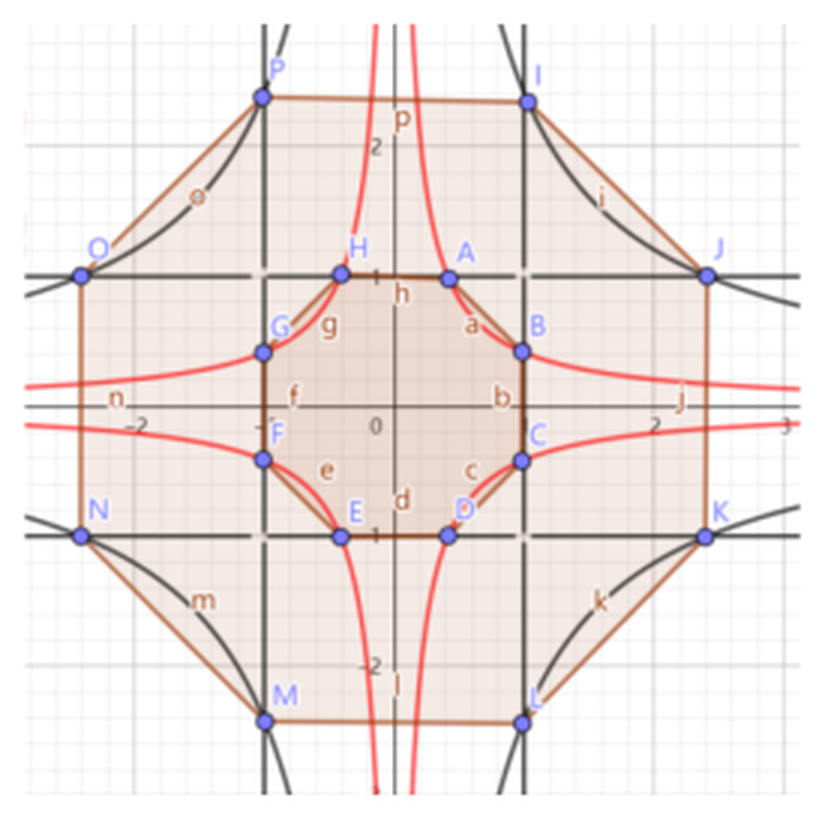
\includegraphics[width=0.44\textwidth]{figures/hyperbola_octagon.png}
\end{center}

\ifanswer
\solbegin
\step{$|xy|=a$ 和 $|xy|+1=|x|+|y|$ 的图像关于坐标轴均对称，只需考虑第一象限即可，}
\step{当 $x>0$，$y>0$ 时，$|xy|+1=|x|+|y|$ 即 $xy+1=x+y$，}
\step{即 $(x-1)(y-1)=0$，}
\step{即 $x=1$ 或 $y=1$，由对称性，作出完整的图像，}
\step{对于 $|xy|=a$，为四段双曲线，}
\step{考虑点 $A(I)(a,1)$，$B(J)(1,a)$，$C(K)(1,-a)$，}
\step{由 $AB=AC$ 得 $\sqrt{(a-1)^2+(1-a)^2}=2a$，解得 $a=\sqrt{2}\pm 1$.}
\solend

\fi

\item 集合 $A$ 是 $\{1,2,3,\cdots,100\}$ 的子集，若 $x\in A$，则 $2x\notin A$，$A$ 中的元素最多有 \blankline[2.4em] 个.

\ifanswer
\solbegin
\step{显然 $51$ 到 $100$ 共 $50$ 个可以，那么从 $1$ 到 $25$ 再 $2$ 倍不会超过 $50$，}
\step{$1$ 到 $25$ 中所有奇数都可以放到子集中，共有 $13$ 个，}
\step{再看偶数，$24=2\times 12$，$22=2\times 11$，$20=2\times 10$，$18=2\times 9$，$16=2\times 8$，}
% 注：末行照原卷抄录。原卷上一行列出 5 个偶数（24、22、20、18、16）而结论写「共有 $50+13+4=67$」，
%     此处的 $4$ 应作「另加 4 个元素」解（穷举验证集合 $A$ 的最大元素数确为 67），非笔误，故不改。
\step{及最后的 $4$，所以，共有 $50+13+4=67$.}
\solend

\fi

\end{enumerate}

\bigsec{二、选择题}

\begin{enumerate}
\setcounter{enumi}{13}

\item 下列各组集合中相等的是（\quad）.

①$P=\{x\mid x=2n,n\in\Z\}$，$Q=\{x\mid x=2(n-1),n\in\Z\}$；

②$P=\{x\mid x^2-1=0\}$，$Q=\left\{x\left|x=\dfrac{1+(-1)^n}{2},n\in\Z\right.\right\}$；

③$P=\{x\mid x=2m+1,m\in\Z\}$，$Q=\{x\mid x=4m\pm 1,m\in\Z\}$；

④$P=\{y\mid y=x^2+1\}$，$Q=\{x\mid y=x^2+1\}$.

\keepwithprev
A. ①②③④\qquad B. ①③\qquad C. ①②④\qquad D. ②④

\ans{B}

\item 如果一个命题的逆命题是真命题，那么这个命题的否命题是（\quad）

\keepwithprev
A. 真命题\qquad B. 假命题

C. 不一定是真命题\qquad D. 不一定是假命题

\ans{A}

\ifanswer
\solbegin
\step{一个命题的逆命题与这个命题的否命题是逆否命题，}
\step{它们的真假性相同，所以逆命题是真命题时，它们的否命题也是真命题. 故选 A.}
\solend

\fi

\item 设 $U$ 表示全集，下列命题中假命题有（\quad）

①若 $A\cap B=U$，则 $A=B=U$；②若 $A\cup B=\varnothing$，则 $A=B=\varnothing$；

③若 $A\cap B=\varnothing$，则 $\overline{A}\cup\overline{B}=U$；④若 $A\cup B=U$，则 $\overline{A}\cap\overline{B}=\varnothing$；

⑤若 $A\subseteq B$，则 $\overline{A}\supseteq\overline{B}$；⑥$\varnothing\in\{\varnothing\}$；⑦$\varnothing\subseteq\{\varnothing\}$.

\keepwithprev
A. $0$\qquad B. $1$\qquad C. $2$\qquad D. $3$

\ans{A}

\ifanswer
\solbegin
\step{全部正确，故选 A.}
\solend

\fi

\end{enumerate}

\bigsec{三、解答题}

\begin{enumerate}
\setcounter{enumi}{16}

\item 已知集合 $A=\{x\mid x^2-3x+2=0\}$，$B=\{x\mid x^2-bx+b-1=0\}$，$C=\{x\mid x^2-cx+2=0\}$.

\begin{enumerate}[label=(\arabic*)]
\item 若 $A\cup B=A$，求实数 $b$ 的值；
\item 若 $A\cap C=C$，求实数 $c$ 的取值范围.
\end{enumerate}

\ifanswer
\solbegin
\stepm{(1)}{$A=\{1,2\}$，$B=\{x\mid(x-1)(x-b+1)=0\}$，}
\step{由 $A\cup B=A$ 得 $b-1=1$ 或 $b-1=2$，所以 $b=2$ 或 $b=3$.}
\stepm{(2)}{由 $A\cap C=C$ 得 $C\subseteq A$，则 $C=\varnothing$ 或 $C=\{1\}$ 或 $C=\{2\}$ 或 $C=\{1,2\}$，}
\step{若 $C=\varnothing$，则 $\Delta=c^2-8<0$，解得 $-2\sqrt{2}<c<2\sqrt{2}$；}
\step{若 $C=\{1\}$，则 $\begin{cases}1+1=c\\ 1\times 1=2\end{cases}$，不可能；}
\step{若 $C=\{2\}$，则 $\begin{cases}2+2=c\\ 2\times 2=2\end{cases}$，不可能；}
\step{若 $C=\{1,2\}$，则 $\begin{cases}1+2=c\\ 1\times 2=2\end{cases}$，符合题意，$c=3$.}
\step{综上所述，$-2\sqrt{2}<c<2\sqrt{2}$ 或 $c=3$.}
\solend

\fi

\ansspace[6]

\item 已知全集 $U=\R$，$A=\{x\mid x^2+px+12=0\}$，$B=\{x\mid x^2-5x+q=0\}$，$\overline{A}\cap B=\{2\}$，求 $p+q$ 的值.

\ifanswer
\solbegin
\step{因为 $\overline{A}\cap B=\{2\}$，所以 $2\in B$，$2\notin A$，}
\step{所以 $2^2-5\times 2+q=0$，解得 $q=6$，$B=\{2,3\}$，}
\step{因为 $\overline{A}\cap B=\{2\}$，$B=\{2,3\}$，所以 $3\in A$，}
\step{所以 $3^2+p\times 3+12=0$，所以 $p=-7$，所以 $p+q=-1$.}
\solend

\fi

\ansspace[5]

\item 求证：方程 $x^2-abx+a+b=0$，$x^2-(a+b)x+ab=0$，其中 $a>2$，$b>2$ 没有公共根.

\ifanswer
\solbegin
\step{假设这两个方程有公共根 $\alpha$，则 $\alpha^2-ab\alpha+(a+b)=0$，$\alpha^2-(a+b)\alpha+ab=0$，}
\step{两式相减得 $(ab-a-b)(\alpha+1)=0$，}
\step{因为 $a>2$，$b>2$，所以 $a-1>1$，$b-1>1$，所以 $(a-1)(b-1)>1$，}
\step{所以 $ab-a-b>0$，所以 $\alpha+1=0$，所以 $\alpha=-1$，}
\step{代入第一个方程，得 $1+ab+a+b=0$，即 $(a+1)(b+1)=0$，}
\step{因为 $a>2$，$b>2$，所以该式不成立，所以这两个方程没有公共根.}
\solend

\fi

\ansspace[9]

% 压轴题：其后已无内容，故作答区全用可丢弃胶水（\ansspace*），并在题目前先量一下版面。
\ansneed{7cm}

\item 若集合 $A$ 具有以下性质：①$0\in A$，$1\in A$；②若 $x$、$y\in A$，则 $x-y\in A$，且 $x\neq 0$ 时，$\dfrac{1}{x}\in A$；则称集合 $A$ 是“好集”.

\begin{enumerate}[label=(\arabic*)]
\item 分别判断集合 $B=\{-1,0,1\}$，有理数集 $\Q$ 是否是“好集”，并说明理由；
\item 设集合 $A$ 是“好集”，求证：若 $x$、$y\in A$，则 $x+y\in A$；
\item 对任意的一个“好集” $A$，分别判断下面命题的真假，并说明理由.

命题 $p$：若 $x$、$y\in A$，则必有 $xy\in A$；

命题 $q$：若 $x$、$y\in A$，且 $x\neq 0$，则必有 $\dfrac{y}{x}\in A$.
\end{enumerate}

\ifanswer
\solbegin
\stepm{(1)}{集合 $B$ 不是“好集”. 理由是：假设集合 $B$ 是“好集”.}
\step{因为 $-1\in B$，$1\in B$，所以 $-1-1=-2\in B$. 这与 $-2\notin B$ 矛盾.}
\step{有理数集 $\Q$ 是“好集”. 因为 $0\in\Q$，$1\in\Q$，}
\step{对任意的 $x$、$y\in\Q$，有 $x-y\in\Q$，且 $x\neq 0$ 时，$\dfrac{1}{x}\in\Q$，}
\step{所以有理数集 $\Q$ 是“好集”.}
\stepm{(2)}{因为集合 $A$ 是“好集”，所以 $0\in A$.}
\step{若 $x$、$y\in A$，则 $0-y\in A$，即 $-y\in A$，所以 $x-(-y)\in A$，即 $x+y\in A$.}
\stepm{(3)}{命题 $p$、$q$ 均为真命题. 理由如下：}
\step{对任意一个“好集” $A$，任取 $x$、$y\in A$，}
\step{若 $x$、$y$ 中有 $0$ 或 $1$ 时，显然 $xy\in A$.}
\step{下设 $x$、$y$ 均不为 $0$，$1$. 由定义得 $x-1$，$\dfrac{1}{x-1}$，$\dfrac{1}{x}\in A$，}
\step{所以 $\dfrac{1}{x-1}-\dfrac{1}{x}\in A$，即 $\dfrac{1}{x(x-1)}\in A$，所以 $x(x-1)\in A$.}
\step{由（2）得 $x(x-1)+x\in A$，即 $x^2\in A$. 同理可得 $y^2\in A$.}
\step{若 $x+y=0$ 或 $x+y=1$，则 $x^2+y^2\in A$.}
\step{若 $x+y\neq 0$ 且 $x+y\neq 1$，则 $(x+y)^2\in A$，}
\step{所以 $2xy=(x+y)^2-x^2-y^2\in A$，所以 $\dfrac{1}{2xy}\in A$，}
\step{由（2）得 $\dfrac{1}{xy}=\dfrac{1}{2xy}+\dfrac{1}{2xy}\in A$，所以 $xy\in A$.}
\step{综上，$xy\in A$，即命题 $p$ 为真命题.}
\step{若 $x$、$y\in A$，且 $x\neq 0$，则 $\dfrac{1}{x}\in A$，}
\step{所以 $\dfrac{y}{x}=y\cdot\dfrac{1}{x}\in A$，即命题 $q$ 为真命题.}
\solend

\fi

\ansspace*[11]

\end{enumerate}

\end{document}
"
% 紧凑版：xelatex "\def\iscompact{1}% 高一14_华师大二附中_集合与逻辑单元练习.tex
%   —— 高一上数学「2026-2027 年华师大二附中高一上 集合与逻辑单元练习」（试卷版/答案版）
% 试卷版：xelatex 高一14_华师大二附中_集合与逻辑单元练习.tex
% 答案版：xelatex "\def\isanswer{1}\input{高一14_华师大二附中_集合与逻辑单元练习.tex}"
% 紧凑版：xelatex "\def\iscompact{1}\input{高一14_华师大二附中_集合与逻辑单元练习.tex}"
%
% 原始材料是微信公众号图文（「魔都数学加油站」），正文为 6 张 PNG 页（1080×1527）。
% 原文本身就是一份**讲评版**——题目下方直接印出【答案】或【解析】，选择题更是把答案
% 直接印在括注里（第 14 题）。试题文字、答案与解析均照原卷录入，未改内容。卷面上的
% 粉色斜水印「魔都数学加油站」属水印，未录入。
%
% 与原卷的排版差异（均已在 README「说明」中交代）：
%   ① 原文自**第 3 题**起（第 1、2 题未在该文中发布），故本稿题号亦自 3 起；
%   ② 原卷未印分节标题，本稿按题型补出「一、填空题」「二、选择题」「三、解答题」三节；
%   ③ 原卷填空、选择题的答案直接印在题目下方（第 14 题印在括注里），本稿统一改为
%      试卷版隐去、答案版以【答案】或【解析】给出，使两版彻底分离；
%   ④ 原卷的 $\R$、$\Q$、$\Z$、$\N$、$\N^{*}$ 时作正体 $R$、$Q$、$Z$、$N$、$N^*$，
%      本稿按全稿惯例统一写作 $\R$、$\Q$、$\Z$、$\N$、$\N^{*}$；
%   ⑤ 原卷中文括注用**半角**括号（第 4 题「(填“真”或“假”)」、第 15 题「是(  )」、
%      第 16 题「有(    )」，均已放大核实），本稿按全稿惯例排全角；
%   ⑥ 第 3 题题干作「$a$ 为**指定**实数」、同题解析作「$a$ 为**给定**的实数」，二者同义，
%      本稿两处均照原卷抄录（未统一）。

% 原卷笔误一处（已逐处放大到能看清字形后核对，本稿按文意订正，并在 README 中写明原委）：
%   ① 第 9 题【解析】② 原卷印「$\{1,3,5,7\}$ 的非空**真**子集共有 $2^4-1=15$ 种」，
%      与同行算式冲突（$2^4-1=15$ 是**非空子集**数，非空真子集应为 $2^4-2=14$），
%      且与本段①（$B=\varnothing$）合起来恰构成「不含偶数的全体子集」，故订正为「非空子集」，
%      段末总数 $1+15+24+12+2=54$ 不变。
%
% 原卷存疑一处（无法确证原意，本稿照抄并加 % 注）：
%   ① 第 12 题【解析】末行「由 $AB=AC$ 得 $\sqrt{(a-1)^2+(1-a)^2}=2a$，解得 $a=\sqrt2\pm1$」——
%      按此式只能解出 $a=\sqrt2-1$（$a=\sqrt2+1$ 处左端 $2$、右端 $4.83$，等式不成立），
%      而其答案 $a=\sqrt2\pm1$ 经数值验证是正确的（两值互为倒数，均使 $M\cap N$ 的 8 个交点按
%      $45^\circ$ 均布）。疑为解析此式笔误，但无法确证原意，本稿照抄原卷、未改。
%      同行上一行的「考虑点 $A(I)(a,1)$，$B(J)(1,a)$，$C(K)(1,-a)$」（点标 I/J/K 与
%      figures/hyperbola_octagon.png 中的标注一一对应）与本行等号右端的 $2a$，均照原卷录入；
%      2026-09-15 回原图逐处放大复核时发现曾误作 $A(1,a)$、$B(a,1)$、$C(-1,a)$ 与「$=2$」，
%      已按原卷订正（见 README「高一14—高一18 专记」）。

\documentclass[a4paper,11pt]{article}
\usepackage{common}

\begin{document}

\examtitlest[3]{2026--2027 年华师大二附中高一上}{集合与逻辑单元练习}

\bigsec{一、填空题}

\begin{enumerate}
\setcounter{enumi}{2}

\item 已知 $a$ 为指定实数，$M=\{x\mid x^2-3x-a^2+2=0\}$ 的非空真子集个数是 \blankline[2.4em].

\ifanswer
\solbegin
\step{集合 $M=\{x\mid x^2-3x-a^2+2=0\}$，$a$ 为给定的实数，}
\step{关于方程 $x^2-3x-a^2+2=0$，因为 $\Delta=(-3)^2-4(2-a^2)=4a^2+1>0$，}
\step{所以方程有两个不同的实根，所以 $M$ 中有两个元素，}
\step{所以集合 $M$ 的非空真子集的个数为 $2^2-2=2$.}
\solend

\fi

\item 判断下列命题的真假：（填“真”或“假”）

（1）任何集合都不是空集的子集 \blankline[2.4em]；

（2）一个有理数与一个无理数的和与积都是无理数 \blankline[2.4em]；

（3）如果一个整数 $n$ 的平方是偶数，那么 $n$ 是偶数 \blankline[2.4em].

\ans{假，假，真}

\item 请写出“如果两个三角形全等，那么它们的面积相等”的逆否命题：\blankline[3em].

\ifanswer
\solbegin
\step{如果两个三角形的面积不相等，则这两个三角形不全等.}
\solend

\fi

\item 已知 $U=\{(x,y)\mid x,y\in\R\}$，$M=\left\{(x,y)\left|\dfrac{y-2}{x-1}=3\right.\right\}$，$N=\{(x,y)\mid y=3x-1\}$，$\overline{M}\cap N=$ \blankline[3em].

\ans{$\{(1,2)\}$}

\item 已知集合 $A=\{x\mid 5x-a\leqslant 0\}$，$B=\{x\mid 6x-b>0\}$，$a$、$b\in\N$，且 $A\cap B\cap\N=\{2,3,4\}$，则整数对 $(a,b)$ 的个数为 \blankline[2.4em].

\ifanswer
\solbegin
\step{$A=\left\{x\left|x\leqslant\dfrac{a}{5}\right.\right\}$，$B=\left\{x\left|x>\dfrac{b}{6}\right.\right\}$，因为 $A\cap B\cap\N=\{2,3,4\}$，}
\step{所以 $4\leqslant\dfrac{a}{5}<5$，$1\leqslant\dfrac{b}{6}<2$，解得 $20\leqslant a<25$，$6\leqslant b<12$，}
\step{又 $a$、$b\in\N$，所以 $a=20$，$21$，$22$，$23$，$24$，$b=6$，$7$，$8$，$9$，$10$，$11$，}
\step{则整数对 $(a,b)$ 的个数为 $30$.}
\solend

\fi

\item 如图所示，$X$、$Y$、$Z$ 分别是面积为 $64$、$180$、$160$ 的三张不同形状的纸片，它们部分重叠放在一起盖在桌面上，总共盖住的面积为 $290$，且 $X$ 与 $Y$、$Y$ 与 $Z$、$Z$ 与 $X$ 重叠部分面积分别为 $24$、$70$、$36$，问阴影部分的面积是 \blankline[2.4em].

\begin{center}
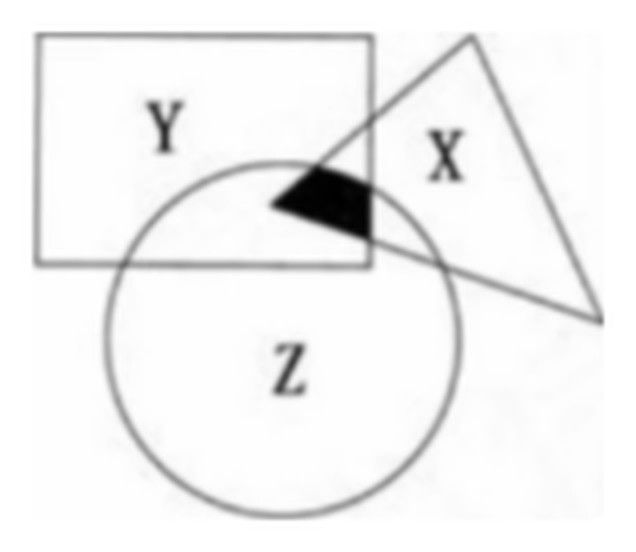
\includegraphics[width=0.20\textwidth]{figures/venn_XYZ_overlap.png}
\end{center}

\ifanswer
\solbegin
\step{设阴影部分的面积是 $x$，则 $290=64+180+160-24-70-36+x$，}
\step{$290=274+x$，$x=16$，故阴影部分的面积是 $16$.}
\solend

\fi

\item 如果集合 $A=\{1,2,3,\cdots,8\}$ 的子集 $B$ 满足：若 $2k\in B$，$k\in\N^{*}$，则 $2k+1\in B$，则称 $B$ 为 $A$ 的“好子集”，$A$ 的“好子集”有 \blankline[2.4em] 个.

\ifanswer
\solbegin
\step{由“好子集”定义得 $2$，$3$ 同时出现，$4$，$5$ 同时出现，$6$，$7$ 同时出现，}
\step{①当集合 $B$ 为空集时，满足题意；}
% 注：原卷此行印作「非空真子集共有 $2^4-1=15$ 种」，与同行算式冲突（$2^4-1=15$ 是**非空子集**数，
%     非空真子集应为 $2^4-2=14$），且与本段①（$B=\varnothing$）合起来恰构成「不含偶数的全体子集」，
%     故按文意订正为「非空子集」（段末总数 $1+15+24+12+2=54$ 不变）。
\step{②当集合 $B$ 中不存在偶数时，$\{1,3,5,7\}$ 的非空子集共有 $2^4-1=15$ 种；}
\step{③当集合 $B$ 中存在 $1$ 个偶数时，三个偶数中选择 $1$ 个，有 $C_3^1=3$ 种，}
\step{剩下 $3$ 个奇数不选，选 $1$ 个、$2$ 个、$3$ 个共有 $2^3=8$ 种，故共有 $24$ 种；}
\step{④当集合 $B$ 中存在 $2$ 个偶数时，三个偶数中选择 $2$ 个，有 $C_3^2=3$ 种，}
\step{剩下 $2$ 个奇数不选，选 $1$ 个、$2$ 个共有 $2^2=4$ 种，故共有 $12$ 种；}
\step{⑤当集合 $B$ 中存在 $3$ 个偶数时，三个偶数中选择 $3$ 个，有 $C_3^3=1$ 种，}
\step{剩下 $1$ 个奇数不选，选 $1$ 个共有 $2^1=2$ 种，故共有 $2$ 种；}
\step{所以 $A$ 的“好子集”共有 $1+15+24+12+2=54$ 种.}
\solend

\fi

\item 已知 $A=\{x\mid x=a^2-b^2,\ a\in\Z,b\in\Z,x\in\N^{*},x\leqslant 40\}$，则集合 $A$ 中共有 \blankline[2.4em] 个元素.

\ifanswer
\solbegin
\step{因为 $(k+1)^2-k^2=2k+1$，所以所有正奇数都属于集合 $A$，}
\step{又 $(2k+2)^2-(2k)^2=8k+4=4(2k+1)$，$(2k+1)^2-(2k-1)^2=8k=4\times 2k$，}
\step{因此所有 $4$ 的整数倍的正整数也属于 $A$，}
\step{若 $x=4k+2$，$k\in\N$，则 $a^2-b^2=(a+b)(a-b)=4k+2=2(2k+1)$，}
\step{则 $a+b$ 和 $a-b$ 中一定是一个取奇数，一个取偶数，}
\step{但是 $a,b\in\Z$ 时，$a+b$ 与 $a-b$ 同奇偶，所以此时无解，}
\step{即所有被 $4$ 除余 $2$ 的正整数都不属于 $A$，}
\step{所以每 $4$ 个数中，有 $3$ 个数属于集合 $A$，则集合 $A$ 中共含 $30$ 个元素.}
\solend

\fi

\item 十个元素组成的集合 $M=\{19,93,-1,0,25,-78,-94,1,17,-2\}$，$M$ 的所有非空子集记为 $M_i$（$i=1,2,\cdots,1023$），每一非空子集中所有元素的乘积记为 $m_i$（$i=1,2,\cdots,1023$），则 $m_1+m_2+\cdots+m_{1023}=$ \blankline[3em].

\ifanswer
\solbegin
\step{因为 $M$ 的所有非空子集为 $M_i$（$i=1,2,\cdots,1023$），这 $1023$ 个子集分成以下几种情况：}
\step{①含 $0$ 的子集有 $512$ 个，这些子集均满足 $m_i=0$；}
\step{②不含 $0$，含 $-1$ 且还含有其它元素的子集有 $255$ 个，}
\step{③不含 $0$，不含 $-1$ 但含有其它元素的子集有 $255$ 个，}
\step{④只含 $-1$ 的子集一个 $\{-1\}$，满足 $m_i=-1$；}
\step{其中②③中的集合是一一对应的，且满足 $m_i$ 对应成相反数，}
\step{故 $m_1+m_2+m_3+\cdots+m_{1023}=512\times 0+255\times 0-1=-1$.}
\solend

\fi

\item 已知 $M=\{(x,y)\mid |xy|=a\}$，$N=\{(x,y)\mid |xy|+1=|x|+|y|\}$，若集合 $M\cap N$ 中的点恰是正八边形的 $8$ 个顶点，则 $a=$ \blankline[2.4em].

\begin{center}
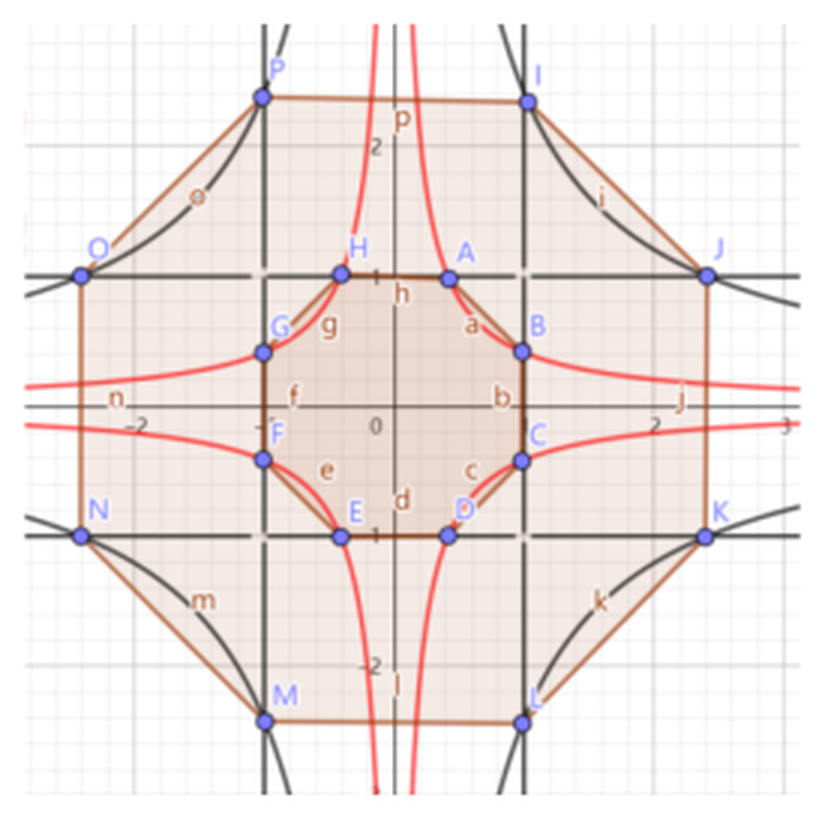
\includegraphics[width=0.44\textwidth]{figures/hyperbola_octagon.png}
\end{center}

\ifanswer
\solbegin
\step{$|xy|=a$ 和 $|xy|+1=|x|+|y|$ 的图像关于坐标轴均对称，只需考虑第一象限即可，}
\step{当 $x>0$，$y>0$ 时，$|xy|+1=|x|+|y|$ 即 $xy+1=x+y$，}
\step{即 $(x-1)(y-1)=0$，}
\step{即 $x=1$ 或 $y=1$，由对称性，作出完整的图像，}
\step{对于 $|xy|=a$，为四段双曲线，}
\step{考虑点 $A(I)(a,1)$，$B(J)(1,a)$，$C(K)(1,-a)$，}
\step{由 $AB=AC$ 得 $\sqrt{(a-1)^2+(1-a)^2}=2a$，解得 $a=\sqrt{2}\pm 1$.}
\solend

\fi

\item 集合 $A$ 是 $\{1,2,3,\cdots,100\}$ 的子集，若 $x\in A$，则 $2x\notin A$，$A$ 中的元素最多有 \blankline[2.4em] 个.

\ifanswer
\solbegin
\step{显然 $51$ 到 $100$ 共 $50$ 个可以，那么从 $1$ 到 $25$ 再 $2$ 倍不会超过 $50$，}
\step{$1$ 到 $25$ 中所有奇数都可以放到子集中，共有 $13$ 个，}
\step{再看偶数，$24=2\times 12$，$22=2\times 11$，$20=2\times 10$，$18=2\times 9$，$16=2\times 8$，}
% 注：末行照原卷抄录。原卷上一行列出 5 个偶数（24、22、20、18、16）而结论写「共有 $50+13+4=67$」，
%     此处的 $4$ 应作「另加 4 个元素」解（穷举验证集合 $A$ 的最大元素数确为 67），非笔误，故不改。
\step{及最后的 $4$，所以，共有 $50+13+4=67$.}
\solend

\fi

\end{enumerate}

\bigsec{二、选择题}

\begin{enumerate}
\setcounter{enumi}{13}

\item 下列各组集合中相等的是（\quad）.

①$P=\{x\mid x=2n,n\in\Z\}$，$Q=\{x\mid x=2(n-1),n\in\Z\}$；

②$P=\{x\mid x^2-1=0\}$，$Q=\left\{x\left|x=\dfrac{1+(-1)^n}{2},n\in\Z\right.\right\}$；

③$P=\{x\mid x=2m+1,m\in\Z\}$，$Q=\{x\mid x=4m\pm 1,m\in\Z\}$；

④$P=\{y\mid y=x^2+1\}$，$Q=\{x\mid y=x^2+1\}$.

\keepwithprev
A. ①②③④\qquad B. ①③\qquad C. ①②④\qquad D. ②④

\ans{B}

\item 如果一个命题的逆命题是真命题，那么这个命题的否命题是（\quad）

\keepwithprev
A. 真命题\qquad B. 假命题

C. 不一定是真命题\qquad D. 不一定是假命题

\ans{A}

\ifanswer
\solbegin
\step{一个命题的逆命题与这个命题的否命题是逆否命题，}
\step{它们的真假性相同，所以逆命题是真命题时，它们的否命题也是真命题. 故选 A.}
\solend

\fi

\item 设 $U$ 表示全集，下列命题中假命题有（\quad）

①若 $A\cap B=U$，则 $A=B=U$；②若 $A\cup B=\varnothing$，则 $A=B=\varnothing$；

③若 $A\cap B=\varnothing$，则 $\overline{A}\cup\overline{B}=U$；④若 $A\cup B=U$，则 $\overline{A}\cap\overline{B}=\varnothing$；

⑤若 $A\subseteq B$，则 $\overline{A}\supseteq\overline{B}$；⑥$\varnothing\in\{\varnothing\}$；⑦$\varnothing\subseteq\{\varnothing\}$.

\keepwithprev
A. $0$\qquad B. $1$\qquad C. $2$\qquad D. $3$

\ans{A}

\ifanswer
\solbegin
\step{全部正确，故选 A.}
\solend

\fi

\end{enumerate}

\bigsec{三、解答题}

\begin{enumerate}
\setcounter{enumi}{16}

\item 已知集合 $A=\{x\mid x^2-3x+2=0\}$，$B=\{x\mid x^2-bx+b-1=0\}$，$C=\{x\mid x^2-cx+2=0\}$.

\begin{enumerate}[label=(\arabic*)]
\item 若 $A\cup B=A$，求实数 $b$ 的值；
\item 若 $A\cap C=C$，求实数 $c$ 的取值范围.
\end{enumerate}

\ifanswer
\solbegin
\stepm{(1)}{$A=\{1,2\}$，$B=\{x\mid(x-1)(x-b+1)=0\}$，}
\step{由 $A\cup B=A$ 得 $b-1=1$ 或 $b-1=2$，所以 $b=2$ 或 $b=3$.}
\stepm{(2)}{由 $A\cap C=C$ 得 $C\subseteq A$，则 $C=\varnothing$ 或 $C=\{1\}$ 或 $C=\{2\}$ 或 $C=\{1,2\}$，}
\step{若 $C=\varnothing$，则 $\Delta=c^2-8<0$，解得 $-2\sqrt{2}<c<2\sqrt{2}$；}
\step{若 $C=\{1\}$，则 $\begin{cases}1+1=c\\ 1\times 1=2\end{cases}$，不可能；}
\step{若 $C=\{2\}$，则 $\begin{cases}2+2=c\\ 2\times 2=2\end{cases}$，不可能；}
\step{若 $C=\{1,2\}$，则 $\begin{cases}1+2=c\\ 1\times 2=2\end{cases}$，符合题意，$c=3$.}
\step{综上所述，$-2\sqrt{2}<c<2\sqrt{2}$ 或 $c=3$.}
\solend

\fi

\ansspace[6]

\item 已知全集 $U=\R$，$A=\{x\mid x^2+px+12=0\}$，$B=\{x\mid x^2-5x+q=0\}$，$\overline{A}\cap B=\{2\}$，求 $p+q$ 的值.

\ifanswer
\solbegin
\step{因为 $\overline{A}\cap B=\{2\}$，所以 $2\in B$，$2\notin A$，}
\step{所以 $2^2-5\times 2+q=0$，解得 $q=6$，$B=\{2,3\}$，}
\step{因为 $\overline{A}\cap B=\{2\}$，$B=\{2,3\}$，所以 $3\in A$，}
\step{所以 $3^2+p\times 3+12=0$，所以 $p=-7$，所以 $p+q=-1$.}
\solend

\fi

\ansspace[5]

\item 求证：方程 $x^2-abx+a+b=0$，$x^2-(a+b)x+ab=0$，其中 $a>2$，$b>2$ 没有公共根.

\ifanswer
\solbegin
\step{假设这两个方程有公共根 $\alpha$，则 $\alpha^2-ab\alpha+(a+b)=0$，$\alpha^2-(a+b)\alpha+ab=0$，}
\step{两式相减得 $(ab-a-b)(\alpha+1)=0$，}
\step{因为 $a>2$，$b>2$，所以 $a-1>1$，$b-1>1$，所以 $(a-1)(b-1)>1$，}
\step{所以 $ab-a-b>0$，所以 $\alpha+1=0$，所以 $\alpha=-1$，}
\step{代入第一个方程，得 $1+ab+a+b=0$，即 $(a+1)(b+1)=0$，}
\step{因为 $a>2$，$b>2$，所以该式不成立，所以这两个方程没有公共根.}
\solend

\fi

\ansspace[9]

% 压轴题：其后已无内容，故作答区全用可丢弃胶水（\ansspace*），并在题目前先量一下版面。
\ansneed{7cm}

\item 若集合 $A$ 具有以下性质：①$0\in A$，$1\in A$；②若 $x$、$y\in A$，则 $x-y\in A$，且 $x\neq 0$ 时，$\dfrac{1}{x}\in A$；则称集合 $A$ 是“好集”.

\begin{enumerate}[label=(\arabic*)]
\item 分别判断集合 $B=\{-1,0,1\}$，有理数集 $\Q$ 是否是“好集”，并说明理由；
\item 设集合 $A$ 是“好集”，求证：若 $x$、$y\in A$，则 $x+y\in A$；
\item 对任意的一个“好集” $A$，分别判断下面命题的真假，并说明理由.

命题 $p$：若 $x$、$y\in A$，则必有 $xy\in A$；

命题 $q$：若 $x$、$y\in A$，且 $x\neq 0$，则必有 $\dfrac{y}{x}\in A$.
\end{enumerate}

\ifanswer
\solbegin
\stepm{(1)}{集合 $B$ 不是“好集”. 理由是：假设集合 $B$ 是“好集”.}
\step{因为 $-1\in B$，$1\in B$，所以 $-1-1=-2\in B$. 这与 $-2\notin B$ 矛盾.}
\step{有理数集 $\Q$ 是“好集”. 因为 $0\in\Q$，$1\in\Q$，}
\step{对任意的 $x$、$y\in\Q$，有 $x-y\in\Q$，且 $x\neq 0$ 时，$\dfrac{1}{x}\in\Q$，}
\step{所以有理数集 $\Q$ 是“好集”.}
\stepm{(2)}{因为集合 $A$ 是“好集”，所以 $0\in A$.}
\step{若 $x$、$y\in A$，则 $0-y\in A$，即 $-y\in A$，所以 $x-(-y)\in A$，即 $x+y\in A$.}
\stepm{(3)}{命题 $p$、$q$ 均为真命题. 理由如下：}
\step{对任意一个“好集” $A$，任取 $x$、$y\in A$，}
\step{若 $x$、$y$ 中有 $0$ 或 $1$ 时，显然 $xy\in A$.}
\step{下设 $x$、$y$ 均不为 $0$，$1$. 由定义得 $x-1$，$\dfrac{1}{x-1}$，$\dfrac{1}{x}\in A$，}
\step{所以 $\dfrac{1}{x-1}-\dfrac{1}{x}\in A$，即 $\dfrac{1}{x(x-1)}\in A$，所以 $x(x-1)\in A$.}
\step{由（2）得 $x(x-1)+x\in A$，即 $x^2\in A$. 同理可得 $y^2\in A$.}
\step{若 $x+y=0$ 或 $x+y=1$，则 $x^2+y^2\in A$.}
\step{若 $x+y\neq 0$ 且 $x+y\neq 1$，则 $(x+y)^2\in A$，}
\step{所以 $2xy=(x+y)^2-x^2-y^2\in A$，所以 $\dfrac{1}{2xy}\in A$，}
\step{由（2）得 $\dfrac{1}{xy}=\dfrac{1}{2xy}+\dfrac{1}{2xy}\in A$，所以 $xy\in A$.}
\step{综上，$xy\in A$，即命题 $p$ 为真命题.}
\step{若 $x$、$y\in A$，且 $x\neq 0$，则 $\dfrac{1}{x}\in A$，}
\step{所以 $\dfrac{y}{x}=y\cdot\dfrac{1}{x}\in A$，即命题 $q$ 为真命题.}
\solend

\fi

\ansspace*[11]

\end{enumerate}

\end{document}
"
%
% 原始材料是微信公众号图文（「魔都数学加油站」），正文为 6 张 PNG 页（1080×1527）。
% 原文本身就是一份**讲评版**——题目下方直接印出【答案】或【解析】，选择题更是把答案
% 直接印在括注里（第 14 题）。试题文字、答案与解析均照原卷录入，未改内容。卷面上的
% 粉色斜水印「魔都数学加油站」属水印，未录入。
%
% 与原卷的排版差异（均已在 README「说明」中交代）：
%   ① 原文自**第 3 题**起（第 1、2 题未在该文中发布），故本稿题号亦自 3 起；
%   ② 原卷未印分节标题，本稿按题型补出「一、填空题」「二、选择题」「三、解答题」三节；
%   ③ 原卷填空、选择题的答案直接印在题目下方（第 14 题印在括注里），本稿统一改为
%      试卷版隐去、答案版以【答案】或【解析】给出，使两版彻底分离；
%   ④ 原卷的 $\R$、$\Q$、$\Z$、$\N$、$\N^{*}$ 时作正体 $R$、$Q$、$Z$、$N$、$N^*$，
%      本稿按全稿惯例统一写作 $\R$、$\Q$、$\Z$、$\N$、$\N^{*}$；
%   ⑤ 原卷中文括注用**半角**括号（第 4 题「(填“真”或“假”)」、第 15 题「是(  )」、
%      第 16 题「有(    )」，均已放大核实），本稿按全稿惯例排全角；
%   ⑥ 第 3 题题干作「$a$ 为**指定**实数」、同题解析作「$a$ 为**给定**的实数」，二者同义，
%      本稿两处均照原卷抄录（未统一）。

% 原卷笔误一处（已逐处放大到能看清字形后核对，本稿按文意订正，并在 README 中写明原委）：
%   ① 第 9 题【解析】② 原卷印「$\{1,3,5,7\}$ 的非空**真**子集共有 $2^4-1=15$ 种」，
%      与同行算式冲突（$2^4-1=15$ 是**非空子集**数，非空真子集应为 $2^4-2=14$），
%      且与本段①（$B=\varnothing$）合起来恰构成「不含偶数的全体子集」，故订正为「非空子集」，
%      段末总数 $1+15+24+12+2=54$ 不变。
%
% 原卷存疑一处（无法确证原意，本稿照抄并加 % 注）：
%   ① 第 12 题【解析】末行「由 $AB=AC$ 得 $\sqrt{(a-1)^2+(1-a)^2}=2a$，解得 $a=\sqrt2\pm1$」——
%      按此式只能解出 $a=\sqrt2-1$（$a=\sqrt2+1$ 处左端 $2$、右端 $4.83$，等式不成立），
%      而其答案 $a=\sqrt2\pm1$ 经数值验证是正确的（两值互为倒数，均使 $M\cap N$ 的 8 个交点按
%      $45^\circ$ 均布）。疑为解析此式笔误，但无法确证原意，本稿照抄原卷、未改。
%      同行上一行的「考虑点 $A(I)(a,1)$，$B(J)(1,a)$，$C(K)(1,-a)$」（点标 I/J/K 与
%      figures/hyperbola_octagon.png 中的标注一一对应）与本行等号右端的 $2a$，均照原卷录入；
%      2026-09-15 回原图逐处放大复核时发现曾误作 $A(1,a)$、$B(a,1)$、$C(-1,a)$ 与「$=2$」，
%      已按原卷订正（见 README「高一14—高一18 专记」）。

\documentclass[a4paper,11pt]{article}
\usepackage{common}

\begin{document}

\examtitlest[3]{2026--2027 年华师大二附中高一上}{集合与逻辑单元练习}

\bigsec{一、填空题}

\begin{enumerate}
\setcounter{enumi}{2}

\item 已知 $a$ 为指定实数，$M=\{x\mid x^2-3x-a^2+2=0\}$ 的非空真子集个数是 \blankline[2.4em].

\ifanswer
\solbegin
\step{集合 $M=\{x\mid x^2-3x-a^2+2=0\}$，$a$ 为给定的实数，}
\step{关于方程 $x^2-3x-a^2+2=0$，因为 $\Delta=(-3)^2-4(2-a^2)=4a^2+1>0$，}
\step{所以方程有两个不同的实根，所以 $M$ 中有两个元素，}
\step{所以集合 $M$ 的非空真子集的个数为 $2^2-2=2$.}
\solend

\fi

\item 判断下列命题的真假：（填“真”或“假”）

（1）任何集合都不是空集的子集 \blankline[2.4em]；

（2）一个有理数与一个无理数的和与积都是无理数 \blankline[2.4em]；

（3）如果一个整数 $n$ 的平方是偶数，那么 $n$ 是偶数 \blankline[2.4em].

\ans{假，假，真}

\item 请写出“如果两个三角形全等，那么它们的面积相等”的逆否命题：\blankline[3em].

\ifanswer
\solbegin
\step{如果两个三角形的面积不相等，则这两个三角形不全等.}
\solend

\fi

\item 已知 $U=\{(x,y)\mid x,y\in\R\}$，$M=\left\{(x,y)\left|\dfrac{y-2}{x-1}=3\right.\right\}$，$N=\{(x,y)\mid y=3x-1\}$，$\overline{M}\cap N=$ \blankline[3em].

\ans{$\{(1,2)\}$}

\item 已知集合 $A=\{x\mid 5x-a\leqslant 0\}$，$B=\{x\mid 6x-b>0\}$，$a$、$b\in\N$，且 $A\cap B\cap\N=\{2,3,4\}$，则整数对 $(a,b)$ 的个数为 \blankline[2.4em].

\ifanswer
\solbegin
\step{$A=\left\{x\left|x\leqslant\dfrac{a}{5}\right.\right\}$，$B=\left\{x\left|x>\dfrac{b}{6}\right.\right\}$，因为 $A\cap B\cap\N=\{2,3,4\}$，}
\step{所以 $4\leqslant\dfrac{a}{5}<5$，$1\leqslant\dfrac{b}{6}<2$，解得 $20\leqslant a<25$，$6\leqslant b<12$，}
\step{又 $a$、$b\in\N$，所以 $a=20$，$21$，$22$，$23$，$24$，$b=6$，$7$，$8$，$9$，$10$，$11$，}
\step{则整数对 $(a,b)$ 的个数为 $30$.}
\solend

\fi

\item 如图所示，$X$、$Y$、$Z$ 分别是面积为 $64$、$180$、$160$ 的三张不同形状的纸片，它们部分重叠放在一起盖在桌面上，总共盖住的面积为 $290$，且 $X$ 与 $Y$、$Y$ 与 $Z$、$Z$ 与 $X$ 重叠部分面积分别为 $24$、$70$、$36$，问阴影部分的面积是 \blankline[2.4em].

\begin{center}
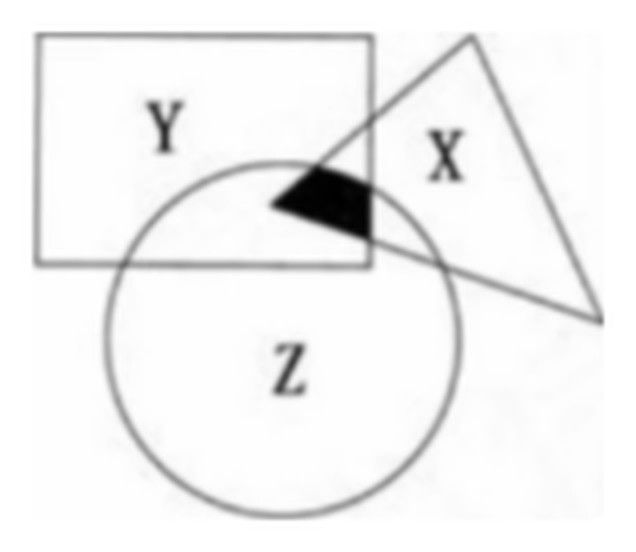
\includegraphics[width=0.20\textwidth]{figures/venn_XYZ_overlap.png}
\end{center}

\ifanswer
\solbegin
\step{设阴影部分的面积是 $x$，则 $290=64+180+160-24-70-36+x$，}
\step{$290=274+x$，$x=16$，故阴影部分的面积是 $16$.}
\solend

\fi

\item 如果集合 $A=\{1,2,3,\cdots,8\}$ 的子集 $B$ 满足：若 $2k\in B$，$k\in\N^{*}$，则 $2k+1\in B$，则称 $B$ 为 $A$ 的“好子集”，$A$ 的“好子集”有 \blankline[2.4em] 个.

\ifanswer
\solbegin
\step{由“好子集”定义得 $2$，$3$ 同时出现，$4$，$5$ 同时出现，$6$，$7$ 同时出现，}
\step{①当集合 $B$ 为空集时，满足题意；}
% 注：原卷此行印作「非空真子集共有 $2^4-1=15$ 种」，与同行算式冲突（$2^4-1=15$ 是**非空子集**数，
%     非空真子集应为 $2^4-2=14$），且与本段①（$B=\varnothing$）合起来恰构成「不含偶数的全体子集」，
%     故按文意订正为「非空子集」（段末总数 $1+15+24+12+2=54$ 不变）。
\step{②当集合 $B$ 中不存在偶数时，$\{1,3,5,7\}$ 的非空子集共有 $2^4-1=15$ 种；}
\step{③当集合 $B$ 中存在 $1$ 个偶数时，三个偶数中选择 $1$ 个，有 $C_3^1=3$ 种，}
\step{剩下 $3$ 个奇数不选，选 $1$ 个、$2$ 个、$3$ 个共有 $2^3=8$ 种，故共有 $24$ 种；}
\step{④当集合 $B$ 中存在 $2$ 个偶数时，三个偶数中选择 $2$ 个，有 $C_3^2=3$ 种，}
\step{剩下 $2$ 个奇数不选，选 $1$ 个、$2$ 个共有 $2^2=4$ 种，故共有 $12$ 种；}
\step{⑤当集合 $B$ 中存在 $3$ 个偶数时，三个偶数中选择 $3$ 个，有 $C_3^3=1$ 种，}
\step{剩下 $1$ 个奇数不选，选 $1$ 个共有 $2^1=2$ 种，故共有 $2$ 种；}
\step{所以 $A$ 的“好子集”共有 $1+15+24+12+2=54$ 种.}
\solend

\fi

\item 已知 $A=\{x\mid x=a^2-b^2,\ a\in\Z,b\in\Z,x\in\N^{*},x\leqslant 40\}$，则集合 $A$ 中共有 \blankline[2.4em] 个元素.

\ifanswer
\solbegin
\step{因为 $(k+1)^2-k^2=2k+1$，所以所有正奇数都属于集合 $A$，}
\step{又 $(2k+2)^2-(2k)^2=8k+4=4(2k+1)$，$(2k+1)^2-(2k-1)^2=8k=4\times 2k$，}
\step{因此所有 $4$ 的整数倍的正整数也属于 $A$，}
\step{若 $x=4k+2$，$k\in\N$，则 $a^2-b^2=(a+b)(a-b)=4k+2=2(2k+1)$，}
\step{则 $a+b$ 和 $a-b$ 中一定是一个取奇数，一个取偶数，}
\step{但是 $a,b\in\Z$ 时，$a+b$ 与 $a-b$ 同奇偶，所以此时无解，}
\step{即所有被 $4$ 除余 $2$ 的正整数都不属于 $A$，}
\step{所以每 $4$ 个数中，有 $3$ 个数属于集合 $A$，则集合 $A$ 中共含 $30$ 个元素.}
\solend

\fi

\item 十个元素组成的集合 $M=\{19,93,-1,0,25,-78,-94,1,17,-2\}$，$M$ 的所有非空子集记为 $M_i$（$i=1,2,\cdots,1023$），每一非空子集中所有元素的乘积记为 $m_i$（$i=1,2,\cdots,1023$），则 $m_1+m_2+\cdots+m_{1023}=$ \blankline[3em].

\ifanswer
\solbegin
\step{因为 $M$ 的所有非空子集为 $M_i$（$i=1,2,\cdots,1023$），这 $1023$ 个子集分成以下几种情况：}
\step{①含 $0$ 的子集有 $512$ 个，这些子集均满足 $m_i=0$；}
\step{②不含 $0$，含 $-1$ 且还含有其它元素的子集有 $255$ 个，}
\step{③不含 $0$，不含 $-1$ 但含有其它元素的子集有 $255$ 个，}
\step{④只含 $-1$ 的子集一个 $\{-1\}$，满足 $m_i=-1$；}
\step{其中②③中的集合是一一对应的，且满足 $m_i$ 对应成相反数，}
\step{故 $m_1+m_2+m_3+\cdots+m_{1023}=512\times 0+255\times 0-1=-1$.}
\solend

\fi

\item 已知 $M=\{(x,y)\mid |xy|=a\}$，$N=\{(x,y)\mid |xy|+1=|x|+|y|\}$，若集合 $M\cap N$ 中的点恰是正八边形的 $8$ 个顶点，则 $a=$ \blankline[2.4em].

\begin{center}
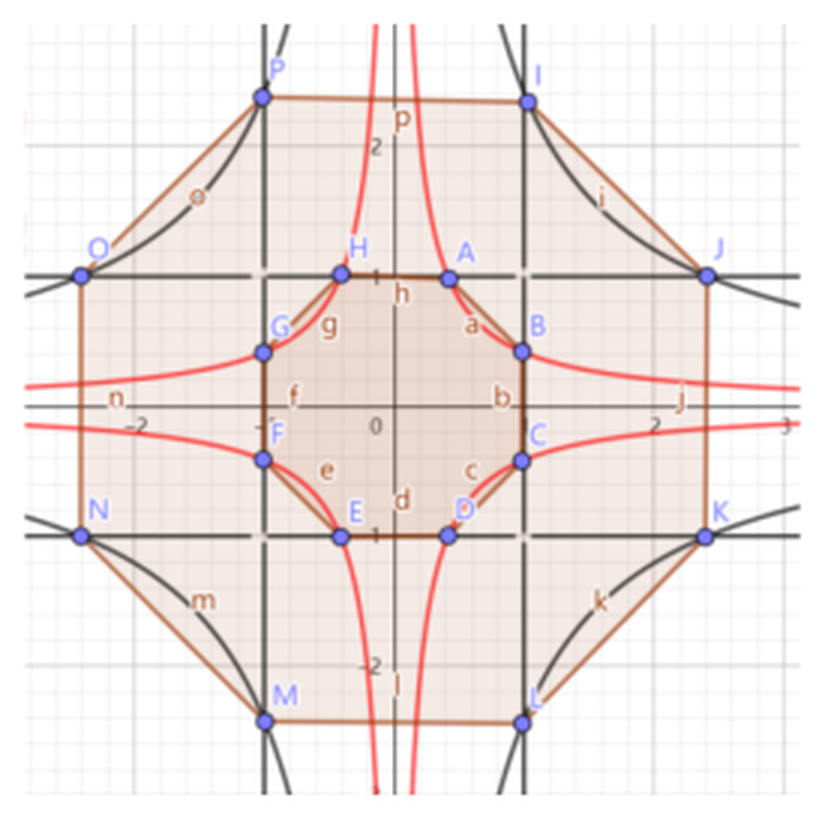
\includegraphics[width=0.44\textwidth]{figures/hyperbola_octagon.png}
\end{center}

\ifanswer
\solbegin
\step{$|xy|=a$ 和 $|xy|+1=|x|+|y|$ 的图像关于坐标轴均对称，只需考虑第一象限即可，}
\step{当 $x>0$，$y>0$ 时，$|xy|+1=|x|+|y|$ 即 $xy+1=x+y$，}
\step{即 $(x-1)(y-1)=0$，}
\step{即 $x=1$ 或 $y=1$，由对称性，作出完整的图像，}
\step{对于 $|xy|=a$，为四段双曲线，}
\step{考虑点 $A(I)(a,1)$，$B(J)(1,a)$，$C(K)(1,-a)$，}
\step{由 $AB=AC$ 得 $\sqrt{(a-1)^2+(1-a)^2}=2a$，解得 $a=\sqrt{2}\pm 1$.}
\solend

\fi

\item 集合 $A$ 是 $\{1,2,3,\cdots,100\}$ 的子集，若 $x\in A$，则 $2x\notin A$，$A$ 中的元素最多有 \blankline[2.4em] 个.

\ifanswer
\solbegin
\step{显然 $51$ 到 $100$ 共 $50$ 个可以，那么从 $1$ 到 $25$ 再 $2$ 倍不会超过 $50$，}
\step{$1$ 到 $25$ 中所有奇数都可以放到子集中，共有 $13$ 个，}
\step{再看偶数，$24=2\times 12$，$22=2\times 11$，$20=2\times 10$，$18=2\times 9$，$16=2\times 8$，}
% 注：末行照原卷抄录。原卷上一行列出 5 个偶数（24、22、20、18、16）而结论写「共有 $50+13+4=67$」，
%     此处的 $4$ 应作「另加 4 个元素」解（穷举验证集合 $A$ 的最大元素数确为 67），非笔误，故不改。
\step{及最后的 $4$，所以，共有 $50+13+4=67$.}
\solend

\fi

\end{enumerate}

\bigsec{二、选择题}

\begin{enumerate}
\setcounter{enumi}{13}

\item 下列各组集合中相等的是（\quad）.

①$P=\{x\mid x=2n,n\in\Z\}$，$Q=\{x\mid x=2(n-1),n\in\Z\}$；

②$P=\{x\mid x^2-1=0\}$，$Q=\left\{x\left|x=\dfrac{1+(-1)^n}{2},n\in\Z\right.\right\}$；

③$P=\{x\mid x=2m+1,m\in\Z\}$，$Q=\{x\mid x=4m\pm 1,m\in\Z\}$；

④$P=\{y\mid y=x^2+1\}$，$Q=\{x\mid y=x^2+1\}$.

\keepwithprev
A. ①②③④\qquad B. ①③\qquad C. ①②④\qquad D. ②④

\ans{B}

\item 如果一个命题的逆命题是真命题，那么这个命题的否命题是（\quad）

\keepwithprev
A. 真命题\qquad B. 假命题

C. 不一定是真命题\qquad D. 不一定是假命题

\ans{A}

\ifanswer
\solbegin
\step{一个命题的逆命题与这个命题的否命题是逆否命题，}
\step{它们的真假性相同，所以逆命题是真命题时，它们的否命题也是真命题. 故选 A.}
\solend

\fi

\item 设 $U$ 表示全集，下列命题中假命题有（\quad）

①若 $A\cap B=U$，则 $A=B=U$；②若 $A\cup B=\varnothing$，则 $A=B=\varnothing$；

③若 $A\cap B=\varnothing$，则 $\overline{A}\cup\overline{B}=U$；④若 $A\cup B=U$，则 $\overline{A}\cap\overline{B}=\varnothing$；

⑤若 $A\subseteq B$，则 $\overline{A}\supseteq\overline{B}$；⑥$\varnothing\in\{\varnothing\}$；⑦$\varnothing\subseteq\{\varnothing\}$.

\keepwithprev
A. $0$\qquad B. $1$\qquad C. $2$\qquad D. $3$

\ans{A}

\ifanswer
\solbegin
\step{全部正确，故选 A.}
\solend

\fi

\end{enumerate}

\bigsec{三、解答题}

\begin{enumerate}
\setcounter{enumi}{16}

\item 已知集合 $A=\{x\mid x^2-3x+2=0\}$，$B=\{x\mid x^2-bx+b-1=0\}$，$C=\{x\mid x^2-cx+2=0\}$.

\begin{enumerate}[label=(\arabic*)]
\item 若 $A\cup B=A$，求实数 $b$ 的值；
\item 若 $A\cap C=C$，求实数 $c$ 的取值范围.
\end{enumerate}

\ifanswer
\solbegin
\stepm{(1)}{$A=\{1,2\}$，$B=\{x\mid(x-1)(x-b+1)=0\}$，}
\step{由 $A\cup B=A$ 得 $b-1=1$ 或 $b-1=2$，所以 $b=2$ 或 $b=3$.}
\stepm{(2)}{由 $A\cap C=C$ 得 $C\subseteq A$，则 $C=\varnothing$ 或 $C=\{1\}$ 或 $C=\{2\}$ 或 $C=\{1,2\}$，}
\step{若 $C=\varnothing$，则 $\Delta=c^2-8<0$，解得 $-2\sqrt{2}<c<2\sqrt{2}$；}
\step{若 $C=\{1\}$，则 $\begin{cases}1+1=c\\ 1\times 1=2\end{cases}$，不可能；}
\step{若 $C=\{2\}$，则 $\begin{cases}2+2=c\\ 2\times 2=2\end{cases}$，不可能；}
\step{若 $C=\{1,2\}$，则 $\begin{cases}1+2=c\\ 1\times 2=2\end{cases}$，符合题意，$c=3$.}
\step{综上所述，$-2\sqrt{2}<c<2\sqrt{2}$ 或 $c=3$.}
\solend

\fi

\ansspace[6]

\item 已知全集 $U=\R$，$A=\{x\mid x^2+px+12=0\}$，$B=\{x\mid x^2-5x+q=0\}$，$\overline{A}\cap B=\{2\}$，求 $p+q$ 的值.

\ifanswer
\solbegin
\step{因为 $\overline{A}\cap B=\{2\}$，所以 $2\in B$，$2\notin A$，}
\step{所以 $2^2-5\times 2+q=0$，解得 $q=6$，$B=\{2,3\}$，}
\step{因为 $\overline{A}\cap B=\{2\}$，$B=\{2,3\}$，所以 $3\in A$，}
\step{所以 $3^2+p\times 3+12=0$，所以 $p=-7$，所以 $p+q=-1$.}
\solend

\fi

\ansspace[5]

\item 求证：方程 $x^2-abx+a+b=0$，$x^2-(a+b)x+ab=0$，其中 $a>2$，$b>2$ 没有公共根.

\ifanswer
\solbegin
\step{假设这两个方程有公共根 $\alpha$，则 $\alpha^2-ab\alpha+(a+b)=0$，$\alpha^2-(a+b)\alpha+ab=0$，}
\step{两式相减得 $(ab-a-b)(\alpha+1)=0$，}
\step{因为 $a>2$，$b>2$，所以 $a-1>1$，$b-1>1$，所以 $(a-1)(b-1)>1$，}
\step{所以 $ab-a-b>0$，所以 $\alpha+1=0$，所以 $\alpha=-1$，}
\step{代入第一个方程，得 $1+ab+a+b=0$，即 $(a+1)(b+1)=0$，}
\step{因为 $a>2$，$b>2$，所以该式不成立，所以这两个方程没有公共根.}
\solend

\fi

\ansspace[9]

% 压轴题：其后已无内容，故作答区全用可丢弃胶水（\ansspace*），并在题目前先量一下版面。
\ansneed{7cm}

\item 若集合 $A$ 具有以下性质：①$0\in A$，$1\in A$；②若 $x$、$y\in A$，则 $x-y\in A$，且 $x\neq 0$ 时，$\dfrac{1}{x}\in A$；则称集合 $A$ 是“好集”.

\begin{enumerate}[label=(\arabic*)]
\item 分别判断集合 $B=\{-1,0,1\}$，有理数集 $\Q$ 是否是“好集”，并说明理由；
\item 设集合 $A$ 是“好集”，求证：若 $x$、$y\in A$，则 $x+y\in A$；
\item 对任意的一个“好集” $A$，分别判断下面命题的真假，并说明理由.

命题 $p$：若 $x$、$y\in A$，则必有 $xy\in A$；

命题 $q$：若 $x$、$y\in A$，且 $x\neq 0$，则必有 $\dfrac{y}{x}\in A$.
\end{enumerate}

\ifanswer
\solbegin
\stepm{(1)}{集合 $B$ 不是“好集”. 理由是：假设集合 $B$ 是“好集”.}
\step{因为 $-1\in B$，$1\in B$，所以 $-1-1=-2\in B$. 这与 $-2\notin B$ 矛盾.}
\step{有理数集 $\Q$ 是“好集”. 因为 $0\in\Q$，$1\in\Q$，}
\step{对任意的 $x$、$y\in\Q$，有 $x-y\in\Q$，且 $x\neq 0$ 时，$\dfrac{1}{x}\in\Q$，}
\step{所以有理数集 $\Q$ 是“好集”.}
\stepm{(2)}{因为集合 $A$ 是“好集”，所以 $0\in A$.}
\step{若 $x$、$y\in A$，则 $0-y\in A$，即 $-y\in A$，所以 $x-(-y)\in A$，即 $x+y\in A$.}
\stepm{(3)}{命题 $p$、$q$ 均为真命题. 理由如下：}
\step{对任意一个“好集” $A$，任取 $x$、$y\in A$，}
\step{若 $x$、$y$ 中有 $0$ 或 $1$ 时，显然 $xy\in A$.}
\step{下设 $x$、$y$ 均不为 $0$，$1$. 由定义得 $x-1$，$\dfrac{1}{x-1}$，$\dfrac{1}{x}\in A$，}
\step{所以 $\dfrac{1}{x-1}-\dfrac{1}{x}\in A$，即 $\dfrac{1}{x(x-1)}\in A$，所以 $x(x-1)\in A$.}
\step{由（2）得 $x(x-1)+x\in A$，即 $x^2\in A$. 同理可得 $y^2\in A$.}
\step{若 $x+y=0$ 或 $x+y=1$，则 $x^2+y^2\in A$.}
\step{若 $x+y\neq 0$ 且 $x+y\neq 1$，则 $(x+y)^2\in A$，}
\step{所以 $2xy=(x+y)^2-x^2-y^2\in A$，所以 $\dfrac{1}{2xy}\in A$，}
\step{由（2）得 $\dfrac{1}{xy}=\dfrac{1}{2xy}+\dfrac{1}{2xy}\in A$，所以 $xy\in A$.}
\step{综上，$xy\in A$，即命题 $p$ 为真命题.}
\step{若 $x$、$y\in A$，且 $x\neq 0$，则 $\dfrac{1}{x}\in A$，}
\step{所以 $\dfrac{y}{x}=y\cdot\dfrac{1}{x}\in A$，即命题 $q$ 为真命题.}
\solend

\fi

\ansspace*[11]

\end{enumerate}

\end{document}
"
% 紧凑版：xelatex "\def\iscompact{1}% 高一14_华师大二附中_集合与逻辑单元练习.tex
%   —— 高一上数学「2026-2027 年华师大二附中高一上 集合与逻辑单元练习」（试卷版/答案版）
% 试卷版：xelatex 高一14_华师大二附中_集合与逻辑单元练习.tex
% 答案版：xelatex "\def\isanswer{1}% 高一14_华师大二附中_集合与逻辑单元练习.tex
%   —— 高一上数学「2026-2027 年华师大二附中高一上 集合与逻辑单元练习」（试卷版/答案版）
% 试卷版：xelatex 高一14_华师大二附中_集合与逻辑单元练习.tex
% 答案版：xelatex "\def\isanswer{1}\input{高一14_华师大二附中_集合与逻辑单元练习.tex}"
% 紧凑版：xelatex "\def\iscompact{1}\input{高一14_华师大二附中_集合与逻辑单元练习.tex}"
%
% 原始材料是微信公众号图文（「魔都数学加油站」），正文为 6 张 PNG 页（1080×1527）。
% 原文本身就是一份**讲评版**——题目下方直接印出【答案】或【解析】，选择题更是把答案
% 直接印在括注里（第 14 题）。试题文字、答案与解析均照原卷录入，未改内容。卷面上的
% 粉色斜水印「魔都数学加油站」属水印，未录入。
%
% 与原卷的排版差异（均已在 README「说明」中交代）：
%   ① 原文自**第 3 题**起（第 1、2 题未在该文中发布），故本稿题号亦自 3 起；
%   ② 原卷未印分节标题，本稿按题型补出「一、填空题」「二、选择题」「三、解答题」三节；
%   ③ 原卷填空、选择题的答案直接印在题目下方（第 14 题印在括注里），本稿统一改为
%      试卷版隐去、答案版以【答案】或【解析】给出，使两版彻底分离；
%   ④ 原卷的 $\R$、$\Q$、$\Z$、$\N$、$\N^{*}$ 时作正体 $R$、$Q$、$Z$、$N$、$N^*$，
%      本稿按全稿惯例统一写作 $\R$、$\Q$、$\Z$、$\N$、$\N^{*}$；
%   ⑤ 原卷中文括注用**半角**括号（第 4 题「(填“真”或“假”)」、第 15 题「是(  )」、
%      第 16 题「有(    )」，均已放大核实），本稿按全稿惯例排全角；
%   ⑥ 第 3 题题干作「$a$ 为**指定**实数」、同题解析作「$a$ 为**给定**的实数」，二者同义，
%      本稿两处均照原卷抄录（未统一）。

% 原卷笔误一处（已逐处放大到能看清字形后核对，本稿按文意订正，并在 README 中写明原委）：
%   ① 第 9 题【解析】② 原卷印「$\{1,3,5,7\}$ 的非空**真**子集共有 $2^4-1=15$ 种」，
%      与同行算式冲突（$2^4-1=15$ 是**非空子集**数，非空真子集应为 $2^4-2=14$），
%      且与本段①（$B=\varnothing$）合起来恰构成「不含偶数的全体子集」，故订正为「非空子集」，
%      段末总数 $1+15+24+12+2=54$ 不变。
%
% 原卷存疑一处（无法确证原意，本稿照抄并加 % 注）：
%   ① 第 12 题【解析】末行「由 $AB=AC$ 得 $\sqrt{(a-1)^2+(1-a)^2}=2a$，解得 $a=\sqrt2\pm1$」——
%      按此式只能解出 $a=\sqrt2-1$（$a=\sqrt2+1$ 处左端 $2$、右端 $4.83$，等式不成立），
%      而其答案 $a=\sqrt2\pm1$ 经数值验证是正确的（两值互为倒数，均使 $M\cap N$ 的 8 个交点按
%      $45^\circ$ 均布）。疑为解析此式笔误，但无法确证原意，本稿照抄原卷、未改。
%      同行上一行的「考虑点 $A(I)(a,1)$，$B(J)(1,a)$，$C(K)(1,-a)$」（点标 I/J/K 与
%      figures/hyperbola_octagon.png 中的标注一一对应）与本行等号右端的 $2a$，均照原卷录入；
%      2026-09-15 回原图逐处放大复核时发现曾误作 $A(1,a)$、$B(a,1)$、$C(-1,a)$ 与「$=2$」，
%      已按原卷订正（见 README「高一14—高一18 专记」）。

\documentclass[a4paper,11pt]{article}
\usepackage{common}

\begin{document}

\examtitlest[3]{2026--2027 年华师大二附中高一上}{集合与逻辑单元练习}

\bigsec{一、填空题}

\begin{enumerate}
\setcounter{enumi}{2}

\item 已知 $a$ 为指定实数，$M=\{x\mid x^2-3x-a^2+2=0\}$ 的非空真子集个数是 \blankline[2.4em].

\ifanswer
\solbegin
\step{集合 $M=\{x\mid x^2-3x-a^2+2=0\}$，$a$ 为给定的实数，}
\step{关于方程 $x^2-3x-a^2+2=0$，因为 $\Delta=(-3)^2-4(2-a^2)=4a^2+1>0$，}
\step{所以方程有两个不同的实根，所以 $M$ 中有两个元素，}
\step{所以集合 $M$ 的非空真子集的个数为 $2^2-2=2$.}
\solend

\fi

\item 判断下列命题的真假：（填“真”或“假”）

（1）任何集合都不是空集的子集 \blankline[2.4em]；

（2）一个有理数与一个无理数的和与积都是无理数 \blankline[2.4em]；

（3）如果一个整数 $n$ 的平方是偶数，那么 $n$ 是偶数 \blankline[2.4em].

\ans{假，假，真}

\item 请写出“如果两个三角形全等，那么它们的面积相等”的逆否命题：\blankline[3em].

\ifanswer
\solbegin
\step{如果两个三角形的面积不相等，则这两个三角形不全等.}
\solend

\fi

\item 已知 $U=\{(x,y)\mid x,y\in\R\}$，$M=\left\{(x,y)\left|\dfrac{y-2}{x-1}=3\right.\right\}$，$N=\{(x,y)\mid y=3x-1\}$，$\overline{M}\cap N=$ \blankline[3em].

\ans{$\{(1,2)\}$}

\item 已知集合 $A=\{x\mid 5x-a\leqslant 0\}$，$B=\{x\mid 6x-b>0\}$，$a$、$b\in\N$，且 $A\cap B\cap\N=\{2,3,4\}$，则整数对 $(a,b)$ 的个数为 \blankline[2.4em].

\ifanswer
\solbegin
\step{$A=\left\{x\left|x\leqslant\dfrac{a}{5}\right.\right\}$，$B=\left\{x\left|x>\dfrac{b}{6}\right.\right\}$，因为 $A\cap B\cap\N=\{2,3,4\}$，}
\step{所以 $4\leqslant\dfrac{a}{5}<5$，$1\leqslant\dfrac{b}{6}<2$，解得 $20\leqslant a<25$，$6\leqslant b<12$，}
\step{又 $a$、$b\in\N$，所以 $a=20$，$21$，$22$，$23$，$24$，$b=6$，$7$，$8$，$9$，$10$，$11$，}
\step{则整数对 $(a,b)$ 的个数为 $30$.}
\solend

\fi

\item 如图所示，$X$、$Y$、$Z$ 分别是面积为 $64$、$180$、$160$ 的三张不同形状的纸片，它们部分重叠放在一起盖在桌面上，总共盖住的面积为 $290$，且 $X$ 与 $Y$、$Y$ 与 $Z$、$Z$ 与 $X$ 重叠部分面积分别为 $24$、$70$、$36$，问阴影部分的面积是 \blankline[2.4em].

\begin{center}
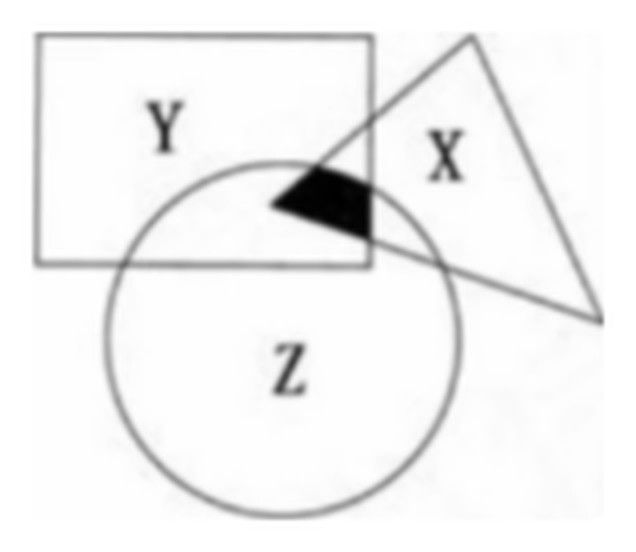
\includegraphics[width=0.20\textwidth]{figures/venn_XYZ_overlap.png}
\end{center}

\ifanswer
\solbegin
\step{设阴影部分的面积是 $x$，则 $290=64+180+160-24-70-36+x$，}
\step{$290=274+x$，$x=16$，故阴影部分的面积是 $16$.}
\solend

\fi

\item 如果集合 $A=\{1,2,3,\cdots,8\}$ 的子集 $B$ 满足：若 $2k\in B$，$k\in\N^{*}$，则 $2k+1\in B$，则称 $B$ 为 $A$ 的“好子集”，$A$ 的“好子集”有 \blankline[2.4em] 个.

\ifanswer
\solbegin
\step{由“好子集”定义得 $2$，$3$ 同时出现，$4$，$5$ 同时出现，$6$，$7$ 同时出现，}
\step{①当集合 $B$ 为空集时，满足题意；}
% 注：原卷此行印作「非空真子集共有 $2^4-1=15$ 种」，与同行算式冲突（$2^4-1=15$ 是**非空子集**数，
%     非空真子集应为 $2^4-2=14$），且与本段①（$B=\varnothing$）合起来恰构成「不含偶数的全体子集」，
%     故按文意订正为「非空子集」（段末总数 $1+15+24+12+2=54$ 不变）。
\step{②当集合 $B$ 中不存在偶数时，$\{1,3,5,7\}$ 的非空子集共有 $2^4-1=15$ 种；}
\step{③当集合 $B$ 中存在 $1$ 个偶数时，三个偶数中选择 $1$ 个，有 $C_3^1=3$ 种，}
\step{剩下 $3$ 个奇数不选，选 $1$ 个、$2$ 个、$3$ 个共有 $2^3=8$ 种，故共有 $24$ 种；}
\step{④当集合 $B$ 中存在 $2$ 个偶数时，三个偶数中选择 $2$ 个，有 $C_3^2=3$ 种，}
\step{剩下 $2$ 个奇数不选，选 $1$ 个、$2$ 个共有 $2^2=4$ 种，故共有 $12$ 种；}
\step{⑤当集合 $B$ 中存在 $3$ 个偶数时，三个偶数中选择 $3$ 个，有 $C_3^3=1$ 种，}
\step{剩下 $1$ 个奇数不选，选 $1$ 个共有 $2^1=2$ 种，故共有 $2$ 种；}
\step{所以 $A$ 的“好子集”共有 $1+15+24+12+2=54$ 种.}
\solend

\fi

\item 已知 $A=\{x\mid x=a^2-b^2,\ a\in\Z,b\in\Z,x\in\N^{*},x\leqslant 40\}$，则集合 $A$ 中共有 \blankline[2.4em] 个元素.

\ifanswer
\solbegin
\step{因为 $(k+1)^2-k^2=2k+1$，所以所有正奇数都属于集合 $A$，}
\step{又 $(2k+2)^2-(2k)^2=8k+4=4(2k+1)$，$(2k+1)^2-(2k-1)^2=8k=4\times 2k$，}
\step{因此所有 $4$ 的整数倍的正整数也属于 $A$，}
\step{若 $x=4k+2$，$k\in\N$，则 $a^2-b^2=(a+b)(a-b)=4k+2=2(2k+1)$，}
\step{则 $a+b$ 和 $a-b$ 中一定是一个取奇数，一个取偶数，}
\step{但是 $a,b\in\Z$ 时，$a+b$ 与 $a-b$ 同奇偶，所以此时无解，}
\step{即所有被 $4$ 除余 $2$ 的正整数都不属于 $A$，}
\step{所以每 $4$ 个数中，有 $3$ 个数属于集合 $A$，则集合 $A$ 中共含 $30$ 个元素.}
\solend

\fi

\item 十个元素组成的集合 $M=\{19,93,-1,0,25,-78,-94,1,17,-2\}$，$M$ 的所有非空子集记为 $M_i$（$i=1,2,\cdots,1023$），每一非空子集中所有元素的乘积记为 $m_i$（$i=1,2,\cdots,1023$），则 $m_1+m_2+\cdots+m_{1023}=$ \blankline[3em].

\ifanswer
\solbegin
\step{因为 $M$ 的所有非空子集为 $M_i$（$i=1,2,\cdots,1023$），这 $1023$ 个子集分成以下几种情况：}
\step{①含 $0$ 的子集有 $512$ 个，这些子集均满足 $m_i=0$；}
\step{②不含 $0$，含 $-1$ 且还含有其它元素的子集有 $255$ 个，}
\step{③不含 $0$，不含 $-1$ 但含有其它元素的子集有 $255$ 个，}
\step{④只含 $-1$ 的子集一个 $\{-1\}$，满足 $m_i=-1$；}
\step{其中②③中的集合是一一对应的，且满足 $m_i$ 对应成相反数，}
\step{故 $m_1+m_2+m_3+\cdots+m_{1023}=512\times 0+255\times 0-1=-1$.}
\solend

\fi

\item 已知 $M=\{(x,y)\mid |xy|=a\}$，$N=\{(x,y)\mid |xy|+1=|x|+|y|\}$，若集合 $M\cap N$ 中的点恰是正八边形的 $8$ 个顶点，则 $a=$ \blankline[2.4em].

\begin{center}
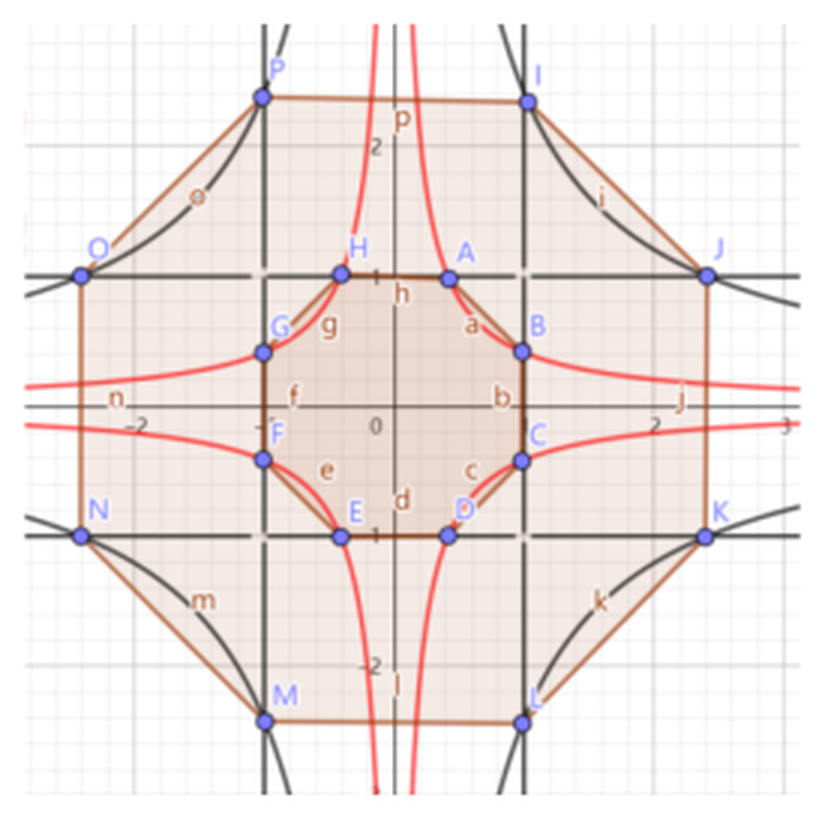
\includegraphics[width=0.44\textwidth]{figures/hyperbola_octagon.png}
\end{center}

\ifanswer
\solbegin
\step{$|xy|=a$ 和 $|xy|+1=|x|+|y|$ 的图像关于坐标轴均对称，只需考虑第一象限即可，}
\step{当 $x>0$，$y>0$ 时，$|xy|+1=|x|+|y|$ 即 $xy+1=x+y$，}
\step{即 $(x-1)(y-1)=0$，}
\step{即 $x=1$ 或 $y=1$，由对称性，作出完整的图像，}
\step{对于 $|xy|=a$，为四段双曲线，}
\step{考虑点 $A(I)(a,1)$，$B(J)(1,a)$，$C(K)(1,-a)$，}
\step{由 $AB=AC$ 得 $\sqrt{(a-1)^2+(1-a)^2}=2a$，解得 $a=\sqrt{2}\pm 1$.}
\solend

\fi

\item 集合 $A$ 是 $\{1,2,3,\cdots,100\}$ 的子集，若 $x\in A$，则 $2x\notin A$，$A$ 中的元素最多有 \blankline[2.4em] 个.

\ifanswer
\solbegin
\step{显然 $51$ 到 $100$ 共 $50$ 个可以，那么从 $1$ 到 $25$ 再 $2$ 倍不会超过 $50$，}
\step{$1$ 到 $25$ 中所有奇数都可以放到子集中，共有 $13$ 个，}
\step{再看偶数，$24=2\times 12$，$22=2\times 11$，$20=2\times 10$，$18=2\times 9$，$16=2\times 8$，}
% 注：末行照原卷抄录。原卷上一行列出 5 个偶数（24、22、20、18、16）而结论写「共有 $50+13+4=67$」，
%     此处的 $4$ 应作「另加 4 个元素」解（穷举验证集合 $A$ 的最大元素数确为 67），非笔误，故不改。
\step{及最后的 $4$，所以，共有 $50+13+4=67$.}
\solend

\fi

\end{enumerate}

\bigsec{二、选择题}

\begin{enumerate}
\setcounter{enumi}{13}

\item 下列各组集合中相等的是（\quad）.

①$P=\{x\mid x=2n,n\in\Z\}$，$Q=\{x\mid x=2(n-1),n\in\Z\}$；

②$P=\{x\mid x^2-1=0\}$，$Q=\left\{x\left|x=\dfrac{1+(-1)^n}{2},n\in\Z\right.\right\}$；

③$P=\{x\mid x=2m+1,m\in\Z\}$，$Q=\{x\mid x=4m\pm 1,m\in\Z\}$；

④$P=\{y\mid y=x^2+1\}$，$Q=\{x\mid y=x^2+1\}$.

\keepwithprev
A. ①②③④\qquad B. ①③\qquad C. ①②④\qquad D. ②④

\ans{B}

\item 如果一个命题的逆命题是真命题，那么这个命题的否命题是（\quad）

\keepwithprev
A. 真命题\qquad B. 假命题

C. 不一定是真命题\qquad D. 不一定是假命题

\ans{A}

\ifanswer
\solbegin
\step{一个命题的逆命题与这个命题的否命题是逆否命题，}
\step{它们的真假性相同，所以逆命题是真命题时，它们的否命题也是真命题. 故选 A.}
\solend

\fi

\item 设 $U$ 表示全集，下列命题中假命题有（\quad）

①若 $A\cap B=U$，则 $A=B=U$；②若 $A\cup B=\varnothing$，则 $A=B=\varnothing$；

③若 $A\cap B=\varnothing$，则 $\overline{A}\cup\overline{B}=U$；④若 $A\cup B=U$，则 $\overline{A}\cap\overline{B}=\varnothing$；

⑤若 $A\subseteq B$，则 $\overline{A}\supseteq\overline{B}$；⑥$\varnothing\in\{\varnothing\}$；⑦$\varnothing\subseteq\{\varnothing\}$.

\keepwithprev
A. $0$\qquad B. $1$\qquad C. $2$\qquad D. $3$

\ans{A}

\ifanswer
\solbegin
\step{全部正确，故选 A.}
\solend

\fi

\end{enumerate}

\bigsec{三、解答题}

\begin{enumerate}
\setcounter{enumi}{16}

\item 已知集合 $A=\{x\mid x^2-3x+2=0\}$，$B=\{x\mid x^2-bx+b-1=0\}$，$C=\{x\mid x^2-cx+2=0\}$.

\begin{enumerate}[label=(\arabic*)]
\item 若 $A\cup B=A$，求实数 $b$ 的值；
\item 若 $A\cap C=C$，求实数 $c$ 的取值范围.
\end{enumerate}

\ifanswer
\solbegin
\stepm{(1)}{$A=\{1,2\}$，$B=\{x\mid(x-1)(x-b+1)=0\}$，}
\step{由 $A\cup B=A$ 得 $b-1=1$ 或 $b-1=2$，所以 $b=2$ 或 $b=3$.}
\stepm{(2)}{由 $A\cap C=C$ 得 $C\subseteq A$，则 $C=\varnothing$ 或 $C=\{1\}$ 或 $C=\{2\}$ 或 $C=\{1,2\}$，}
\step{若 $C=\varnothing$，则 $\Delta=c^2-8<0$，解得 $-2\sqrt{2}<c<2\sqrt{2}$；}
\step{若 $C=\{1\}$，则 $\begin{cases}1+1=c\\ 1\times 1=2\end{cases}$，不可能；}
\step{若 $C=\{2\}$，则 $\begin{cases}2+2=c\\ 2\times 2=2\end{cases}$，不可能；}
\step{若 $C=\{1,2\}$，则 $\begin{cases}1+2=c\\ 1\times 2=2\end{cases}$，符合题意，$c=3$.}
\step{综上所述，$-2\sqrt{2}<c<2\sqrt{2}$ 或 $c=3$.}
\solend

\fi

\ansspace[6]

\item 已知全集 $U=\R$，$A=\{x\mid x^2+px+12=0\}$，$B=\{x\mid x^2-5x+q=0\}$，$\overline{A}\cap B=\{2\}$，求 $p+q$ 的值.

\ifanswer
\solbegin
\step{因为 $\overline{A}\cap B=\{2\}$，所以 $2\in B$，$2\notin A$，}
\step{所以 $2^2-5\times 2+q=0$，解得 $q=6$，$B=\{2,3\}$，}
\step{因为 $\overline{A}\cap B=\{2\}$，$B=\{2,3\}$，所以 $3\in A$，}
\step{所以 $3^2+p\times 3+12=0$，所以 $p=-7$，所以 $p+q=-1$.}
\solend

\fi

\ansspace[5]

\item 求证：方程 $x^2-abx+a+b=0$，$x^2-(a+b)x+ab=0$，其中 $a>2$，$b>2$ 没有公共根.

\ifanswer
\solbegin
\step{假设这两个方程有公共根 $\alpha$，则 $\alpha^2-ab\alpha+(a+b)=0$，$\alpha^2-(a+b)\alpha+ab=0$，}
\step{两式相减得 $(ab-a-b)(\alpha+1)=0$，}
\step{因为 $a>2$，$b>2$，所以 $a-1>1$，$b-1>1$，所以 $(a-1)(b-1)>1$，}
\step{所以 $ab-a-b>0$，所以 $\alpha+1=0$，所以 $\alpha=-1$，}
\step{代入第一个方程，得 $1+ab+a+b=0$，即 $(a+1)(b+1)=0$，}
\step{因为 $a>2$，$b>2$，所以该式不成立，所以这两个方程没有公共根.}
\solend

\fi

\ansspace[9]

% 压轴题：其后已无内容，故作答区全用可丢弃胶水（\ansspace*），并在题目前先量一下版面。
\ansneed{7cm}

\item 若集合 $A$ 具有以下性质：①$0\in A$，$1\in A$；②若 $x$、$y\in A$，则 $x-y\in A$，且 $x\neq 0$ 时，$\dfrac{1}{x}\in A$；则称集合 $A$ 是“好集”.

\begin{enumerate}[label=(\arabic*)]
\item 分别判断集合 $B=\{-1,0,1\}$，有理数集 $\Q$ 是否是“好集”，并说明理由；
\item 设集合 $A$ 是“好集”，求证：若 $x$、$y\in A$，则 $x+y\in A$；
\item 对任意的一个“好集” $A$，分别判断下面命题的真假，并说明理由.

命题 $p$：若 $x$、$y\in A$，则必有 $xy\in A$；

命题 $q$：若 $x$、$y\in A$，且 $x\neq 0$，则必有 $\dfrac{y}{x}\in A$.
\end{enumerate}

\ifanswer
\solbegin
\stepm{(1)}{集合 $B$ 不是“好集”. 理由是：假设集合 $B$ 是“好集”.}
\step{因为 $-1\in B$，$1\in B$，所以 $-1-1=-2\in B$. 这与 $-2\notin B$ 矛盾.}
\step{有理数集 $\Q$ 是“好集”. 因为 $0\in\Q$，$1\in\Q$，}
\step{对任意的 $x$、$y\in\Q$，有 $x-y\in\Q$，且 $x\neq 0$ 时，$\dfrac{1}{x}\in\Q$，}
\step{所以有理数集 $\Q$ 是“好集”.}
\stepm{(2)}{因为集合 $A$ 是“好集”，所以 $0\in A$.}
\step{若 $x$、$y\in A$，则 $0-y\in A$，即 $-y\in A$，所以 $x-(-y)\in A$，即 $x+y\in A$.}
\stepm{(3)}{命题 $p$、$q$ 均为真命题. 理由如下：}
\step{对任意一个“好集” $A$，任取 $x$、$y\in A$，}
\step{若 $x$、$y$ 中有 $0$ 或 $1$ 时，显然 $xy\in A$.}
\step{下设 $x$、$y$ 均不为 $0$，$1$. 由定义得 $x-1$，$\dfrac{1}{x-1}$，$\dfrac{1}{x}\in A$，}
\step{所以 $\dfrac{1}{x-1}-\dfrac{1}{x}\in A$，即 $\dfrac{1}{x(x-1)}\in A$，所以 $x(x-1)\in A$.}
\step{由（2）得 $x(x-1)+x\in A$，即 $x^2\in A$. 同理可得 $y^2\in A$.}
\step{若 $x+y=0$ 或 $x+y=1$，则 $x^2+y^2\in A$.}
\step{若 $x+y\neq 0$ 且 $x+y\neq 1$，则 $(x+y)^2\in A$，}
\step{所以 $2xy=(x+y)^2-x^2-y^2\in A$，所以 $\dfrac{1}{2xy}\in A$，}
\step{由（2）得 $\dfrac{1}{xy}=\dfrac{1}{2xy}+\dfrac{1}{2xy}\in A$，所以 $xy\in A$.}
\step{综上，$xy\in A$，即命题 $p$ 为真命题.}
\step{若 $x$、$y\in A$，且 $x\neq 0$，则 $\dfrac{1}{x}\in A$，}
\step{所以 $\dfrac{y}{x}=y\cdot\dfrac{1}{x}\in A$，即命题 $q$ 为真命题.}
\solend

\fi

\ansspace*[11]

\end{enumerate}

\end{document}
"
% 紧凑版：xelatex "\def\iscompact{1}% 高一14_华师大二附中_集合与逻辑单元练习.tex
%   —— 高一上数学「2026-2027 年华师大二附中高一上 集合与逻辑单元练习」（试卷版/答案版）
% 试卷版：xelatex 高一14_华师大二附中_集合与逻辑单元练习.tex
% 答案版：xelatex "\def\isanswer{1}\input{高一14_华师大二附中_集合与逻辑单元练习.tex}"
% 紧凑版：xelatex "\def\iscompact{1}\input{高一14_华师大二附中_集合与逻辑单元练习.tex}"
%
% 原始材料是微信公众号图文（「魔都数学加油站」），正文为 6 张 PNG 页（1080×1527）。
% 原文本身就是一份**讲评版**——题目下方直接印出【答案】或【解析】，选择题更是把答案
% 直接印在括注里（第 14 题）。试题文字、答案与解析均照原卷录入，未改内容。卷面上的
% 粉色斜水印「魔都数学加油站」属水印，未录入。
%
% 与原卷的排版差异（均已在 README「说明」中交代）：
%   ① 原文自**第 3 题**起（第 1、2 题未在该文中发布），故本稿题号亦自 3 起；
%   ② 原卷未印分节标题，本稿按题型补出「一、填空题」「二、选择题」「三、解答题」三节；
%   ③ 原卷填空、选择题的答案直接印在题目下方（第 14 题印在括注里），本稿统一改为
%      试卷版隐去、答案版以【答案】或【解析】给出，使两版彻底分离；
%   ④ 原卷的 $\R$、$\Q$、$\Z$、$\N$、$\N^{*}$ 时作正体 $R$、$Q$、$Z$、$N$、$N^*$，
%      本稿按全稿惯例统一写作 $\R$、$\Q$、$\Z$、$\N$、$\N^{*}$；
%   ⑤ 原卷中文括注用**半角**括号（第 4 题「(填“真”或“假”)」、第 15 题「是(  )」、
%      第 16 题「有(    )」，均已放大核实），本稿按全稿惯例排全角；
%   ⑥ 第 3 题题干作「$a$ 为**指定**实数」、同题解析作「$a$ 为**给定**的实数」，二者同义，
%      本稿两处均照原卷抄录（未统一）。

% 原卷笔误一处（已逐处放大到能看清字形后核对，本稿按文意订正，并在 README 中写明原委）：
%   ① 第 9 题【解析】② 原卷印「$\{1,3,5,7\}$ 的非空**真**子集共有 $2^4-1=15$ 种」，
%      与同行算式冲突（$2^4-1=15$ 是**非空子集**数，非空真子集应为 $2^4-2=14$），
%      且与本段①（$B=\varnothing$）合起来恰构成「不含偶数的全体子集」，故订正为「非空子集」，
%      段末总数 $1+15+24+12+2=54$ 不变。
%
% 原卷存疑一处（无法确证原意，本稿照抄并加 % 注）：
%   ① 第 12 题【解析】末行「由 $AB=AC$ 得 $\sqrt{(a-1)^2+(1-a)^2}=2a$，解得 $a=\sqrt2\pm1$」——
%      按此式只能解出 $a=\sqrt2-1$（$a=\sqrt2+1$ 处左端 $2$、右端 $4.83$，等式不成立），
%      而其答案 $a=\sqrt2\pm1$ 经数值验证是正确的（两值互为倒数，均使 $M\cap N$ 的 8 个交点按
%      $45^\circ$ 均布）。疑为解析此式笔误，但无法确证原意，本稿照抄原卷、未改。
%      同行上一行的「考虑点 $A(I)(a,1)$，$B(J)(1,a)$，$C(K)(1,-a)$」（点标 I/J/K 与
%      figures/hyperbola_octagon.png 中的标注一一对应）与本行等号右端的 $2a$，均照原卷录入；
%      2026-09-15 回原图逐处放大复核时发现曾误作 $A(1,a)$、$B(a,1)$、$C(-1,a)$ 与「$=2$」，
%      已按原卷订正（见 README「高一14—高一18 专记」）。

\documentclass[a4paper,11pt]{article}
\usepackage{common}

\begin{document}

\examtitlest[3]{2026--2027 年华师大二附中高一上}{集合与逻辑单元练习}

\bigsec{一、填空题}

\begin{enumerate}
\setcounter{enumi}{2}

\item 已知 $a$ 为指定实数，$M=\{x\mid x^2-3x-a^2+2=0\}$ 的非空真子集个数是 \blankline[2.4em].

\ifanswer
\solbegin
\step{集合 $M=\{x\mid x^2-3x-a^2+2=0\}$，$a$ 为给定的实数，}
\step{关于方程 $x^2-3x-a^2+2=0$，因为 $\Delta=(-3)^2-4(2-a^2)=4a^2+1>0$，}
\step{所以方程有两个不同的实根，所以 $M$ 中有两个元素，}
\step{所以集合 $M$ 的非空真子集的个数为 $2^2-2=2$.}
\solend

\fi

\item 判断下列命题的真假：（填“真”或“假”）

（1）任何集合都不是空集的子集 \blankline[2.4em]；

（2）一个有理数与一个无理数的和与积都是无理数 \blankline[2.4em]；

（3）如果一个整数 $n$ 的平方是偶数，那么 $n$ 是偶数 \blankline[2.4em].

\ans{假，假，真}

\item 请写出“如果两个三角形全等，那么它们的面积相等”的逆否命题：\blankline[3em].

\ifanswer
\solbegin
\step{如果两个三角形的面积不相等，则这两个三角形不全等.}
\solend

\fi

\item 已知 $U=\{(x,y)\mid x,y\in\R\}$，$M=\left\{(x,y)\left|\dfrac{y-2}{x-1}=3\right.\right\}$，$N=\{(x,y)\mid y=3x-1\}$，$\overline{M}\cap N=$ \blankline[3em].

\ans{$\{(1,2)\}$}

\item 已知集合 $A=\{x\mid 5x-a\leqslant 0\}$，$B=\{x\mid 6x-b>0\}$，$a$、$b\in\N$，且 $A\cap B\cap\N=\{2,3,4\}$，则整数对 $(a,b)$ 的个数为 \blankline[2.4em].

\ifanswer
\solbegin
\step{$A=\left\{x\left|x\leqslant\dfrac{a}{5}\right.\right\}$，$B=\left\{x\left|x>\dfrac{b}{6}\right.\right\}$，因为 $A\cap B\cap\N=\{2,3,4\}$，}
\step{所以 $4\leqslant\dfrac{a}{5}<5$，$1\leqslant\dfrac{b}{6}<2$，解得 $20\leqslant a<25$，$6\leqslant b<12$，}
\step{又 $a$、$b\in\N$，所以 $a=20$，$21$，$22$，$23$，$24$，$b=6$，$7$，$8$，$9$，$10$，$11$，}
\step{则整数对 $(a,b)$ 的个数为 $30$.}
\solend

\fi

\item 如图所示，$X$、$Y$、$Z$ 分别是面积为 $64$、$180$、$160$ 的三张不同形状的纸片，它们部分重叠放在一起盖在桌面上，总共盖住的面积为 $290$，且 $X$ 与 $Y$、$Y$ 与 $Z$、$Z$ 与 $X$ 重叠部分面积分别为 $24$、$70$、$36$，问阴影部分的面积是 \blankline[2.4em].

\begin{center}
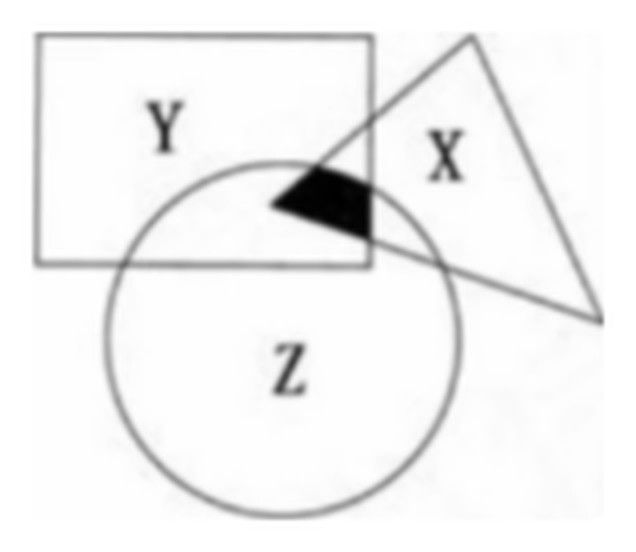
\includegraphics[width=0.20\textwidth]{figures/venn_XYZ_overlap.png}
\end{center}

\ifanswer
\solbegin
\step{设阴影部分的面积是 $x$，则 $290=64+180+160-24-70-36+x$，}
\step{$290=274+x$，$x=16$，故阴影部分的面积是 $16$.}
\solend

\fi

\item 如果集合 $A=\{1,2,3,\cdots,8\}$ 的子集 $B$ 满足：若 $2k\in B$，$k\in\N^{*}$，则 $2k+1\in B$，则称 $B$ 为 $A$ 的“好子集”，$A$ 的“好子集”有 \blankline[2.4em] 个.

\ifanswer
\solbegin
\step{由“好子集”定义得 $2$，$3$ 同时出现，$4$，$5$ 同时出现，$6$，$7$ 同时出现，}
\step{①当集合 $B$ 为空集时，满足题意；}
% 注：原卷此行印作「非空真子集共有 $2^4-1=15$ 种」，与同行算式冲突（$2^4-1=15$ 是**非空子集**数，
%     非空真子集应为 $2^4-2=14$），且与本段①（$B=\varnothing$）合起来恰构成「不含偶数的全体子集」，
%     故按文意订正为「非空子集」（段末总数 $1+15+24+12+2=54$ 不变）。
\step{②当集合 $B$ 中不存在偶数时，$\{1,3,5,7\}$ 的非空子集共有 $2^4-1=15$ 种；}
\step{③当集合 $B$ 中存在 $1$ 个偶数时，三个偶数中选择 $1$ 个，有 $C_3^1=3$ 种，}
\step{剩下 $3$ 个奇数不选，选 $1$ 个、$2$ 个、$3$ 个共有 $2^3=8$ 种，故共有 $24$ 种；}
\step{④当集合 $B$ 中存在 $2$ 个偶数时，三个偶数中选择 $2$ 个，有 $C_3^2=3$ 种，}
\step{剩下 $2$ 个奇数不选，选 $1$ 个、$2$ 个共有 $2^2=4$ 种，故共有 $12$ 种；}
\step{⑤当集合 $B$ 中存在 $3$ 个偶数时，三个偶数中选择 $3$ 个，有 $C_3^3=1$ 种，}
\step{剩下 $1$ 个奇数不选，选 $1$ 个共有 $2^1=2$ 种，故共有 $2$ 种；}
\step{所以 $A$ 的“好子集”共有 $1+15+24+12+2=54$ 种.}
\solend

\fi

\item 已知 $A=\{x\mid x=a^2-b^2,\ a\in\Z,b\in\Z,x\in\N^{*},x\leqslant 40\}$，则集合 $A$ 中共有 \blankline[2.4em] 个元素.

\ifanswer
\solbegin
\step{因为 $(k+1)^2-k^2=2k+1$，所以所有正奇数都属于集合 $A$，}
\step{又 $(2k+2)^2-(2k)^2=8k+4=4(2k+1)$，$(2k+1)^2-(2k-1)^2=8k=4\times 2k$，}
\step{因此所有 $4$ 的整数倍的正整数也属于 $A$，}
\step{若 $x=4k+2$，$k\in\N$，则 $a^2-b^2=(a+b)(a-b)=4k+2=2(2k+1)$，}
\step{则 $a+b$ 和 $a-b$ 中一定是一个取奇数，一个取偶数，}
\step{但是 $a,b\in\Z$ 时，$a+b$ 与 $a-b$ 同奇偶，所以此时无解，}
\step{即所有被 $4$ 除余 $2$ 的正整数都不属于 $A$，}
\step{所以每 $4$ 个数中，有 $3$ 个数属于集合 $A$，则集合 $A$ 中共含 $30$ 个元素.}
\solend

\fi

\item 十个元素组成的集合 $M=\{19,93,-1,0,25,-78,-94,1,17,-2\}$，$M$ 的所有非空子集记为 $M_i$（$i=1,2,\cdots,1023$），每一非空子集中所有元素的乘积记为 $m_i$（$i=1,2,\cdots,1023$），则 $m_1+m_2+\cdots+m_{1023}=$ \blankline[3em].

\ifanswer
\solbegin
\step{因为 $M$ 的所有非空子集为 $M_i$（$i=1,2,\cdots,1023$），这 $1023$ 个子集分成以下几种情况：}
\step{①含 $0$ 的子集有 $512$ 个，这些子集均满足 $m_i=0$；}
\step{②不含 $0$，含 $-1$ 且还含有其它元素的子集有 $255$ 个，}
\step{③不含 $0$，不含 $-1$ 但含有其它元素的子集有 $255$ 个，}
\step{④只含 $-1$ 的子集一个 $\{-1\}$，满足 $m_i=-1$；}
\step{其中②③中的集合是一一对应的，且满足 $m_i$ 对应成相反数，}
\step{故 $m_1+m_2+m_3+\cdots+m_{1023}=512\times 0+255\times 0-1=-1$.}
\solend

\fi

\item 已知 $M=\{(x,y)\mid |xy|=a\}$，$N=\{(x,y)\mid |xy|+1=|x|+|y|\}$，若集合 $M\cap N$ 中的点恰是正八边形的 $8$ 个顶点，则 $a=$ \blankline[2.4em].

\begin{center}
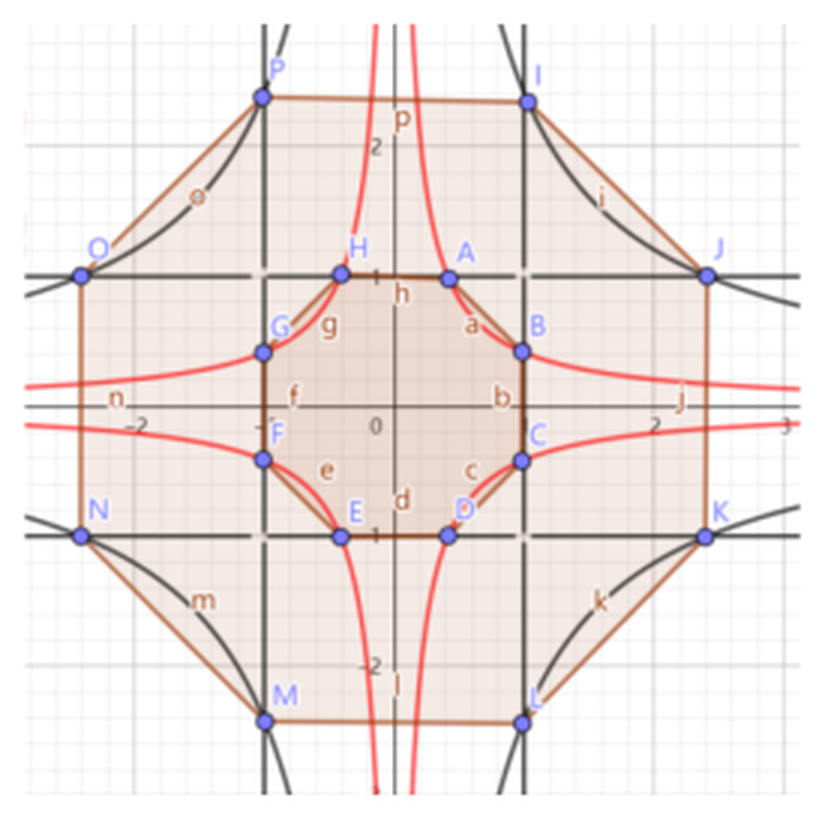
\includegraphics[width=0.44\textwidth]{figures/hyperbola_octagon.png}
\end{center}

\ifanswer
\solbegin
\step{$|xy|=a$ 和 $|xy|+1=|x|+|y|$ 的图像关于坐标轴均对称，只需考虑第一象限即可，}
\step{当 $x>0$，$y>0$ 时，$|xy|+1=|x|+|y|$ 即 $xy+1=x+y$，}
\step{即 $(x-1)(y-1)=0$，}
\step{即 $x=1$ 或 $y=1$，由对称性，作出完整的图像，}
\step{对于 $|xy|=a$，为四段双曲线，}
\step{考虑点 $A(I)(a,1)$，$B(J)(1,a)$，$C(K)(1,-a)$，}
\step{由 $AB=AC$ 得 $\sqrt{(a-1)^2+(1-a)^2}=2a$，解得 $a=\sqrt{2}\pm 1$.}
\solend

\fi

\item 集合 $A$ 是 $\{1,2,3,\cdots,100\}$ 的子集，若 $x\in A$，则 $2x\notin A$，$A$ 中的元素最多有 \blankline[2.4em] 个.

\ifanswer
\solbegin
\step{显然 $51$ 到 $100$ 共 $50$ 个可以，那么从 $1$ 到 $25$ 再 $2$ 倍不会超过 $50$，}
\step{$1$ 到 $25$ 中所有奇数都可以放到子集中，共有 $13$ 个，}
\step{再看偶数，$24=2\times 12$，$22=2\times 11$，$20=2\times 10$，$18=2\times 9$，$16=2\times 8$，}
% 注：末行照原卷抄录。原卷上一行列出 5 个偶数（24、22、20、18、16）而结论写「共有 $50+13+4=67$」，
%     此处的 $4$ 应作「另加 4 个元素」解（穷举验证集合 $A$ 的最大元素数确为 67），非笔误，故不改。
\step{及最后的 $4$，所以，共有 $50+13+4=67$.}
\solend

\fi

\end{enumerate}

\bigsec{二、选择题}

\begin{enumerate}
\setcounter{enumi}{13}

\item 下列各组集合中相等的是（\quad）.

①$P=\{x\mid x=2n,n\in\Z\}$，$Q=\{x\mid x=2(n-1),n\in\Z\}$；

②$P=\{x\mid x^2-1=0\}$，$Q=\left\{x\left|x=\dfrac{1+(-1)^n}{2},n\in\Z\right.\right\}$；

③$P=\{x\mid x=2m+1,m\in\Z\}$，$Q=\{x\mid x=4m\pm 1,m\in\Z\}$；

④$P=\{y\mid y=x^2+1\}$，$Q=\{x\mid y=x^2+1\}$.

\keepwithprev
A. ①②③④\qquad B. ①③\qquad C. ①②④\qquad D. ②④

\ans{B}

\item 如果一个命题的逆命题是真命题，那么这个命题的否命题是（\quad）

\keepwithprev
A. 真命题\qquad B. 假命题

C. 不一定是真命题\qquad D. 不一定是假命题

\ans{A}

\ifanswer
\solbegin
\step{一个命题的逆命题与这个命题的否命题是逆否命题，}
\step{它们的真假性相同，所以逆命题是真命题时，它们的否命题也是真命题. 故选 A.}
\solend

\fi

\item 设 $U$ 表示全集，下列命题中假命题有（\quad）

①若 $A\cap B=U$，则 $A=B=U$；②若 $A\cup B=\varnothing$，则 $A=B=\varnothing$；

③若 $A\cap B=\varnothing$，则 $\overline{A}\cup\overline{B}=U$；④若 $A\cup B=U$，则 $\overline{A}\cap\overline{B}=\varnothing$；

⑤若 $A\subseteq B$，则 $\overline{A}\supseteq\overline{B}$；⑥$\varnothing\in\{\varnothing\}$；⑦$\varnothing\subseteq\{\varnothing\}$.

\keepwithprev
A. $0$\qquad B. $1$\qquad C. $2$\qquad D. $3$

\ans{A}

\ifanswer
\solbegin
\step{全部正确，故选 A.}
\solend

\fi

\end{enumerate}

\bigsec{三、解答题}

\begin{enumerate}
\setcounter{enumi}{16}

\item 已知集合 $A=\{x\mid x^2-3x+2=0\}$，$B=\{x\mid x^2-bx+b-1=0\}$，$C=\{x\mid x^2-cx+2=0\}$.

\begin{enumerate}[label=(\arabic*)]
\item 若 $A\cup B=A$，求实数 $b$ 的值；
\item 若 $A\cap C=C$，求实数 $c$ 的取值范围.
\end{enumerate}

\ifanswer
\solbegin
\stepm{(1)}{$A=\{1,2\}$，$B=\{x\mid(x-1)(x-b+1)=0\}$，}
\step{由 $A\cup B=A$ 得 $b-1=1$ 或 $b-1=2$，所以 $b=2$ 或 $b=3$.}
\stepm{(2)}{由 $A\cap C=C$ 得 $C\subseteq A$，则 $C=\varnothing$ 或 $C=\{1\}$ 或 $C=\{2\}$ 或 $C=\{1,2\}$，}
\step{若 $C=\varnothing$，则 $\Delta=c^2-8<0$，解得 $-2\sqrt{2}<c<2\sqrt{2}$；}
\step{若 $C=\{1\}$，则 $\begin{cases}1+1=c\\ 1\times 1=2\end{cases}$，不可能；}
\step{若 $C=\{2\}$，则 $\begin{cases}2+2=c\\ 2\times 2=2\end{cases}$，不可能；}
\step{若 $C=\{1,2\}$，则 $\begin{cases}1+2=c\\ 1\times 2=2\end{cases}$，符合题意，$c=3$.}
\step{综上所述，$-2\sqrt{2}<c<2\sqrt{2}$ 或 $c=3$.}
\solend

\fi

\ansspace[6]

\item 已知全集 $U=\R$，$A=\{x\mid x^2+px+12=0\}$，$B=\{x\mid x^2-5x+q=0\}$，$\overline{A}\cap B=\{2\}$，求 $p+q$ 的值.

\ifanswer
\solbegin
\step{因为 $\overline{A}\cap B=\{2\}$，所以 $2\in B$，$2\notin A$，}
\step{所以 $2^2-5\times 2+q=0$，解得 $q=6$，$B=\{2,3\}$，}
\step{因为 $\overline{A}\cap B=\{2\}$，$B=\{2,3\}$，所以 $3\in A$，}
\step{所以 $3^2+p\times 3+12=0$，所以 $p=-7$，所以 $p+q=-1$.}
\solend

\fi

\ansspace[5]

\item 求证：方程 $x^2-abx+a+b=0$，$x^2-(a+b)x+ab=0$，其中 $a>2$，$b>2$ 没有公共根.

\ifanswer
\solbegin
\step{假设这两个方程有公共根 $\alpha$，则 $\alpha^2-ab\alpha+(a+b)=0$，$\alpha^2-(a+b)\alpha+ab=0$，}
\step{两式相减得 $(ab-a-b)(\alpha+1)=0$，}
\step{因为 $a>2$，$b>2$，所以 $a-1>1$，$b-1>1$，所以 $(a-1)(b-1)>1$，}
\step{所以 $ab-a-b>0$，所以 $\alpha+1=0$，所以 $\alpha=-1$，}
\step{代入第一个方程，得 $1+ab+a+b=0$，即 $(a+1)(b+1)=0$，}
\step{因为 $a>2$，$b>2$，所以该式不成立，所以这两个方程没有公共根.}
\solend

\fi

\ansspace[9]

% 压轴题：其后已无内容，故作答区全用可丢弃胶水（\ansspace*），并在题目前先量一下版面。
\ansneed{7cm}

\item 若集合 $A$ 具有以下性质：①$0\in A$，$1\in A$；②若 $x$、$y\in A$，则 $x-y\in A$，且 $x\neq 0$ 时，$\dfrac{1}{x}\in A$；则称集合 $A$ 是“好集”.

\begin{enumerate}[label=(\arabic*)]
\item 分别判断集合 $B=\{-1,0,1\}$，有理数集 $\Q$ 是否是“好集”，并说明理由；
\item 设集合 $A$ 是“好集”，求证：若 $x$、$y\in A$，则 $x+y\in A$；
\item 对任意的一个“好集” $A$，分别判断下面命题的真假，并说明理由.

命题 $p$：若 $x$、$y\in A$，则必有 $xy\in A$；

命题 $q$：若 $x$、$y\in A$，且 $x\neq 0$，则必有 $\dfrac{y}{x}\in A$.
\end{enumerate}

\ifanswer
\solbegin
\stepm{(1)}{集合 $B$ 不是“好集”. 理由是：假设集合 $B$ 是“好集”.}
\step{因为 $-1\in B$，$1\in B$，所以 $-1-1=-2\in B$. 这与 $-2\notin B$ 矛盾.}
\step{有理数集 $\Q$ 是“好集”. 因为 $0\in\Q$，$1\in\Q$，}
\step{对任意的 $x$、$y\in\Q$，有 $x-y\in\Q$，且 $x\neq 0$ 时，$\dfrac{1}{x}\in\Q$，}
\step{所以有理数集 $\Q$ 是“好集”.}
\stepm{(2)}{因为集合 $A$ 是“好集”，所以 $0\in A$.}
\step{若 $x$、$y\in A$，则 $0-y\in A$，即 $-y\in A$，所以 $x-(-y)\in A$，即 $x+y\in A$.}
\stepm{(3)}{命题 $p$、$q$ 均为真命题. 理由如下：}
\step{对任意一个“好集” $A$，任取 $x$、$y\in A$，}
\step{若 $x$、$y$ 中有 $0$ 或 $1$ 时，显然 $xy\in A$.}
\step{下设 $x$、$y$ 均不为 $0$，$1$. 由定义得 $x-1$，$\dfrac{1}{x-1}$，$\dfrac{1}{x}\in A$，}
\step{所以 $\dfrac{1}{x-1}-\dfrac{1}{x}\in A$，即 $\dfrac{1}{x(x-1)}\in A$，所以 $x(x-1)\in A$.}
\step{由（2）得 $x(x-1)+x\in A$，即 $x^2\in A$. 同理可得 $y^2\in A$.}
\step{若 $x+y=0$ 或 $x+y=1$，则 $x^2+y^2\in A$.}
\step{若 $x+y\neq 0$ 且 $x+y\neq 1$，则 $(x+y)^2\in A$，}
\step{所以 $2xy=(x+y)^2-x^2-y^2\in A$，所以 $\dfrac{1}{2xy}\in A$，}
\step{由（2）得 $\dfrac{1}{xy}=\dfrac{1}{2xy}+\dfrac{1}{2xy}\in A$，所以 $xy\in A$.}
\step{综上，$xy\in A$，即命题 $p$ 为真命题.}
\step{若 $x$、$y\in A$，且 $x\neq 0$，则 $\dfrac{1}{x}\in A$，}
\step{所以 $\dfrac{y}{x}=y\cdot\dfrac{1}{x}\in A$，即命题 $q$ 为真命题.}
\solend

\fi

\ansspace*[11]

\end{enumerate}

\end{document}
"
%
% 原始材料是微信公众号图文（「魔都数学加油站」），正文为 6 张 PNG 页（1080×1527）。
% 原文本身就是一份**讲评版**——题目下方直接印出【答案】或【解析】，选择题更是把答案
% 直接印在括注里（第 14 题）。试题文字、答案与解析均照原卷录入，未改内容。卷面上的
% 粉色斜水印「魔都数学加油站」属水印，未录入。
%
% 与原卷的排版差异（均已在 README「说明」中交代）：
%   ① 原文自**第 3 题**起（第 1、2 题未在该文中发布），故本稿题号亦自 3 起；
%   ② 原卷未印分节标题，本稿按题型补出「一、填空题」「二、选择题」「三、解答题」三节；
%   ③ 原卷填空、选择题的答案直接印在题目下方（第 14 题印在括注里），本稿统一改为
%      试卷版隐去、答案版以【答案】或【解析】给出，使两版彻底分离；
%   ④ 原卷的 $\R$、$\Q$、$\Z$、$\N$、$\N^{*}$ 时作正体 $R$、$Q$、$Z$、$N$、$N^*$，
%      本稿按全稿惯例统一写作 $\R$、$\Q$、$\Z$、$\N$、$\N^{*}$；
%   ⑤ 原卷中文括注用**半角**括号（第 4 题「(填“真”或“假”)」、第 15 题「是(  )」、
%      第 16 题「有(    )」，均已放大核实），本稿按全稿惯例排全角；
%   ⑥ 第 3 题题干作「$a$ 为**指定**实数」、同题解析作「$a$ 为**给定**的实数」，二者同义，
%      本稿两处均照原卷抄录（未统一）。

% 原卷笔误一处（已逐处放大到能看清字形后核对，本稿按文意订正，并在 README 中写明原委）：
%   ① 第 9 题【解析】② 原卷印「$\{1,3,5,7\}$ 的非空**真**子集共有 $2^4-1=15$ 种」，
%      与同行算式冲突（$2^4-1=15$ 是**非空子集**数，非空真子集应为 $2^4-2=14$），
%      且与本段①（$B=\varnothing$）合起来恰构成「不含偶数的全体子集」，故订正为「非空子集」，
%      段末总数 $1+15+24+12+2=54$ 不变。
%
% 原卷存疑一处（无法确证原意，本稿照抄并加 % 注）：
%   ① 第 12 题【解析】末行「由 $AB=AC$ 得 $\sqrt{(a-1)^2+(1-a)^2}=2a$，解得 $a=\sqrt2\pm1$」——
%      按此式只能解出 $a=\sqrt2-1$（$a=\sqrt2+1$ 处左端 $2$、右端 $4.83$，等式不成立），
%      而其答案 $a=\sqrt2\pm1$ 经数值验证是正确的（两值互为倒数，均使 $M\cap N$ 的 8 个交点按
%      $45^\circ$ 均布）。疑为解析此式笔误，但无法确证原意，本稿照抄原卷、未改。
%      同行上一行的「考虑点 $A(I)(a,1)$，$B(J)(1,a)$，$C(K)(1,-a)$」（点标 I/J/K 与
%      figures/hyperbola_octagon.png 中的标注一一对应）与本行等号右端的 $2a$，均照原卷录入；
%      2026-09-15 回原图逐处放大复核时发现曾误作 $A(1,a)$、$B(a,1)$、$C(-1,a)$ 与「$=2$」，
%      已按原卷订正（见 README「高一14—高一18 专记」）。

\documentclass[a4paper,11pt]{article}
\usepackage{common}

\begin{document}

\examtitlest[3]{2026--2027 年华师大二附中高一上}{集合与逻辑单元练习}

\bigsec{一、填空题}

\begin{enumerate}
\setcounter{enumi}{2}

\item 已知 $a$ 为指定实数，$M=\{x\mid x^2-3x-a^2+2=0\}$ 的非空真子集个数是 \blankline[2.4em].

\ifanswer
\solbegin
\step{集合 $M=\{x\mid x^2-3x-a^2+2=0\}$，$a$ 为给定的实数，}
\step{关于方程 $x^2-3x-a^2+2=0$，因为 $\Delta=(-3)^2-4(2-a^2)=4a^2+1>0$，}
\step{所以方程有两个不同的实根，所以 $M$ 中有两个元素，}
\step{所以集合 $M$ 的非空真子集的个数为 $2^2-2=2$.}
\solend

\fi

\item 判断下列命题的真假：（填“真”或“假”）

（1）任何集合都不是空集的子集 \blankline[2.4em]；

（2）一个有理数与一个无理数的和与积都是无理数 \blankline[2.4em]；

（3）如果一个整数 $n$ 的平方是偶数，那么 $n$ 是偶数 \blankline[2.4em].

\ans{假，假，真}

\item 请写出“如果两个三角形全等，那么它们的面积相等”的逆否命题：\blankline[3em].

\ifanswer
\solbegin
\step{如果两个三角形的面积不相等，则这两个三角形不全等.}
\solend

\fi

\item 已知 $U=\{(x,y)\mid x,y\in\R\}$，$M=\left\{(x,y)\left|\dfrac{y-2}{x-1}=3\right.\right\}$，$N=\{(x,y)\mid y=3x-1\}$，$\overline{M}\cap N=$ \blankline[3em].

\ans{$\{(1,2)\}$}

\item 已知集合 $A=\{x\mid 5x-a\leqslant 0\}$，$B=\{x\mid 6x-b>0\}$，$a$、$b\in\N$，且 $A\cap B\cap\N=\{2,3,4\}$，则整数对 $(a,b)$ 的个数为 \blankline[2.4em].

\ifanswer
\solbegin
\step{$A=\left\{x\left|x\leqslant\dfrac{a}{5}\right.\right\}$，$B=\left\{x\left|x>\dfrac{b}{6}\right.\right\}$，因为 $A\cap B\cap\N=\{2,3,4\}$，}
\step{所以 $4\leqslant\dfrac{a}{5}<5$，$1\leqslant\dfrac{b}{6}<2$，解得 $20\leqslant a<25$，$6\leqslant b<12$，}
\step{又 $a$、$b\in\N$，所以 $a=20$，$21$，$22$，$23$，$24$，$b=6$，$7$，$8$，$9$，$10$，$11$，}
\step{则整数对 $(a,b)$ 的个数为 $30$.}
\solend

\fi

\item 如图所示，$X$、$Y$、$Z$ 分别是面积为 $64$、$180$、$160$ 的三张不同形状的纸片，它们部分重叠放在一起盖在桌面上，总共盖住的面积为 $290$，且 $X$ 与 $Y$、$Y$ 与 $Z$、$Z$ 与 $X$ 重叠部分面积分别为 $24$、$70$、$36$，问阴影部分的面积是 \blankline[2.4em].

\begin{center}
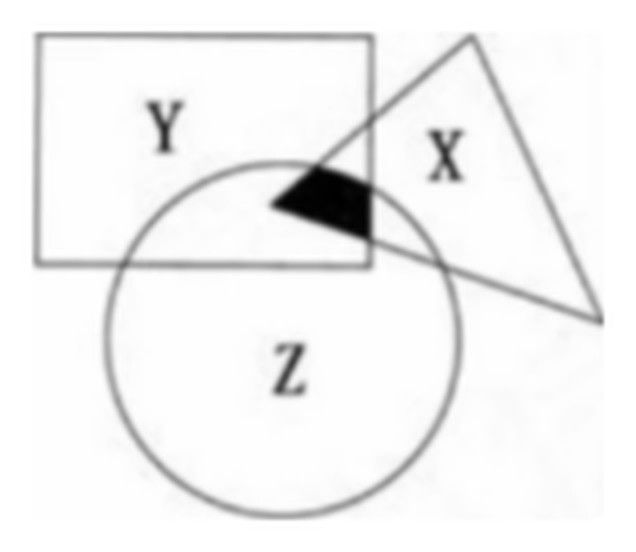
\includegraphics[width=0.20\textwidth]{figures/venn_XYZ_overlap.png}
\end{center}

\ifanswer
\solbegin
\step{设阴影部分的面积是 $x$，则 $290=64+180+160-24-70-36+x$，}
\step{$290=274+x$，$x=16$，故阴影部分的面积是 $16$.}
\solend

\fi

\item 如果集合 $A=\{1,2,3,\cdots,8\}$ 的子集 $B$ 满足：若 $2k\in B$，$k\in\N^{*}$，则 $2k+1\in B$，则称 $B$ 为 $A$ 的“好子集”，$A$ 的“好子集”有 \blankline[2.4em] 个.

\ifanswer
\solbegin
\step{由“好子集”定义得 $2$，$3$ 同时出现，$4$，$5$ 同时出现，$6$，$7$ 同时出现，}
\step{①当集合 $B$ 为空集时，满足题意；}
% 注：原卷此行印作「非空真子集共有 $2^4-1=15$ 种」，与同行算式冲突（$2^4-1=15$ 是**非空子集**数，
%     非空真子集应为 $2^4-2=14$），且与本段①（$B=\varnothing$）合起来恰构成「不含偶数的全体子集」，
%     故按文意订正为「非空子集」（段末总数 $1+15+24+12+2=54$ 不变）。
\step{②当集合 $B$ 中不存在偶数时，$\{1,3,5,7\}$ 的非空子集共有 $2^4-1=15$ 种；}
\step{③当集合 $B$ 中存在 $1$ 个偶数时，三个偶数中选择 $1$ 个，有 $C_3^1=3$ 种，}
\step{剩下 $3$ 个奇数不选，选 $1$ 个、$2$ 个、$3$ 个共有 $2^3=8$ 种，故共有 $24$ 种；}
\step{④当集合 $B$ 中存在 $2$ 个偶数时，三个偶数中选择 $2$ 个，有 $C_3^2=3$ 种，}
\step{剩下 $2$ 个奇数不选，选 $1$ 个、$2$ 个共有 $2^2=4$ 种，故共有 $12$ 种；}
\step{⑤当集合 $B$ 中存在 $3$ 个偶数时，三个偶数中选择 $3$ 个，有 $C_3^3=1$ 种，}
\step{剩下 $1$ 个奇数不选，选 $1$ 个共有 $2^1=2$ 种，故共有 $2$ 种；}
\step{所以 $A$ 的“好子集”共有 $1+15+24+12+2=54$ 种.}
\solend

\fi

\item 已知 $A=\{x\mid x=a^2-b^2,\ a\in\Z,b\in\Z,x\in\N^{*},x\leqslant 40\}$，则集合 $A$ 中共有 \blankline[2.4em] 个元素.

\ifanswer
\solbegin
\step{因为 $(k+1)^2-k^2=2k+1$，所以所有正奇数都属于集合 $A$，}
\step{又 $(2k+2)^2-(2k)^2=8k+4=4(2k+1)$，$(2k+1)^2-(2k-1)^2=8k=4\times 2k$，}
\step{因此所有 $4$ 的整数倍的正整数也属于 $A$，}
\step{若 $x=4k+2$，$k\in\N$，则 $a^2-b^2=(a+b)(a-b)=4k+2=2(2k+1)$，}
\step{则 $a+b$ 和 $a-b$ 中一定是一个取奇数，一个取偶数，}
\step{但是 $a,b\in\Z$ 时，$a+b$ 与 $a-b$ 同奇偶，所以此时无解，}
\step{即所有被 $4$ 除余 $2$ 的正整数都不属于 $A$，}
\step{所以每 $4$ 个数中，有 $3$ 个数属于集合 $A$，则集合 $A$ 中共含 $30$ 个元素.}
\solend

\fi

\item 十个元素组成的集合 $M=\{19,93,-1,0,25,-78,-94,1,17,-2\}$，$M$ 的所有非空子集记为 $M_i$（$i=1,2,\cdots,1023$），每一非空子集中所有元素的乘积记为 $m_i$（$i=1,2,\cdots,1023$），则 $m_1+m_2+\cdots+m_{1023}=$ \blankline[3em].

\ifanswer
\solbegin
\step{因为 $M$ 的所有非空子集为 $M_i$（$i=1,2,\cdots,1023$），这 $1023$ 个子集分成以下几种情况：}
\step{①含 $0$ 的子集有 $512$ 个，这些子集均满足 $m_i=0$；}
\step{②不含 $0$，含 $-1$ 且还含有其它元素的子集有 $255$ 个，}
\step{③不含 $0$，不含 $-1$ 但含有其它元素的子集有 $255$ 个，}
\step{④只含 $-1$ 的子集一个 $\{-1\}$，满足 $m_i=-1$；}
\step{其中②③中的集合是一一对应的，且满足 $m_i$ 对应成相反数，}
\step{故 $m_1+m_2+m_3+\cdots+m_{1023}=512\times 0+255\times 0-1=-1$.}
\solend

\fi

\item 已知 $M=\{(x,y)\mid |xy|=a\}$，$N=\{(x,y)\mid |xy|+1=|x|+|y|\}$，若集合 $M\cap N$ 中的点恰是正八边形的 $8$ 个顶点，则 $a=$ \blankline[2.4em].

\begin{center}
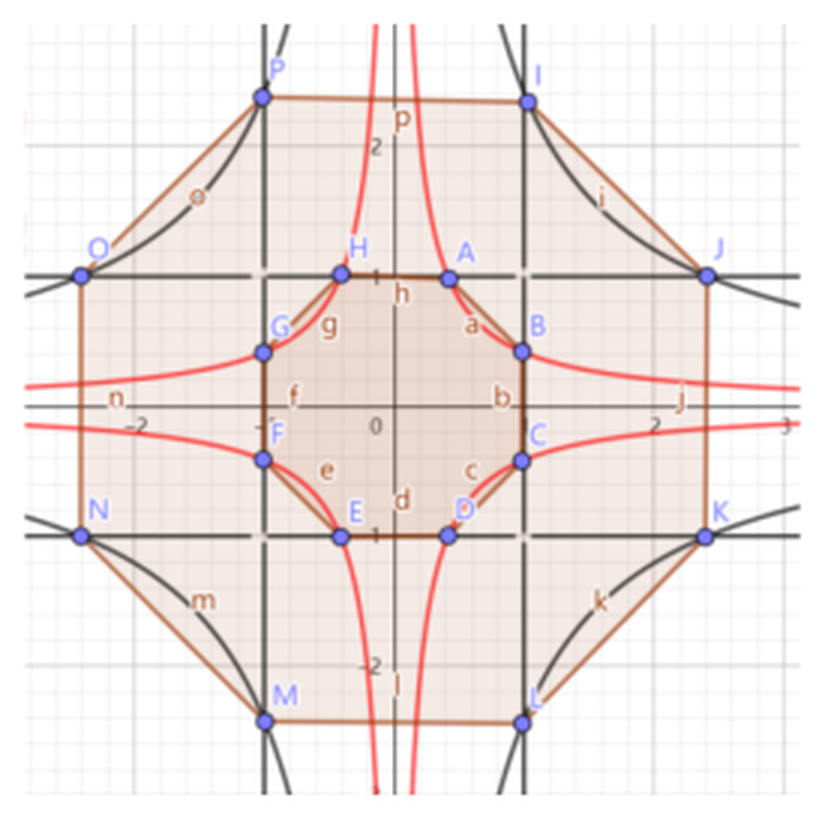
\includegraphics[width=0.44\textwidth]{figures/hyperbola_octagon.png}
\end{center}

\ifanswer
\solbegin
\step{$|xy|=a$ 和 $|xy|+1=|x|+|y|$ 的图像关于坐标轴均对称，只需考虑第一象限即可，}
\step{当 $x>0$，$y>0$ 时，$|xy|+1=|x|+|y|$ 即 $xy+1=x+y$，}
\step{即 $(x-1)(y-1)=0$，}
\step{即 $x=1$ 或 $y=1$，由对称性，作出完整的图像，}
\step{对于 $|xy|=a$，为四段双曲线，}
\step{考虑点 $A(I)(a,1)$，$B(J)(1,a)$，$C(K)(1,-a)$，}
\step{由 $AB=AC$ 得 $\sqrt{(a-1)^2+(1-a)^2}=2a$，解得 $a=\sqrt{2}\pm 1$.}
\solend

\fi

\item 集合 $A$ 是 $\{1,2,3,\cdots,100\}$ 的子集，若 $x\in A$，则 $2x\notin A$，$A$ 中的元素最多有 \blankline[2.4em] 个.

\ifanswer
\solbegin
\step{显然 $51$ 到 $100$ 共 $50$ 个可以，那么从 $1$ 到 $25$ 再 $2$ 倍不会超过 $50$，}
\step{$1$ 到 $25$ 中所有奇数都可以放到子集中，共有 $13$ 个，}
\step{再看偶数，$24=2\times 12$，$22=2\times 11$，$20=2\times 10$，$18=2\times 9$，$16=2\times 8$，}
% 注：末行照原卷抄录。原卷上一行列出 5 个偶数（24、22、20、18、16）而结论写「共有 $50+13+4=67$」，
%     此处的 $4$ 应作「另加 4 个元素」解（穷举验证集合 $A$ 的最大元素数确为 67），非笔误，故不改。
\step{及最后的 $4$，所以，共有 $50+13+4=67$.}
\solend

\fi

\end{enumerate}

\bigsec{二、选择题}

\begin{enumerate}
\setcounter{enumi}{13}

\item 下列各组集合中相等的是（\quad）.

①$P=\{x\mid x=2n,n\in\Z\}$，$Q=\{x\mid x=2(n-1),n\in\Z\}$；

②$P=\{x\mid x^2-1=0\}$，$Q=\left\{x\left|x=\dfrac{1+(-1)^n}{2},n\in\Z\right.\right\}$；

③$P=\{x\mid x=2m+1,m\in\Z\}$，$Q=\{x\mid x=4m\pm 1,m\in\Z\}$；

④$P=\{y\mid y=x^2+1\}$，$Q=\{x\mid y=x^2+1\}$.

\keepwithprev
A. ①②③④\qquad B. ①③\qquad C. ①②④\qquad D. ②④

\ans{B}

\item 如果一个命题的逆命题是真命题，那么这个命题的否命题是（\quad）

\keepwithprev
A. 真命题\qquad B. 假命题

C. 不一定是真命题\qquad D. 不一定是假命题

\ans{A}

\ifanswer
\solbegin
\step{一个命题的逆命题与这个命题的否命题是逆否命题，}
\step{它们的真假性相同，所以逆命题是真命题时，它们的否命题也是真命题. 故选 A.}
\solend

\fi

\item 设 $U$ 表示全集，下列命题中假命题有（\quad）

①若 $A\cap B=U$，则 $A=B=U$；②若 $A\cup B=\varnothing$，则 $A=B=\varnothing$；

③若 $A\cap B=\varnothing$，则 $\overline{A}\cup\overline{B}=U$；④若 $A\cup B=U$，则 $\overline{A}\cap\overline{B}=\varnothing$；

⑤若 $A\subseteq B$，则 $\overline{A}\supseteq\overline{B}$；⑥$\varnothing\in\{\varnothing\}$；⑦$\varnothing\subseteq\{\varnothing\}$.

\keepwithprev
A. $0$\qquad B. $1$\qquad C. $2$\qquad D. $3$

\ans{A}

\ifanswer
\solbegin
\step{全部正确，故选 A.}
\solend

\fi

\end{enumerate}

\bigsec{三、解答题}

\begin{enumerate}
\setcounter{enumi}{16}

\item 已知集合 $A=\{x\mid x^2-3x+2=0\}$，$B=\{x\mid x^2-bx+b-1=0\}$，$C=\{x\mid x^2-cx+2=0\}$.

\begin{enumerate}[label=(\arabic*)]
\item 若 $A\cup B=A$，求实数 $b$ 的值；
\item 若 $A\cap C=C$，求实数 $c$ 的取值范围.
\end{enumerate}

\ifanswer
\solbegin
\stepm{(1)}{$A=\{1,2\}$，$B=\{x\mid(x-1)(x-b+1)=0\}$，}
\step{由 $A\cup B=A$ 得 $b-1=1$ 或 $b-1=2$，所以 $b=2$ 或 $b=3$.}
\stepm{(2)}{由 $A\cap C=C$ 得 $C\subseteq A$，则 $C=\varnothing$ 或 $C=\{1\}$ 或 $C=\{2\}$ 或 $C=\{1,2\}$，}
\step{若 $C=\varnothing$，则 $\Delta=c^2-8<0$，解得 $-2\sqrt{2}<c<2\sqrt{2}$；}
\step{若 $C=\{1\}$，则 $\begin{cases}1+1=c\\ 1\times 1=2\end{cases}$，不可能；}
\step{若 $C=\{2\}$，则 $\begin{cases}2+2=c\\ 2\times 2=2\end{cases}$，不可能；}
\step{若 $C=\{1,2\}$，则 $\begin{cases}1+2=c\\ 1\times 2=2\end{cases}$，符合题意，$c=3$.}
\step{综上所述，$-2\sqrt{2}<c<2\sqrt{2}$ 或 $c=3$.}
\solend

\fi

\ansspace[6]

\item 已知全集 $U=\R$，$A=\{x\mid x^2+px+12=0\}$，$B=\{x\mid x^2-5x+q=0\}$，$\overline{A}\cap B=\{2\}$，求 $p+q$ 的值.

\ifanswer
\solbegin
\step{因为 $\overline{A}\cap B=\{2\}$，所以 $2\in B$，$2\notin A$，}
\step{所以 $2^2-5\times 2+q=0$，解得 $q=6$，$B=\{2,3\}$，}
\step{因为 $\overline{A}\cap B=\{2\}$，$B=\{2,3\}$，所以 $3\in A$，}
\step{所以 $3^2+p\times 3+12=0$，所以 $p=-7$，所以 $p+q=-1$.}
\solend

\fi

\ansspace[5]

\item 求证：方程 $x^2-abx+a+b=0$，$x^2-(a+b)x+ab=0$，其中 $a>2$，$b>2$ 没有公共根.

\ifanswer
\solbegin
\step{假设这两个方程有公共根 $\alpha$，则 $\alpha^2-ab\alpha+(a+b)=0$，$\alpha^2-(a+b)\alpha+ab=0$，}
\step{两式相减得 $(ab-a-b)(\alpha+1)=0$，}
\step{因为 $a>2$，$b>2$，所以 $a-1>1$，$b-1>1$，所以 $(a-1)(b-1)>1$，}
\step{所以 $ab-a-b>0$，所以 $\alpha+1=0$，所以 $\alpha=-1$，}
\step{代入第一个方程，得 $1+ab+a+b=0$，即 $(a+1)(b+1)=0$，}
\step{因为 $a>2$，$b>2$，所以该式不成立，所以这两个方程没有公共根.}
\solend

\fi

\ansspace[9]

% 压轴题：其后已无内容，故作答区全用可丢弃胶水（\ansspace*），并在题目前先量一下版面。
\ansneed{7cm}

\item 若集合 $A$ 具有以下性质：①$0\in A$，$1\in A$；②若 $x$、$y\in A$，则 $x-y\in A$，且 $x\neq 0$ 时，$\dfrac{1}{x}\in A$；则称集合 $A$ 是“好集”.

\begin{enumerate}[label=(\arabic*)]
\item 分别判断集合 $B=\{-1,0,1\}$，有理数集 $\Q$ 是否是“好集”，并说明理由；
\item 设集合 $A$ 是“好集”，求证：若 $x$、$y\in A$，则 $x+y\in A$；
\item 对任意的一个“好集” $A$，分别判断下面命题的真假，并说明理由.

命题 $p$：若 $x$、$y\in A$，则必有 $xy\in A$；

命题 $q$：若 $x$、$y\in A$，且 $x\neq 0$，则必有 $\dfrac{y}{x}\in A$.
\end{enumerate}

\ifanswer
\solbegin
\stepm{(1)}{集合 $B$ 不是“好集”. 理由是：假设集合 $B$ 是“好集”.}
\step{因为 $-1\in B$，$1\in B$，所以 $-1-1=-2\in B$. 这与 $-2\notin B$ 矛盾.}
\step{有理数集 $\Q$ 是“好集”. 因为 $0\in\Q$，$1\in\Q$，}
\step{对任意的 $x$、$y\in\Q$，有 $x-y\in\Q$，且 $x\neq 0$ 时，$\dfrac{1}{x}\in\Q$，}
\step{所以有理数集 $\Q$ 是“好集”.}
\stepm{(2)}{因为集合 $A$ 是“好集”，所以 $0\in A$.}
\step{若 $x$、$y\in A$，则 $0-y\in A$，即 $-y\in A$，所以 $x-(-y)\in A$，即 $x+y\in A$.}
\stepm{(3)}{命题 $p$、$q$ 均为真命题. 理由如下：}
\step{对任意一个“好集” $A$，任取 $x$、$y\in A$，}
\step{若 $x$、$y$ 中有 $0$ 或 $1$ 时，显然 $xy\in A$.}
\step{下设 $x$、$y$ 均不为 $0$，$1$. 由定义得 $x-1$，$\dfrac{1}{x-1}$，$\dfrac{1}{x}\in A$，}
\step{所以 $\dfrac{1}{x-1}-\dfrac{1}{x}\in A$，即 $\dfrac{1}{x(x-1)}\in A$，所以 $x(x-1)\in A$.}
\step{由（2）得 $x(x-1)+x\in A$，即 $x^2\in A$. 同理可得 $y^2\in A$.}
\step{若 $x+y=0$ 或 $x+y=1$，则 $x^2+y^2\in A$.}
\step{若 $x+y\neq 0$ 且 $x+y\neq 1$，则 $(x+y)^2\in A$，}
\step{所以 $2xy=(x+y)^2-x^2-y^2\in A$，所以 $\dfrac{1}{2xy}\in A$，}
\step{由（2）得 $\dfrac{1}{xy}=\dfrac{1}{2xy}+\dfrac{1}{2xy}\in A$，所以 $xy\in A$.}
\step{综上，$xy\in A$，即命题 $p$ 为真命题.}
\step{若 $x$、$y\in A$，且 $x\neq 0$，则 $\dfrac{1}{x}\in A$，}
\step{所以 $\dfrac{y}{x}=y\cdot\dfrac{1}{x}\in A$，即命题 $q$ 为真命题.}
\solend

\fi

\ansspace*[11]

\end{enumerate}

\end{document}
"
%
% 原始材料是微信公众号图文（「魔都数学加油站」），正文为 6 张 PNG 页（1080×1527）。
% 原文本身就是一份**讲评版**——题目下方直接印出【答案】或【解析】，选择题更是把答案
% 直接印在括注里（第 14 题）。试题文字、答案与解析均照原卷录入，未改内容。卷面上的
% 粉色斜水印「魔都数学加油站」属水印，未录入。
%
% 与原卷的排版差异（均已在 README「说明」中交代）：
%   ① 原文自**第 3 题**起（第 1、2 题未在该文中发布），故本稿题号亦自 3 起；
%   ② 原卷未印分节标题，本稿按题型补出「一、填空题」「二、选择题」「三、解答题」三节；
%   ③ 原卷填空、选择题的答案直接印在题目下方（第 14 题印在括注里），本稿统一改为
%      试卷版隐去、答案版以【答案】或【解析】给出，使两版彻底分离；
%   ④ 原卷的 $\R$、$\Q$、$\Z$、$\N$、$\N^{*}$ 时作正体 $R$、$Q$、$Z$、$N$、$N^*$，
%      本稿按全稿惯例统一写作 $\R$、$\Q$、$\Z$、$\N$、$\N^{*}$；
%   ⑤ 原卷中文括注用**半角**括号（第 4 题「(填“真”或“假”)」、第 15 题「是(  )」、
%      第 16 题「有(    )」，均已放大核实），本稿按全稿惯例排全角；
%   ⑥ 第 3 题题干作「$a$ 为**指定**实数」、同题解析作「$a$ 为**给定**的实数」，二者同义，
%      本稿两处均照原卷抄录（未统一）。

% 原卷笔误一处（已逐处放大到能看清字形后核对，本稿按文意订正，并在 README 中写明原委）：
%   ① 第 9 题【解析】② 原卷印「$\{1,3,5,7\}$ 的非空**真**子集共有 $2^4-1=15$ 种」，
%      与同行算式冲突（$2^4-1=15$ 是**非空子集**数，非空真子集应为 $2^4-2=14$），
%      且与本段①（$B=\varnothing$）合起来恰构成「不含偶数的全体子集」，故订正为「非空子集」，
%      段末总数 $1+15+24+12+2=54$ 不变。
%
% 原卷存疑一处（无法确证原意，本稿照抄并加 % 注）：
%   ① 第 12 题【解析】末行「由 $AB=AC$ 得 $\sqrt{(a-1)^2+(1-a)^2}=2a$，解得 $a=\sqrt2\pm1$」——
%      按此式只能解出 $a=\sqrt2-1$（$a=\sqrt2+1$ 处左端 $2$、右端 $4.83$，等式不成立），
%      而其答案 $a=\sqrt2\pm1$ 经数值验证是正确的（两值互为倒数，均使 $M\cap N$ 的 8 个交点按
%      $45^\circ$ 均布）。疑为解析此式笔误，但无法确证原意，本稿照抄原卷、未改。
%      同行上一行的「考虑点 $A(I)(a,1)$，$B(J)(1,a)$，$C(K)(1,-a)$」（点标 I/J/K 与
%      figures/hyperbola_octagon.png 中的标注一一对应）与本行等号右端的 $2a$，均照原卷录入；
%      2026-09-15 回原图逐处放大复核时发现曾误作 $A(1,a)$、$B(a,1)$、$C(-1,a)$ 与「$=2$」，
%      已按原卷订正（见 README「高一14—高一18 专记」）。

\documentclass[a4paper,11pt]{article}
\usepackage{common}

\begin{document}

\examtitlest[3]{2026--2027 年华师大二附中高一上}{集合与逻辑单元练习}

\bigsec{一、填空题}

\begin{enumerate}
\setcounter{enumi}{2}

\item 已知 $a$ 为指定实数，$M=\{x\mid x^2-3x-a^2+2=0\}$ 的非空真子集个数是 \blankline[2.4em].

\ifanswer
\solbegin
\step{集合 $M=\{x\mid x^2-3x-a^2+2=0\}$，$a$ 为给定的实数，}
\step{关于方程 $x^2-3x-a^2+2=0$，因为 $\Delta=(-3)^2-4(2-a^2)=4a^2+1>0$，}
\step{所以方程有两个不同的实根，所以 $M$ 中有两个元素，}
\step{所以集合 $M$ 的非空真子集的个数为 $2^2-2=2$.}
\solend

\fi

\item 判断下列命题的真假：（填“真”或“假”）

（1）任何集合都不是空集的子集 \blankline[2.4em]；

（2）一个有理数与一个无理数的和与积都是无理数 \blankline[2.4em]；

（3）如果一个整数 $n$ 的平方是偶数，那么 $n$ 是偶数 \blankline[2.4em].

\ans{假，假，真}

\item 请写出“如果两个三角形全等，那么它们的面积相等”的逆否命题：\blankline[3em].

\ifanswer
\solbegin
\step{如果两个三角形的面积不相等，则这两个三角形不全等.}
\solend

\fi

\item 已知 $U=\{(x,y)\mid x,y\in\R\}$，$M=\left\{(x,y)\left|\dfrac{y-2}{x-1}=3\right.\right\}$，$N=\{(x,y)\mid y=3x-1\}$，$\overline{M}\cap N=$ \blankline[3em].

\ans{$\{(1,2)\}$}

\item 已知集合 $A=\{x\mid 5x-a\leqslant 0\}$，$B=\{x\mid 6x-b>0\}$，$a$、$b\in\N$，且 $A\cap B\cap\N=\{2,3,4\}$，则整数对 $(a,b)$ 的个数为 \blankline[2.4em].

\ifanswer
\solbegin
\step{$A=\left\{x\left|x\leqslant\dfrac{a}{5}\right.\right\}$，$B=\left\{x\left|x>\dfrac{b}{6}\right.\right\}$，因为 $A\cap B\cap\N=\{2,3,4\}$，}
\step{所以 $4\leqslant\dfrac{a}{5}<5$，$1\leqslant\dfrac{b}{6}<2$，解得 $20\leqslant a<25$，$6\leqslant b<12$，}
\step{又 $a$、$b\in\N$，所以 $a=20$，$21$，$22$，$23$，$24$，$b=6$，$7$，$8$，$9$，$10$，$11$，}
\step{则整数对 $(a,b)$ 的个数为 $30$.}
\solend

\fi

\item 如图所示，$X$、$Y$、$Z$ 分别是面积为 $64$、$180$、$160$ 的三张不同形状的纸片，它们部分重叠放在一起盖在桌面上，总共盖住的面积为 $290$，且 $X$ 与 $Y$、$Y$ 与 $Z$、$Z$ 与 $X$ 重叠部分面积分别为 $24$、$70$、$36$，问阴影部分的面积是 \blankline[2.4em].

\begin{center}
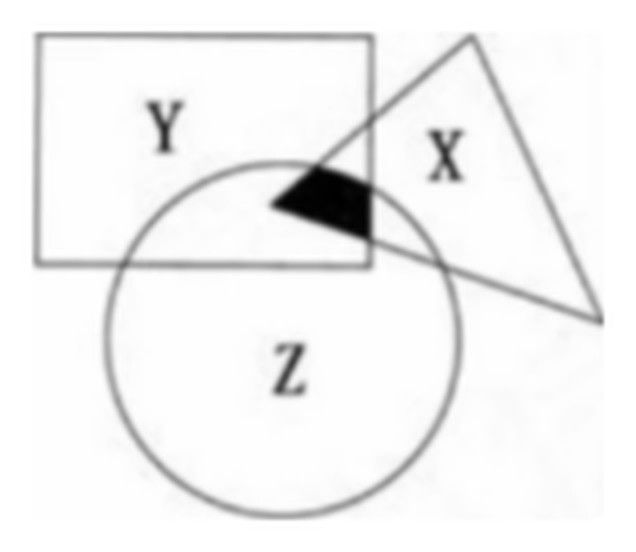
\includegraphics[width=0.20\textwidth]{figures/venn_XYZ_overlap.png}
\end{center}

\ifanswer
\solbegin
\step{设阴影部分的面积是 $x$，则 $290=64+180+160-24-70-36+x$，}
\step{$290=274+x$，$x=16$，故阴影部分的面积是 $16$.}
\solend

\fi

\item 如果集合 $A=\{1,2,3,\cdots,8\}$ 的子集 $B$ 满足：若 $2k\in B$，$k\in\N^{*}$，则 $2k+1\in B$，则称 $B$ 为 $A$ 的“好子集”，$A$ 的“好子集”有 \blankline[2.4em] 个.

\ifanswer
\solbegin
\step{由“好子集”定义得 $2$，$3$ 同时出现，$4$，$5$ 同时出现，$6$，$7$ 同时出现，}
\step{①当集合 $B$ 为空集时，满足题意；}
% 注：原卷此行印作「非空真子集共有 $2^4-1=15$ 种」，与同行算式冲突（$2^4-1=15$ 是**非空子集**数，
%     非空真子集应为 $2^4-2=14$），且与本段①（$B=\varnothing$）合起来恰构成「不含偶数的全体子集」，
%     故按文意订正为「非空子集」（段末总数 $1+15+24+12+2=54$ 不变）。
\step{②当集合 $B$ 中不存在偶数时，$\{1,3,5,7\}$ 的非空子集共有 $2^4-1=15$ 种；}
\step{③当集合 $B$ 中存在 $1$ 个偶数时，三个偶数中选择 $1$ 个，有 $C_3^1=3$ 种，}
\step{剩下 $3$ 个奇数不选，选 $1$ 个、$2$ 个、$3$ 个共有 $2^3=8$ 种，故共有 $24$ 种；}
\step{④当集合 $B$ 中存在 $2$ 个偶数时，三个偶数中选择 $2$ 个，有 $C_3^2=3$ 种，}
\step{剩下 $2$ 个奇数不选，选 $1$ 个、$2$ 个共有 $2^2=4$ 种，故共有 $12$ 种；}
\step{⑤当集合 $B$ 中存在 $3$ 个偶数时，三个偶数中选择 $3$ 个，有 $C_3^3=1$ 种，}
\step{剩下 $1$ 个奇数不选，选 $1$ 个共有 $2^1=2$ 种，故共有 $2$ 种；}
\step{所以 $A$ 的“好子集”共有 $1+15+24+12+2=54$ 种.}
\solend

\fi

\item 已知 $A=\{x\mid x=a^2-b^2,\ a\in\Z,b\in\Z,x\in\N^{*},x\leqslant 40\}$，则集合 $A$ 中共有 \blankline[2.4em] 个元素.

\ifanswer
\solbegin
\step{因为 $(k+1)^2-k^2=2k+1$，所以所有正奇数都属于集合 $A$，}
\step{又 $(2k+2)^2-(2k)^2=8k+4=4(2k+1)$，$(2k+1)^2-(2k-1)^2=8k=4\times 2k$，}
\step{因此所有 $4$ 的整数倍的正整数也属于 $A$，}
\step{若 $x=4k+2$，$k\in\N$，则 $a^2-b^2=(a+b)(a-b)=4k+2=2(2k+1)$，}
\step{则 $a+b$ 和 $a-b$ 中一定是一个取奇数，一个取偶数，}
\step{但是 $a,b\in\Z$ 时，$a+b$ 与 $a-b$ 同奇偶，所以此时无解，}
\step{即所有被 $4$ 除余 $2$ 的正整数都不属于 $A$，}
\step{所以每 $4$ 个数中，有 $3$ 个数属于集合 $A$，则集合 $A$ 中共含 $30$ 个元素.}
\solend

\fi

\item 十个元素组成的集合 $M=\{19,93,-1,0,25,-78,-94,1,17,-2\}$，$M$ 的所有非空子集记为 $M_i$（$i=1,2,\cdots,1023$），每一非空子集中所有元素的乘积记为 $m_i$（$i=1,2,\cdots,1023$），则 $m_1+m_2+\cdots+m_{1023}=$ \blankline[3em].

\ifanswer
\solbegin
\step{因为 $M$ 的所有非空子集为 $M_i$（$i=1,2,\cdots,1023$），这 $1023$ 个子集分成以下几种情况：}
\step{①含 $0$ 的子集有 $512$ 个，这些子集均满足 $m_i=0$；}
\step{②不含 $0$，含 $-1$ 且还含有其它元素的子集有 $255$ 个，}
\step{③不含 $0$，不含 $-1$ 但含有其它元素的子集有 $255$ 个，}
\step{④只含 $-1$ 的子集一个 $\{-1\}$，满足 $m_i=-1$；}
\step{其中②③中的集合是一一对应的，且满足 $m_i$ 对应成相反数，}
\step{故 $m_1+m_2+m_3+\cdots+m_{1023}=512\times 0+255\times 0-1=-1$.}
\solend

\fi

\item 已知 $M=\{(x,y)\mid |xy|=a\}$，$N=\{(x,y)\mid |xy|+1=|x|+|y|\}$，若集合 $M\cap N$ 中的点恰是正八边形的 $8$ 个顶点，则 $a=$ \blankline[2.4em].

\begin{center}
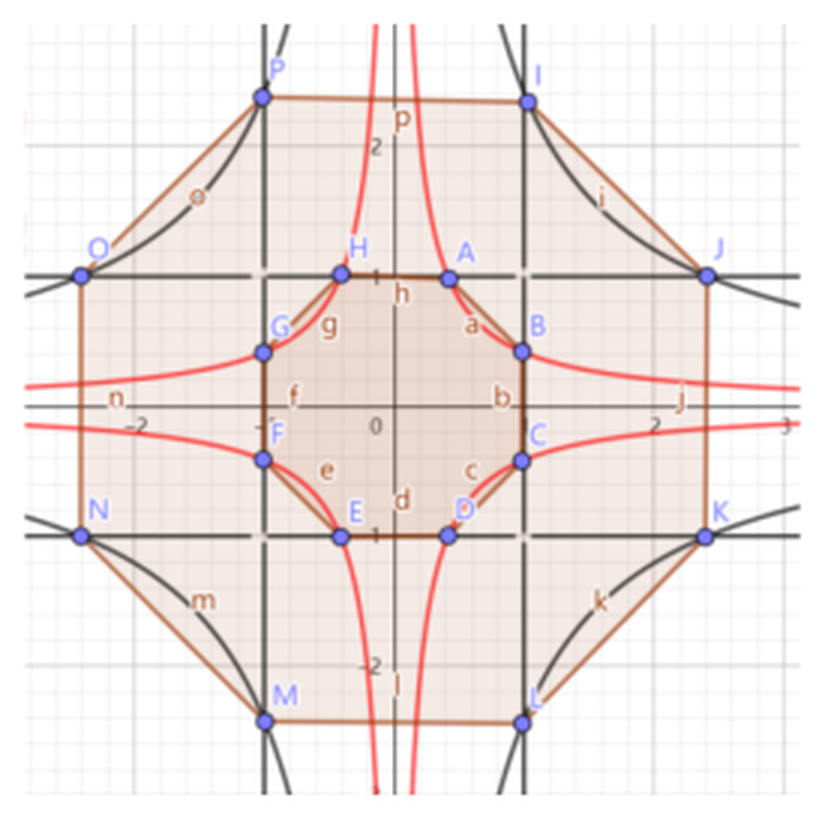
\includegraphics[width=0.44\textwidth]{figures/hyperbola_octagon.png}
\end{center}

\ifanswer
\solbegin
\step{$|xy|=a$ 和 $|xy|+1=|x|+|y|$ 的图像关于坐标轴均对称，只需考虑第一象限即可，}
\step{当 $x>0$，$y>0$ 时，$|xy|+1=|x|+|y|$ 即 $xy+1=x+y$，}
\step{即 $(x-1)(y-1)=0$，}
\step{即 $x=1$ 或 $y=1$，由对称性，作出完整的图像，}
\step{对于 $|xy|=a$，为四段双曲线，}
\step{考虑点 $A(I)(a,1)$，$B(J)(1,a)$，$C(K)(1,-a)$，}
\step{由 $AB=AC$ 得 $\sqrt{(a-1)^2+(1-a)^2}=2a$，解得 $a=\sqrt{2}\pm 1$.}
\solend

\fi

\item 集合 $A$ 是 $\{1,2,3,\cdots,100\}$ 的子集，若 $x\in A$，则 $2x\notin A$，$A$ 中的元素最多有 \blankline[2.4em] 个.

\ifanswer
\solbegin
\step{显然 $51$ 到 $100$ 共 $50$ 个可以，那么从 $1$ 到 $25$ 再 $2$ 倍不会超过 $50$，}
\step{$1$ 到 $25$ 中所有奇数都可以放到子集中，共有 $13$ 个，}
\step{再看偶数，$24=2\times 12$，$22=2\times 11$，$20=2\times 10$，$18=2\times 9$，$16=2\times 8$，}
% 注：末行照原卷抄录。原卷上一行列出 5 个偶数（24、22、20、18、16）而结论写「共有 $50+13+4=67$」，
%     此处的 $4$ 应作「另加 4 个元素」解（穷举验证集合 $A$ 的最大元素数确为 67），非笔误，故不改。
\step{及最后的 $4$，所以，共有 $50+13+4=67$.}
\solend

\fi

\end{enumerate}

\bigsec{二、选择题}

\begin{enumerate}
\setcounter{enumi}{13}

\item 下列各组集合中相等的是（\quad）.

①$P=\{x\mid x=2n,n\in\Z\}$，$Q=\{x\mid x=2(n-1),n\in\Z\}$；

②$P=\{x\mid x^2-1=0\}$，$Q=\left\{x\left|x=\dfrac{1+(-1)^n}{2},n\in\Z\right.\right\}$；

③$P=\{x\mid x=2m+1,m\in\Z\}$，$Q=\{x\mid x=4m\pm 1,m\in\Z\}$；

④$P=\{y\mid y=x^2+1\}$，$Q=\{x\mid y=x^2+1\}$.

\keepwithprev
A. ①②③④\qquad B. ①③\qquad C. ①②④\qquad D. ②④

\ans{B}

\item 如果一个命题的逆命题是真命题，那么这个命题的否命题是（\quad）

\keepwithprev
A. 真命题\qquad B. 假命题

C. 不一定是真命题\qquad D. 不一定是假命题

\ans{A}

\ifanswer
\solbegin
\step{一个命题的逆命题与这个命题的否命题是逆否命题，}
\step{它们的真假性相同，所以逆命题是真命题时，它们的否命题也是真命题. 故选 A.}
\solend

\fi

\item 设 $U$ 表示全集，下列命题中假命题有（\quad）

①若 $A\cap B=U$，则 $A=B=U$；②若 $A\cup B=\varnothing$，则 $A=B=\varnothing$；

③若 $A\cap B=\varnothing$，则 $\overline{A}\cup\overline{B}=U$；④若 $A\cup B=U$，则 $\overline{A}\cap\overline{B}=\varnothing$；

⑤若 $A\subseteq B$，则 $\overline{A}\supseteq\overline{B}$；⑥$\varnothing\in\{\varnothing\}$；⑦$\varnothing\subseteq\{\varnothing\}$.

\keepwithprev
A. $0$\qquad B. $1$\qquad C. $2$\qquad D. $3$

\ans{A}

\ifanswer
\solbegin
\step{全部正确，故选 A.}
\solend

\fi

\end{enumerate}

\bigsec{三、解答题}

\begin{enumerate}
\setcounter{enumi}{16}

\item 已知集合 $A=\{x\mid x^2-3x+2=0\}$，$B=\{x\mid x^2-bx+b-1=0\}$，$C=\{x\mid x^2-cx+2=0\}$.

\begin{enumerate}[label=(\arabic*)]
\item 若 $A\cup B=A$，求实数 $b$ 的值；
\item 若 $A\cap C=C$，求实数 $c$ 的取值范围.
\end{enumerate}

\ifanswer
\solbegin
\stepm{(1)}{$A=\{1,2\}$，$B=\{x\mid(x-1)(x-b+1)=0\}$，}
\step{由 $A\cup B=A$ 得 $b-1=1$ 或 $b-1=2$，所以 $b=2$ 或 $b=3$.}
\stepm{(2)}{由 $A\cap C=C$ 得 $C\subseteq A$，则 $C=\varnothing$ 或 $C=\{1\}$ 或 $C=\{2\}$ 或 $C=\{1,2\}$，}
\step{若 $C=\varnothing$，则 $\Delta=c^2-8<0$，解得 $-2\sqrt{2}<c<2\sqrt{2}$；}
\step{若 $C=\{1\}$，则 $\begin{cases}1+1=c\\ 1\times 1=2\end{cases}$，不可能；}
\step{若 $C=\{2\}$，则 $\begin{cases}2+2=c\\ 2\times 2=2\end{cases}$，不可能；}
\step{若 $C=\{1,2\}$，则 $\begin{cases}1+2=c\\ 1\times 2=2\end{cases}$，符合题意，$c=3$.}
\step{综上所述，$-2\sqrt{2}<c<2\sqrt{2}$ 或 $c=3$.}
\solend

\fi

\ansspace[6]

\item 已知全集 $U=\R$，$A=\{x\mid x^2+px+12=0\}$，$B=\{x\mid x^2-5x+q=0\}$，$\overline{A}\cap B=\{2\}$，求 $p+q$ 的值.

\ifanswer
\solbegin
\step{因为 $\overline{A}\cap B=\{2\}$，所以 $2\in B$，$2\notin A$，}
\step{所以 $2^2-5\times 2+q=0$，解得 $q=6$，$B=\{2,3\}$，}
\step{因为 $\overline{A}\cap B=\{2\}$，$B=\{2,3\}$，所以 $3\in A$，}
\step{所以 $3^2+p\times 3+12=0$，所以 $p=-7$，所以 $p+q=-1$.}
\solend

\fi

\ansspace[5]

\item 求证：方程 $x^2-abx+a+b=0$，$x^2-(a+b)x+ab=0$，其中 $a>2$，$b>2$ 没有公共根.

\ifanswer
\solbegin
\step{假设这两个方程有公共根 $\alpha$，则 $\alpha^2-ab\alpha+(a+b)=0$，$\alpha^2-(a+b)\alpha+ab=0$，}
\step{两式相减得 $(ab-a-b)(\alpha+1)=0$，}
\step{因为 $a>2$，$b>2$，所以 $a-1>1$，$b-1>1$，所以 $(a-1)(b-1)>1$，}
\step{所以 $ab-a-b>0$，所以 $\alpha+1=0$，所以 $\alpha=-1$，}
\step{代入第一个方程，得 $1+ab+a+b=0$，即 $(a+1)(b+1)=0$，}
\step{因为 $a>2$，$b>2$，所以该式不成立，所以这两个方程没有公共根.}
\solend

\fi

\ansspace[9]

% 压轴题：其后已无内容，故作答区全用可丢弃胶水（\ansspace*），并在题目前先量一下版面。
\ansneed{7cm}

\item 若集合 $A$ 具有以下性质：①$0\in A$，$1\in A$；②若 $x$、$y\in A$，则 $x-y\in A$，且 $x\neq 0$ 时，$\dfrac{1}{x}\in A$；则称集合 $A$ 是“好集”.

\begin{enumerate}[label=(\arabic*)]
\item 分别判断集合 $B=\{-1,0,1\}$，有理数集 $\Q$ 是否是“好集”，并说明理由；
\item 设集合 $A$ 是“好集”，求证：若 $x$、$y\in A$，则 $x+y\in A$；
\item 对任意的一个“好集” $A$，分别判断下面命题的真假，并说明理由.

命题 $p$：若 $x$、$y\in A$，则必有 $xy\in A$；

命题 $q$：若 $x$、$y\in A$，且 $x\neq 0$，则必有 $\dfrac{y}{x}\in A$.
\end{enumerate}

\ifanswer
\solbegin
\stepm{(1)}{集合 $B$ 不是“好集”. 理由是：假设集合 $B$ 是“好集”.}
\step{因为 $-1\in B$，$1\in B$，所以 $-1-1=-2\in B$. 这与 $-2\notin B$ 矛盾.}
\step{有理数集 $\Q$ 是“好集”. 因为 $0\in\Q$，$1\in\Q$，}
\step{对任意的 $x$、$y\in\Q$，有 $x-y\in\Q$，且 $x\neq 0$ 时，$\dfrac{1}{x}\in\Q$，}
\step{所以有理数集 $\Q$ 是“好集”.}
\stepm{(2)}{因为集合 $A$ 是“好集”，所以 $0\in A$.}
\step{若 $x$、$y\in A$，则 $0-y\in A$，即 $-y\in A$，所以 $x-(-y)\in A$，即 $x+y\in A$.}
\stepm{(3)}{命题 $p$、$q$ 均为真命题. 理由如下：}
\step{对任意一个“好集” $A$，任取 $x$、$y\in A$，}
\step{若 $x$、$y$ 中有 $0$ 或 $1$ 时，显然 $xy\in A$.}
\step{下设 $x$、$y$ 均不为 $0$，$1$. 由定义得 $x-1$，$\dfrac{1}{x-1}$，$\dfrac{1}{x}\in A$，}
\step{所以 $\dfrac{1}{x-1}-\dfrac{1}{x}\in A$，即 $\dfrac{1}{x(x-1)}\in A$，所以 $x(x-1)\in A$.}
\step{由（2）得 $x(x-1)+x\in A$，即 $x^2\in A$. 同理可得 $y^2\in A$.}
\step{若 $x+y=0$ 或 $x+y=1$，则 $x^2+y^2\in A$.}
\step{若 $x+y\neq 0$ 且 $x+y\neq 1$，则 $(x+y)^2\in A$，}
\step{所以 $2xy=(x+y)^2-x^2-y^2\in A$，所以 $\dfrac{1}{2xy}\in A$，}
\step{由（2）得 $\dfrac{1}{xy}=\dfrac{1}{2xy}+\dfrac{1}{2xy}\in A$，所以 $xy\in A$.}
\step{综上，$xy\in A$，即命题 $p$ 为真命题.}
\step{若 $x$、$y\in A$，且 $x\neq 0$，则 $\dfrac{1}{x}\in A$，}
\step{所以 $\dfrac{y}{x}=y\cdot\dfrac{1}{x}\in A$，即命题 $q$ 为真命题.}
\solend

\fi

\ansspace*[11]

\end{enumerate}

\end{document}
"
%
% 原始材料是微信公众号图文（「魔都数学加油站」），正文为 6 张 PNG 页（1080×1527）。
% 原文本身就是一份**讲评版**——题目下方直接印出【答案】或【解析】，选择题更是把答案
% 直接印在括注里（第 14 题）。试题文字、答案与解析均照原卷录入，未改内容。卷面上的
% 粉色斜水印「魔都数学加油站」属水印，未录入。
%
% 与原卷的排版差异（均已在 README「说明」中交代）：
%   ① 原文自**第 3 题**起（第 1、2 题未在该文中发布），故本稿题号亦自 3 起；
%   ② 原卷未印分节标题，本稿按题型补出「一、填空题」「二、选择题」「三、解答题」三节；
%   ③ 原卷填空、选择题的答案直接印在题目下方（第 14 题印在括注里），本稿统一改为
%      试卷版隐去、答案版以【答案】或【解析】给出，使两版彻底分离；
%   ④ 原卷的 $\R$、$\Q$、$\Z$、$\N$、$\N^{*}$ 时作正体 $R$、$Q$、$Z$、$N$、$N^*$，
%      本稿按全稿惯例统一写作 $\R$、$\Q$、$\Z$、$\N$、$\N^{*}$；
%   ⑤ 原卷中文括注用**半角**括号（第 4 题「(填“真”或“假”)」、第 15 题「是(  )」、
%      第 16 题「有(    )」，均已放大核实），本稿按全稿惯例排全角；
%   ⑥ 第 3 题题干作「$a$ 为**指定**实数」、同题解析作「$a$ 为**给定**的实数」，二者同义，
%      本稿两处均照原卷抄录（未统一）。

% 原卷笔误一处（已逐处放大到能看清字形后核对，本稿按文意订正，并在 README 中写明原委）：
%   ① 第 9 题【解析】② 原卷印「$\{1,3,5,7\}$ 的非空**真**子集共有 $2^4-1=15$ 种」，
%      与同行算式冲突（$2^4-1=15$ 是**非空子集**数，非空真子集应为 $2^4-2=14$），
%      且与本段①（$B=\varnothing$）合起来恰构成「不含偶数的全体子集」，故订正为「非空子集」，
%      段末总数 $1+15+24+12+2=54$ 不变。
%
% 原卷存疑一处（无法确证原意，本稿照抄并加 % 注）：
%   ① 第 12 题【解析】末行「由 $AB=AC$ 得 $\sqrt{(a-1)^2+(1-a)^2}=2a$，解得 $a=\sqrt2\pm1$」——
%      按此式只能解出 $a=\sqrt2-1$（$a=\sqrt2+1$ 处左端 $2$、右端 $4.83$，等式不成立），
%      而其答案 $a=\sqrt2\pm1$ 经数值验证是正确的（两值互为倒数，均使 $M\cap N$ 的 8 个交点按
%      $45^\circ$ 均布）。疑为解析此式笔误，但无法确证原意，本稿照抄原卷、未改。
%      同行上一行的「考虑点 $A(I)(a,1)$，$B(J)(1,a)$，$C(K)(1,-a)$」（点标 I/J/K 与
%      figures/hyperbola_octagon.png 中的标注一一对应）与本行等号右端的 $2a$，均照原卷录入；
%      2026-09-15 回原图逐处放大复核时发现曾误作 $A(1,a)$、$B(a,1)$、$C(-1,a)$ 与「$=2$」，
%      已按原卷订正（见 README「高一14—高一18 专记」）。

\documentclass[a4paper,11pt]{article}
\usepackage{common}

\begin{document}

\examtitlest[3]{2026--2027 年华师大二附中高一上}{集合与逻辑单元练习}

\bigsec{一、填空题}

\begin{enumerate}
\setcounter{enumi}{2}

\item 已知 $a$ 为指定实数，$M=\{x\mid x^2-3x-a^2+2=0\}$ 的非空真子集个数是 \blankline[2.4em].

\ifanswer
\solbegin
\step{集合 $M=\{x\mid x^2-3x-a^2+2=0\}$，$a$ 为给定的实数，}
\step{关于方程 $x^2-3x-a^2+2=0$，因为 $\Delta=(-3)^2-4(2-a^2)=4a^2+1>0$，}
\step{所以方程有两个不同的实根，所以 $M$ 中有两个元素，}
\step{所以集合 $M$ 的非空真子集的个数为 $2^2-2=2$.}
\solend

\fi

\item 判断下列命题的真假：（填“真”或“假”）

（1）任何集合都不是空集的子集 \blankline[2.4em]；

（2）一个有理数与一个无理数的和与积都是无理数 \blankline[2.4em]；

（3）如果一个整数 $n$ 的平方是偶数，那么 $n$ 是偶数 \blankline[2.4em].

\ans{假，假，真}

\item 请写出“如果两个三角形全等，那么它们的面积相等”的逆否命题：\blankline[3em].

\ifanswer
\solbegin
\step{如果两个三角形的面积不相等，则这两个三角形不全等.}
\solend

\fi

\item 已知 $U=\{(x,y)\mid x,y\in\R\}$，$M=\left\{(x,y)\left|\dfrac{y-2}{x-1}=3\right.\right\}$，$N=\{(x,y)\mid y=3x-1\}$，$\overline{M}\cap N=$ \blankline[3em].

\ans{$\{(1,2)\}$}

\item 已知集合 $A=\{x\mid 5x-a\leqslant 0\}$，$B=\{x\mid 6x-b>0\}$，$a$、$b\in\N$，且 $A\cap B\cap\N=\{2,3,4\}$，则整数对 $(a,b)$ 的个数为 \blankline[2.4em].

\ifanswer
\solbegin
\step{$A=\left\{x\left|x\leqslant\dfrac{a}{5}\right.\right\}$，$B=\left\{x\left|x>\dfrac{b}{6}\right.\right\}$，因为 $A\cap B\cap\N=\{2,3,4\}$，}
\step{所以 $4\leqslant\dfrac{a}{5}<5$，$1\leqslant\dfrac{b}{6}<2$，解得 $20\leqslant a<25$，$6\leqslant b<12$，}
\step{又 $a$、$b\in\N$，所以 $a=20$，$21$，$22$，$23$，$24$，$b=6$，$7$，$8$，$9$，$10$，$11$，}
\step{则整数对 $(a,b)$ 的个数为 $30$.}
\solend

\fi

\item 如图所示，$X$、$Y$、$Z$ 分别是面积为 $64$、$180$、$160$ 的三张不同形状的纸片，它们部分重叠放在一起盖在桌面上，总共盖住的面积为 $290$，且 $X$ 与 $Y$、$Y$ 与 $Z$、$Z$ 与 $X$ 重叠部分面积分别为 $24$、$70$、$36$，问阴影部分的面积是 \blankline[2.4em].

\begin{center}
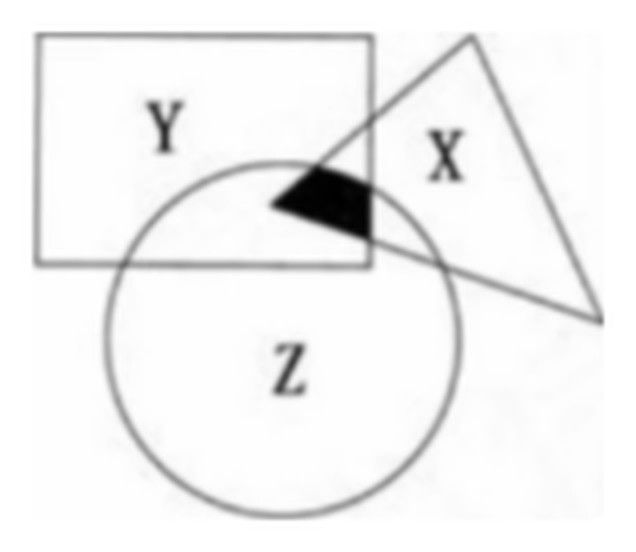
\includegraphics[width=0.20\textwidth]{figures/venn_XYZ_overlap.png}
\end{center}

\ifanswer
\solbegin
\step{设阴影部分的面积是 $x$，则 $290=64+180+160-24-70-36+x$，}
\step{$290=274+x$，$x=16$，故阴影部分的面积是 $16$.}
\solend

\fi

\item 如果集合 $A=\{1,2,3,\cdots,8\}$ 的子集 $B$ 满足：若 $2k\in B$，$k\in\N^{*}$，则 $2k+1\in B$，则称 $B$ 为 $A$ 的“好子集”，$A$ 的“好子集”有 \blankline[2.4em] 个.

\ifanswer
\solbegin
\step{由“好子集”定义得 $2$，$3$ 同时出现，$4$，$5$ 同时出现，$6$，$7$ 同时出现，}
\step{①当集合 $B$ 为空集时，满足题意；}
% 注：原卷此行印作「非空真子集共有 $2^4-1=15$ 种」，与同行算式冲突（$2^4-1=15$ 是**非空子集**数，
%     非空真子集应为 $2^4-2=14$），且与本段①（$B=\varnothing$）合起来恰构成「不含偶数的全体子集」，
%     故按文意订正为「非空子集」（段末总数 $1+15+24+12+2=54$ 不变）。
\step{②当集合 $B$ 中不存在偶数时，$\{1,3,5,7\}$ 的非空子集共有 $2^4-1=15$ 种；}
\step{③当集合 $B$ 中存在 $1$ 个偶数时，三个偶数中选择 $1$ 个，有 $C_3^1=3$ 种，}
\step{剩下 $3$ 个奇数不选，选 $1$ 个、$2$ 个、$3$ 个共有 $2^3=8$ 种，故共有 $24$ 种；}
\step{④当集合 $B$ 中存在 $2$ 个偶数时，三个偶数中选择 $2$ 个，有 $C_3^2=3$ 种，}
\step{剩下 $2$ 个奇数不选，选 $1$ 个、$2$ 个共有 $2^2=4$ 种，故共有 $12$ 种；}
\step{⑤当集合 $B$ 中存在 $3$ 个偶数时，三个偶数中选择 $3$ 个，有 $C_3^3=1$ 种，}
\step{剩下 $1$ 个奇数不选，选 $1$ 个共有 $2^1=2$ 种，故共有 $2$ 种；}
\step{所以 $A$ 的“好子集”共有 $1+15+24+12+2=54$ 种.}
\solend

\fi

\item 已知 $A=\{x\mid x=a^2-b^2,\ a\in\Z,b\in\Z,x\in\N^{*},x\leqslant 40\}$，则集合 $A$ 中共有 \blankline[2.4em] 个元素.

\ifanswer
\solbegin
\step{因为 $(k+1)^2-k^2=2k+1$，所以所有正奇数都属于集合 $A$，}
\step{又 $(2k+2)^2-(2k)^2=8k+4=4(2k+1)$，$(2k+1)^2-(2k-1)^2=8k=4\times 2k$，}
\step{因此所有 $4$ 的整数倍的正整数也属于 $A$，}
\step{若 $x=4k+2$，$k\in\N$，则 $a^2-b^2=(a+b)(a-b)=4k+2=2(2k+1)$，}
\step{则 $a+b$ 和 $a-b$ 中一定是一个取奇数，一个取偶数，}
\step{但是 $a,b\in\Z$ 时，$a+b$ 与 $a-b$ 同奇偶，所以此时无解，}
\step{即所有被 $4$ 除余 $2$ 的正整数都不属于 $A$，}
\step{所以每 $4$ 个数中，有 $3$ 个数属于集合 $A$，则集合 $A$ 中共含 $30$ 个元素.}
\solend

\fi

\item 十个元素组成的集合 $M=\{19,93,-1,0,25,-78,-94,1,17,-2\}$，$M$ 的所有非空子集记为 $M_i$（$i=1,2,\cdots,1023$），每一非空子集中所有元素的乘积记为 $m_i$（$i=1,2,\cdots,1023$），则 $m_1+m_2+\cdots+m_{1023}=$ \blankline[3em].

\ifanswer
\solbegin
\step{因为 $M$ 的所有非空子集为 $M_i$（$i=1,2,\cdots,1023$），这 $1023$ 个子集分成以下几种情况：}
\step{①含 $0$ 的子集有 $512$ 个，这些子集均满足 $m_i=0$；}
\step{②不含 $0$，含 $-1$ 且还含有其它元素的子集有 $255$ 个，}
\step{③不含 $0$，不含 $-1$ 但含有其它元素的子集有 $255$ 个，}
\step{④只含 $-1$ 的子集一个 $\{-1\}$，满足 $m_i=-1$；}
\step{其中②③中的集合是一一对应的，且满足 $m_i$ 对应成相反数，}
\step{故 $m_1+m_2+m_3+\cdots+m_{1023}=512\times 0+255\times 0-1=-1$.}
\solend

\fi

\item 已知 $M=\{(x,y)\mid |xy|=a\}$，$N=\{(x,y)\mid |xy|+1=|x|+|y|\}$，若集合 $M\cap N$ 中的点恰是正八边形的 $8$ 个顶点，则 $a=$ \blankline[2.4em].

\begin{center}
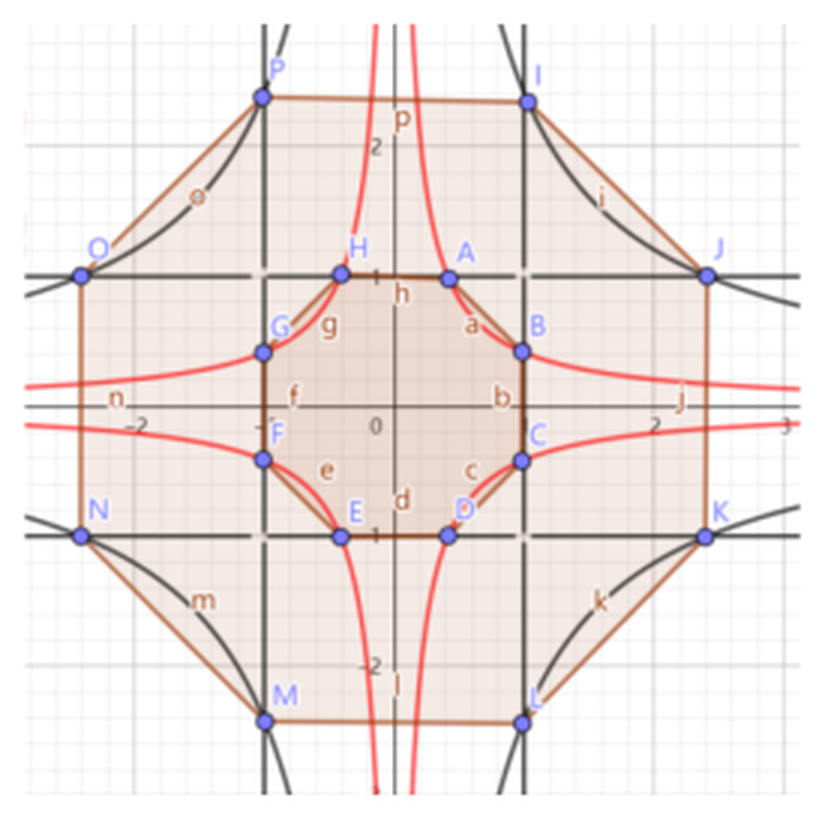
\includegraphics[width=0.44\textwidth]{figures/hyperbola_octagon.png}
\end{center}

\ifanswer
\solbegin
\step{$|xy|=a$ 和 $|xy|+1=|x|+|y|$ 的图像关于坐标轴均对称，只需考虑第一象限即可，}
\step{当 $x>0$，$y>0$ 时，$|xy|+1=|x|+|y|$ 即 $xy+1=x+y$，}
\step{即 $(x-1)(y-1)=0$，}
\step{即 $x=1$ 或 $y=1$，由对称性，作出完整的图像，}
\step{对于 $|xy|=a$，为四段双曲线，}
\step{考虑点 $A(I)(a,1)$，$B(J)(1,a)$，$C(K)(1,-a)$，}
\step{由 $AB=AC$ 得 $\sqrt{(a-1)^2+(1-a)^2}=2a$，解得 $a=\sqrt{2}\pm 1$.}
\solend

\fi

\item 集合 $A$ 是 $\{1,2,3,\cdots,100\}$ 的子集，若 $x\in A$，则 $2x\notin A$，$A$ 中的元素最多有 \blankline[2.4em] 个.

\ifanswer
\solbegin
\step{显然 $51$ 到 $100$ 共 $50$ 个可以，那么从 $1$ 到 $25$ 再 $2$ 倍不会超过 $50$，}
\step{$1$ 到 $25$ 中所有奇数都可以放到子集中，共有 $13$ 个，}
\step{再看偶数，$24=2\times 12$，$22=2\times 11$，$20=2\times 10$，$18=2\times 9$，$16=2\times 8$，}
% 注：末行照原卷抄录。原卷上一行列出 5 个偶数（24、22、20、18、16）而结论写「共有 $50+13+4=67$」，
%     此处的 $4$ 应作「另加 4 个元素」解（穷举验证集合 $A$ 的最大元素数确为 67），非笔误，故不改。
\step{及最后的 $4$，所以，共有 $50+13+4=67$.}
\solend

\fi

\end{enumerate}

\bigsec{二、选择题}

\begin{enumerate}
\setcounter{enumi}{13}

\item 下列各组集合中相等的是（\quad）.

①$P=\{x\mid x=2n,n\in\Z\}$，$Q=\{x\mid x=2(n-1),n\in\Z\}$；

②$P=\{x\mid x^2-1=0\}$，$Q=\left\{x\left|x=\dfrac{1+(-1)^n}{2},n\in\Z\right.\right\}$；

③$P=\{x\mid x=2m+1,m\in\Z\}$，$Q=\{x\mid x=4m\pm 1,m\in\Z\}$；

④$P=\{y\mid y=x^2+1\}$，$Q=\{x\mid y=x^2+1\}$.

\keepwithprev
A. ①②③④\qquad B. ①③\qquad C. ①②④\qquad D. ②④

\ans{B}

\item 如果一个命题的逆命题是真命题，那么这个命题的否命题是（\quad）

\keepwithprev
A. 真命题\qquad B. 假命题

C. 不一定是真命题\qquad D. 不一定是假命题

\ans{A}

\ifanswer
\solbegin
\step{一个命题的逆命题与这个命题的否命题是逆否命题，}
\step{它们的真假性相同，所以逆命题是真命题时，它们的否命题也是真命题. 故选 A.}
\solend

\fi

\item 设 $U$ 表示全集，下列命题中假命题有（\quad）

①若 $A\cap B=U$，则 $A=B=U$；②若 $A\cup B=\varnothing$，则 $A=B=\varnothing$；

③若 $A\cap B=\varnothing$，则 $\overline{A}\cup\overline{B}=U$；④若 $A\cup B=U$，则 $\overline{A}\cap\overline{B}=\varnothing$；

⑤若 $A\subseteq B$，则 $\overline{A}\supseteq\overline{B}$；⑥$\varnothing\in\{\varnothing\}$；⑦$\varnothing\subseteq\{\varnothing\}$.

\keepwithprev
A. $0$\qquad B. $1$\qquad C. $2$\qquad D. $3$

\ans{A}

\ifanswer
\solbegin
\step{全部正确，故选 A.}
\solend

\fi

\end{enumerate}

\bigsec{三、解答题}

\begin{enumerate}
\setcounter{enumi}{16}

\item 已知集合 $A=\{x\mid x^2-3x+2=0\}$，$B=\{x\mid x^2-bx+b-1=0\}$，$C=\{x\mid x^2-cx+2=0\}$.

\begin{enumerate}[label=(\arabic*)]
\item 若 $A\cup B=A$，求实数 $b$ 的值；
\item 若 $A\cap C=C$，求实数 $c$ 的取值范围.
\end{enumerate}

\ifanswer
\solbegin
\stepm{(1)}{$A=\{1,2\}$，$B=\{x\mid(x-1)(x-b+1)=0\}$，}
\step{由 $A\cup B=A$ 得 $b-1=1$ 或 $b-1=2$，所以 $b=2$ 或 $b=3$.}
\stepm{(2)}{由 $A\cap C=C$ 得 $C\subseteq A$，则 $C=\varnothing$ 或 $C=\{1\}$ 或 $C=\{2\}$ 或 $C=\{1,2\}$，}
\step{若 $C=\varnothing$，则 $\Delta=c^2-8<0$，解得 $-2\sqrt{2}<c<2\sqrt{2}$；}
\step{若 $C=\{1\}$，则 $\begin{cases}1+1=c\\ 1\times 1=2\end{cases}$，不可能；}
\step{若 $C=\{2\}$，则 $\begin{cases}2+2=c\\ 2\times 2=2\end{cases}$，不可能；}
\step{若 $C=\{1,2\}$，则 $\begin{cases}1+2=c\\ 1\times 2=2\end{cases}$，符合题意，$c=3$.}
\step{综上所述，$-2\sqrt{2}<c<2\sqrt{2}$ 或 $c=3$.}
\solend

\fi

\ansspace[6]

\item 已知全集 $U=\R$，$A=\{x\mid x^2+px+12=0\}$，$B=\{x\mid x^2-5x+q=0\}$，$\overline{A}\cap B=\{2\}$，求 $p+q$ 的值.

\ifanswer
\solbegin
\step{因为 $\overline{A}\cap B=\{2\}$，所以 $2\in B$，$2\notin A$，}
\step{所以 $2^2-5\times 2+q=0$，解得 $q=6$，$B=\{2,3\}$，}
\step{因为 $\overline{A}\cap B=\{2\}$，$B=\{2,3\}$，所以 $3\in A$，}
\step{所以 $3^2+p\times 3+12=0$，所以 $p=-7$，所以 $p+q=-1$.}
\solend

\fi

\ansspace[5]

\item 求证：方程 $x^2-abx+a+b=0$，$x^2-(a+b)x+ab=0$，其中 $a>2$，$b>2$ 没有公共根.

\ifanswer
\solbegin
\step{假设这两个方程有公共根 $\alpha$，则 $\alpha^2-ab\alpha+(a+b)=0$，$\alpha^2-(a+b)\alpha+ab=0$，}
\step{两式相减得 $(ab-a-b)(\alpha+1)=0$，}
\step{因为 $a>2$，$b>2$，所以 $a-1>1$，$b-1>1$，所以 $(a-1)(b-1)>1$，}
\step{所以 $ab-a-b>0$，所以 $\alpha+1=0$，所以 $\alpha=-1$，}
\step{代入第一个方程，得 $1+ab+a+b=0$，即 $(a+1)(b+1)=0$，}
\step{因为 $a>2$，$b>2$，所以该式不成立，所以这两个方程没有公共根.}
\solend

\fi

\ansspace[9]

% 压轴题：其后已无内容，故作答区全用可丢弃胶水（\ansspace*），并在题目前先量一下版面。
\ansneed{7cm}

\item 若集合 $A$ 具有以下性质：①$0\in A$，$1\in A$；②若 $x$、$y\in A$，则 $x-y\in A$，且 $x\neq 0$ 时，$\dfrac{1}{x}\in A$；则称集合 $A$ 是“好集”.

\begin{enumerate}[label=(\arabic*)]
\item 分别判断集合 $B=\{-1,0,1\}$，有理数集 $\Q$ 是否是“好集”，并说明理由；
\item 设集合 $A$ 是“好集”，求证：若 $x$、$y\in A$，则 $x+y\in A$；
\item 对任意的一个“好集” $A$，分别判断下面命题的真假，并说明理由.

命题 $p$：若 $x$、$y\in A$，则必有 $xy\in A$；

命题 $q$：若 $x$、$y\in A$，且 $x\neq 0$，则必有 $\dfrac{y}{x}\in A$.
\end{enumerate}

\ifanswer
\solbegin
\stepm{(1)}{集合 $B$ 不是“好集”. 理由是：假设集合 $B$ 是“好集”.}
\step{因为 $-1\in B$，$1\in B$，所以 $-1-1=-2\in B$. 这与 $-2\notin B$ 矛盾.}
\step{有理数集 $\Q$ 是“好集”. 因为 $0\in\Q$，$1\in\Q$，}
\step{对任意的 $x$、$y\in\Q$，有 $x-y\in\Q$，且 $x\neq 0$ 时，$\dfrac{1}{x}\in\Q$，}
\step{所以有理数集 $\Q$ 是“好集”.}
\stepm{(2)}{因为集合 $A$ 是“好集”，所以 $0\in A$.}
\step{若 $x$、$y\in A$，则 $0-y\in A$，即 $-y\in A$，所以 $x-(-y)\in A$，即 $x+y\in A$.}
\stepm{(3)}{命题 $p$、$q$ 均为真命题. 理由如下：}
\step{对任意一个“好集” $A$，任取 $x$、$y\in A$，}
\step{若 $x$、$y$ 中有 $0$ 或 $1$ 时，显然 $xy\in A$.}
\step{下设 $x$、$y$ 均不为 $0$，$1$. 由定义得 $x-1$，$\dfrac{1}{x-1}$，$\dfrac{1}{x}\in A$，}
\step{所以 $\dfrac{1}{x-1}-\dfrac{1}{x}\in A$，即 $\dfrac{1}{x(x-1)}\in A$，所以 $x(x-1)\in A$.}
\step{由（2）得 $x(x-1)+x\in A$，即 $x^2\in A$. 同理可得 $y^2\in A$.}
\step{若 $x+y=0$ 或 $x+y=1$，则 $x^2+y^2\in A$.}
\step{若 $x+y\neq 0$ 且 $x+y\neq 1$，则 $(x+y)^2\in A$，}
\step{所以 $2xy=(x+y)^2-x^2-y^2\in A$，所以 $\dfrac{1}{2xy}\in A$，}
\step{由（2）得 $\dfrac{1}{xy}=\dfrac{1}{2xy}+\dfrac{1}{2xy}\in A$，所以 $xy\in A$.}
\step{综上，$xy\in A$，即命题 $p$ 为真命题.}
\step{若 $x$、$y\in A$，且 $x\neq 0$，则 $\dfrac{1}{x}\in A$，}
\step{所以 $\dfrac{y}{x}=y\cdot\dfrac{1}{x}\in A$，即命题 $q$ 为真命题.}
\solend

\fi

\ansspace*[11]

\end{enumerate}

\end{document}
